
\documentclass[ % the name of the author
                    author={Nattanan Nawakitbamrung},
                % the name of the supervisor
                supervisor={Dr. Sébastien Rochat},
                % the degree programme
                    degree={MSc},
                % the dissertation    title (which cannot be blank)
                     title={Developing and Evaluating the Impact of a Single Patient Treatment List (PTL) for an NHS Integrated Care System},
                % the dissertation subtitle (which can    be blank)
                  subtitle={},
                % the dissertation     type
                      type={},
                % the year of submission
                      year={2025}]{dissertation}


\usepackage{multirow}
\usepackage{booktabs,tabularx}
\usepackage{adjustbox}
\usepackage{subcaption} 
\usepackage{placeins} 
\usepackage{graphicx}

\begin{document}

% =============================================================================

% This section simply introduces the structural guidelines.  It can clearly
% be deleted (or commented out) if you use the file as a template for your
% own dissertation: everything following it is in the correct order to use 
% as is.

% =============================================================================

% This macro creates the standard UoB title page by using information drawn
% from the document class (meaning it is vital you select the correct degree 
% title and so on).


\maketitle

% After the title page (which is a special case in that it is not numbered)
% comes the front matter or preliminaries; this macro signals the start of
% such content, meaning the pages are numbered with Roman numerals.

\frontmatter

% This macro creates the standard UoB declaration; on the printed hard-copy,
% this must be physically signed by the author in the space indicated.

\makedecl

% LaTeX automatically generates a table of contents, plus associated lists 
% of figures, tables and algorithms.  The former is a compulsory part of the
% dissertation, but if you do not require the latter they can be suppressed
% by simply commenting out the associated macro.

\tableofcontents
\listoffigures
\listoftables
\listofalgorithms
% \lstlistoflistings 

% The following sections are part of the front matter, but are not generated
% automatically by LaTeX; the use of \chapter* means they are not numbered.

% -----------------------------------------------------------------------------

\chapter*{Abstract}
\noindent
This dissertation addresses the operational challenge of the NHS Cambridgeshire and Peterborough Integrated Care System (ICS), where fragmented Patient Treatment Lists (PTLs) across multiple providers create systemic inefficiencies in resource allocation, inequities in access, and prolonged patient waiting times. Using the cataract treatment pathway as a case study, the research tackles the complex problem of uncoordinated scheduling and capacity management in a multi-provider environment.

\vspace{0.2cm}
A high-fidelity, data-driven discrete-event simulation framework was developed to model patient flows under realistic constraints, including variable case complexity levels (low, medium, high), general anaesthetic (GA) requirements, provider-specific service times, capacity in daily operative minutes, and selective case acceptance by independent providers. Empirical NHS data for 2023/24, augmented with synthetic generation preserving real-world distributions, was used to replicate baseline operations for comparison.

\vspace{0.5cm}
\noindent
Multiple allocation strategies were systematically evaluated, spanning:
\begin{quote}
    \begin{itemize}
        \item Shared PTL approaches (equal distribution, capacity-weighted, shortest-wait greedy)
        \item Equity-focused approaches (complexity-balanced allocation) to mitigate provider complexity skew
        \item Financially oriented approaches (fee-biased)
        \item NHS-first fallback strategies for GA and high-complexity cases
        \item An experimental machine learning policy predicting provider-specific wait times and selecting top candidates with fallback simulation
    \end{itemize}
\end{quote}

Key performance metrics included mean waiting time, proportion treated within policy targets, provider utilization, travel distance, equity in complexity distribution, and tariff-based revenue.

\noindent
Key results show that:
\begin{quote}
    \begin{itemize}
        \item Baseline policy reproduced real-world disparities (mean wait 112.1 days, 10.54\% treated within 30 days.
        \item Complexity-Balanced allocation preserved a 50/50 complexity split between NHS and independent providers, with mean wait 85.62 days and 52.05\% \% treated within 90 days..
        \item Fee Biased reduced waits to 96.81 days but left 6.37\% unassigned and caused severe inequity in case mix.
        \item The ML Top-3+Fallback policy demonstrated the feasibility of integrating predictive modeling into PTL allocation, though current implementation did not outperform rule-based best policies due to capacity bottlenecks, single-day prediction horizons, and lack of global rebalancing.
    \end{itemize}
\end{quote}

\vspace{3cm}
\noindent
A summary of main contributions:
\begin{quote}
    \begin{itemize}
        \item Development of a robust simulation platform integrating real-world data, realistic operational constraints, and provider behavior.
        \item Comparative evaluation of 18 allocation strategies, including both rule-based and machine learning–assisted approaches, under operational constraints such as GA requirements and case complexity.
        \item Quantitative demonstration that coordinated, capacity- and complexity-aware PTL management can reduce mean waits by over 90% while improving equity and maintaining high utilisation.
        \item Introduction of a transferable framework for simulating, testing, and comparing healthcare allocation policies, applicable to other specialties and ICS contexts.
        \item Provision of actionable evidence to support ICS-level decision-making, alongside identification of future improvements in predictive capacity-aware scheduling, multi-day lookahead, and global optimization.
    \end{itemize}
\end{quote}

% -----------------------------------------------------------------------------

% \chapter*{Summary of Changes}

% {\bf A conditional section, of at most $1$ page} 
% \vspace{1cm} 

% If (and only if) the dissertation represents a resubmission (e.g., as the result of
% a resit), then this section is compulsory: the content should summarise all
% non-trivial changes made to the initial submission.  Otherwise you can
% omit it, since {\bf a summary of this type is only needed for resubmissions}.

% When included, the section will ideally be used to highlight additional
% work completed, and address criticism raised in any associated feedback.
% Clearly it is difficult to give generic advice about how to do so, but
% an example might be as follows:

% \begin{quote}
% \noindent
% \begin{itemize}
% \item Feedback from the initial submission criticised the design and 
%       implementation of my genetic algorithm, stating ``there seems 
%       to have been no attention to computational complexity during the
%       design, and obvious methods of optimisation are missing within
%       the resulting implementation''.  Chapter 3 now includes a
%       comprehensive analysis of the algorithm, in terms of both time
%       and space.  While I have not altered the algorithm itself, I
%       have included a cache mechanism (also detailed in Chapter 3)
%       that provides a significant improvement in average run-time.
% \item I added a feature in my implementation to allow automatic rather
%       than manual selection of various parameters; the experimental
%       results in Chapter 4 have been updated to reflect this.
% \item Questions after the presentation highlighted a range of related
%       work that I had not considered: I have make a number of updates 
%       to Chapter 2, resolving this issue.
% \end{itemize}
% \end{quote}

% -----------------------------------------------------------------------------

\chapter*{Supporting Technologies}
\begin{quote}
\noindent
\vspace{-0.5cm}
\begin{itemize}
    \item \textbf{Programming language and environment:}
    \begin{itemize}
        \item Python was the primary language used for all simulation modeling, data processing, and analysis.
        \item Jupyter Notebook was used for exploratory data analysis.
        \item The simulation framework and policy functions were implemented as standalone Python modules.
    \end{itemize}

    \item \textbf{Python packages and libraries:}
    \begin{itemize}
        \item \texttt{pandas} for data manipulation and CSV file I/O.
        \item \texttt{numpy} for numerical computations.
        \item \texttt{matplotlib} for generating visualizations and plots.
        \item \texttt{tqdm} for progress tracking in simulation loops.
        \item \texttt{random} and \texttt{datetime} for patient arrival generation, scheduling, and date manipulations.
        \item \texttt{collections} (\texttt{defaultdict}) for patient grouping and allocation logic.
    \end{itemize}

    \item \textbf{Machine learning tools:}
    \begin{itemize}
        \item \texttt{scikit-learn} for training classification and regression models for provider assignment prediction and wait time estimation.
    \end{itemize}

    \item \textbf{Geospatial computation:}
    \begin{itemize}
        \item Haversine formula implementation for calculating travel distances between patient and provider coordinates.
    \end{itemize}

    \item \textbf{Datasets:}
    \begin{itemize}
        \item Patient-level data with arrival dates, HRG codes, complexity, GA flag, coordinates, and tariffs.
        \item Provider name, NHS/independent status, latitude, longitude.
        \item Historical throughput per provider and complexity.
        \item Mapping from LSOA codes to latitude/longitude for patient location generation.
        \item Synthetic datasets generated for counterfactual policy simulations and stress testing.
    \end{itemize}

    \item \textbf{Document preparation:}
    \begin{itemize}
        \item The dissertation was written in \LaTeX{} and formatted using the online service \emph{Overleaf}.
    \end{itemize}
\end{itemize}

\end{quote}

% -----------------------------------------------------------------------------

% \chapter*{Notation and Acronyms}

% {\bf An optional section, of roughly $1$ or $2$ pages}
% \vspace{1cm} 

% \noindent
% Any well written document will introduce notation and acronyms before
% their use, {\em even if} they are standard in some way: this ensures 
% any reader can understand the resulting self-contained content.  

% Said introduction can exist within the dissertation itself, wherever 
% that is appropriate.  For an acronym, this is typically achieved at 
% the first point of use via ``Advanced Encryption Standard (AES)'' or 
% similar, noting the capitalisation of relevant letters.  However, it 
% can be useful to include an additional, dedicated list at the start 
% of the dissertation; the advantage of doing so is that you cannot 
% mistakenly use an acronym before defining it.  A limited example is 
% as follows:

% \begin{quote}
% \noindent
% \begin{tabular}{lcl}
% AES                 &:     & Advanced Encryption Standard                                         \\
% DES                 &:     & Data Encryption Standard                                             \\
%                     &\vdots&                                                                      \\
% ${\mathcal H}( x )$ &:     & the Hamming weight of $x$                                            \\
% ${\mathbb  F}_q$    &:     & a finite field with $q$ elements                                     \\
% $x_i$               &:     & the $i$-th bit of some binary sequence $x$, st. $x_i \in \{ 0, 1 \}$ \\
% \end{tabular}
% \end{quote}

% -----------------------------------------------------------------------------

\chapter*{Acknowledgements}

\noindent
I am deeply grateful to \textbf{Dr.~Sébastien Rochat} for his academic guidance, careful advice, and generous time throughout this project.

I would also like to thank \textbf{Joao Rocha}, \textbf{Joe Esgate}, and \textbf{Sue Somers} (NHS Cambridgeshire and Peterborough ICB) for their thoughtful suggestions and detailed feedback that substantially improved the quality of this work.

My thanks extend to the \textbf{Cambridgeshire and Peterborough ICS} for providing contextual guidance on service delivery and access to data. All datasets were anonymised and processed in line with the data-sharing agreement and research ethics requirements.

Finally, I thank my family and friends for their encouragement and patience during the thesis writing process. Any remaining errors or omissions are entirely my own.


% =============================================================================

% After the front matter comes a number of chapters; under each chapter,
% sections, subsections and even subsubsections are permissible.  The
% pages in this part are numbered with Arabic numerals.  Note that:
%
% - A reference point can be marked using \label{XXX}, and then later
%   referred to via \ref{XXX}; for example Chapter\ref{chap:context}.
% - The chapters are presented here in one file; this can become hard
%   to manage.  An alternative is to save the content in seprate files
%   the use \input{XXX} to import it, which acts like the #include
%   directive in C.

\mainmatter

% -----------------------------------------------------------------------------

% {\bf A compulsory chapter, roughly 10\% of the total page-count}
% \vspace{1cm} 

% putting a \noindent before the first para in each chapter looks nicer.
% This chapter should describe the project context, and motivate each of
% the proposed aims and objectives.  Ideally, it is written at a fairly 
% high-level, and easily understood by a reader who is technically 
% competent but not an expert in the topic itself.

% In short, the goal is to answer three questions for the reader.  First, 
% what is the project topic, or problem being investigated?  Second, why 
% is the topic important, or rather why should the reader care about it?  
% For example, why there is a need for this project, who will benefit from the 
% project and in what way (e.g., clients/end-users who needed some analysis
% done, or other data scientists who might need the tools you have developed), what 
% work does the project build on and why is the selected approach either
% important and/or interesting (e.g., fills a gap in literature, applies
% results from another field to a new problem).  Finally, what are the 
% central challenges involved and why are they significant? 
 
% The chapter should conclude with a concise bullet point list that 
% summarises the aims, objectives, {\bf and achievements}\/ of your work. 
\chapter{Introduction}
\label{chap:introduction}

\noindent
\section{Background and Problem Statement}
A major and current challenge for the United Kingdom's National Health Service (NHS) is the management of extensive waiting list for planned medical treatments. \cite{nuffield2024dashboard, kingsfund2024}. This issue impacts patients’ quality of life, leads to poorer clinical outcomes, and strains on healthcare resources. These problems are often made worse by underlying structural inefficiencies in the system's design \cite{nhs2024guide, nuffield2024hospital}.

\vspace{0.2cm}
This dissertation, conducted in collaboration with the Cambridgeshire and Peterborough Integrated Care System (ICB), investigates these challenges within the specific context of the cataract surgery pathway. The ICB currently operates with multiple, separate Patient Treatment Lists (PTLs), where each healthcare provider both NHS and Independent Sector (IS) manages its own queue. This disconnected structure disrupt the effective sharing of workload and resources, preventing a provider with available capacity from easily treating patients on another's long list. This systemic structure block effective workload balancing and prevents providers with spare capacity from easily treating patients on another provider’s longer list \cite{healthwatch2025strain, ihpn2025stats}.

\vspace{0.2cm}
Initial analysis of the ICB's data shows a imbalance in case mix and throughput between sectors: independent providers treat a higher proportion of low-complexity cataract cases, while NHS providers treat the majority of high-complexity and general anesthetic (GA) cases \cite{nhs2022elective, rcophth2021audit}. This pattern may come from systemic incentives, referral behavior, and training requirements \cite{elalouf2013fair, rawls1971theory}, and results in under-utilization of potential system-wide capacity.

\vspace{0.2cm}
This observed imbalance leads to the central strategic question posed by the ICB, which forms the core of this research: If triage were centralized, what would be the optimal strategy for allocating patients across this heterogeneous network of providers? To answer this, this project develop a Discrete-Event Simulation (DES) platform to model and compare various allocation strategies, enabling systematic testing of multiple rule-based and machine learning–assisted allocation strategies under realistic policy solutions. 

\section{Aim and Objectives}
The primary aim is to develop and evaluate centralized allocation strategies for the cataract surgery pathway that improve efficiency, equity, and utilization across the ICB network.

\vspace{0.5cm}
\noindent
This involves two key missions:
\begin{enumerate}
    \item To analyze system imbalance by simulating current operations and identifying its drivers.
    \item To design and test optimal allocation policies that balance the competing objectives of:
    \begin{itemize}
        \item Efficiency: Minimizing overall patient waiting times.
        \item Equity: Distributing case complexity more evenly to reduce bottlenecks.
        \item Patient Experience: Maintaining reasonable travel distances.
    \end{itemize}
\end{enumerate}

\vspace{1cm}
\noindent
Specific objectives are to:
\begin{itemize}
    \item Develop a DES model reflecting real-world operation, case complexity, and GA requirements \cite{simpy_docs}.
    \item Analyze current system dynamics to identify causes of imbalance in throughput and complexity distribution.
    \item Design and evaluate a range of centralized allocation policies, including rule-based and machine learning–assisted approaches \cite{scikit_learn_api}.
    \item Quantitatively assess each policy using efficiency, equity, and utilization metrics.
    \item Provide evidence-based policy recommendations to the ICB, highlighting trade-offs and implementation considerations.
\end{itemize}

\noindent
\section{Research Questions}

To address the strategic challenge posed by the ICB, this project seeks to answer one primary research question, supported by four secondary questions that guide the investigation into the system's complex dynamics.

\noindent
\subsection{Primary Research Question}

What is the optimal central allocation strategy for the cataract surgery pathway that balances minimizing waiting times, accommodating provider heterogeneity (case mix, performance, training), and maintaining system equity?
\noindent
\subsection{Secondary Research Questions}
\begin{itemize}
    \item What systemic factors (e.g., incentives, referral patterns) drive the current imbalance between NHS and independent providers?
    \item How much can dynamic, efficiency-focused allocation policies reduce waiting times, and what trade-offs arise in patient travel and equity?
    \item How do complexity-balancing strategies affect equity and NHS training requirements?
    \item What is the probability and performance impact of incorporating machine learning–based predictions into PTL allocation?
\end{itemize}

\noindent
\section{Scope and Delimitation}

\noindent
\subsection{Scope of the Research}
\begin{itemize}
    \item \textbf{Primary focus:} Development, simulation, and evaluation of a single, centralized PTL model with multiple allocation strategies.
    \item \textbf{Clinical pathway:} Cataract surgery in Cambridgeshire & Peterborough ICB.
    \item \textbf{Methodology:} Discrete-Event Simulation, with rule-based and ML-assisted policy design.
    \item \textbf{Data:} Empirical NHS data supplemented with synthetic data for scenario and stress testing.
    \item \textbf{KPIs:} Mean/max wait time, throughput, utilization, equity in case mix, tariff, and travel distance \cite{pandas_docs}.
\end{itemize}

\noindent
\subsection{Delimitation}
\begin{itemize}
    \item This study is based on the use of historical and monthly data. The model is designed as a strategic planning and evaluation tool and does not operate on or require real-time data feeds.
    \item The model focuses on elective cataract surgery and does not include emergency care pathways.
    \item ML experiments focus on probability and proof-of-concept rather than full operational deployment.
\end{itemize}

% -----------------------------------------------------------------------------

\chapter{Background}
\label{chap:background}

\vspace{1cm} 

\noindent
This chapter provides both the contextual and the technical foundations for the research. 
It begins by outlining the current operational challenges in the NHS cataract surgery pathway, highlighting why the allocation of patients across providers is a critical issue. It then introduces the conceptual of allocation strategies and explains the rationale for using Discrete-Event Simulation (DES) as the primary methodological tool. This combination of contextual and methodological framing ensures that the reader understands not only \emph{what} problem is being addressed, but also \emph{how} and \emph{why}.

\section{Contextual Background}

Before discussing the methodological approach, it is essential to understand the current pressures and structural issues within NHS England’s elective care system. This context clarifies why cataract surgery, in particular, is used as the focal point for modeling allocation strategies.

\subsection{The NHS Elective Care Crisis}
The currently NHS England systemic is facing the largest elective waiting list crisis ever in history. As of May 2025, data show that there were 7.36 million patients waiting to start treatment in NHS hospitals, with only around 60\% receiving treatment within 18 weeks being referred. This is below the NHS England target of 92\%, which is a goal that has not been met since 2015 \cite{nhs2024guide, nuffield2024dashboard, kingsfund2024}.

\vspace{0.2cm}
In ophthalmology, which is one of the highest surgical volumes of in the NHS data from December 2024 indicate that approximately 59,000 patients were on the waiting list for specialist eye care, and only 66.8\% were treated within 18 weeks \cite{healthwatch2025strain}. In some hospital such as Chesterfield Royal Hospital and Dorset County Hospital, patient may wait 39-45 weeks for cataract surgery \cite{practiceplus2025waiting}.

\vspace{0.2cm}
Following the COVID-19 pandemic, the Independent Sector (ISPs) contracted with the NHS has significantly reduced waiting lists. Recent figures show that IS patients wait on average 11.5 weeks compare with 18 weeks in the NHS, and only 1.1\% of IS patient wait over one year compared with 3\% in the NHS \cite{ihpn2025stats}. This difference highlights both the potential and the limitation caused by discontinuities between sectors in the healthcare system.

\subsection{The Mixed-Economy Model and Commissioning}
NHS England operate in a mixed-economy model, meaning that care is provided both by public NHS Trusts and by private sector services contracted with the NHS known as Independent Sector Providers (ISPs). ISPs play a significant and growing role in delivering elective care, especially cataract surgery, which is high-volume and low-risk. Their contribution has increased since the COVID-19 crisis, helping to reduce elective backlogs \cite{ihpn2025stats, kingsfund2023backlog}.

\vspace{0.2cm}
Commissioning is the responsibility of Integrated Care Boards (ICBs), which assess the population needs, plan services, and contract with provider. Contracts typically specify  workload volumes, payment according to the national tariff, and quality standard \cite{nhs2022elective}. In ophthalmology, ICBs procure service from both the NHS and ISPs, which often maintain separate Patient Treatment Lists (PTLs) and independent referral routes \cite{kingsfund2023backlog}.

\vspace{0.2cm}
Although this structure expands the overall system's capacity, in practice it creates operational "silos" between providers. Patients are often referred only to contracted providers, preventing the use of spare capacity in one provider queues in another \cite{ifs2024past}.This situation contributes to imbalances in case mix and workload between the sectors: the NHS receives a higher proportion of high-complexity cases requiring general anaesthesia (GA), while ISPs tend to receive primarily low-complexity cases \cite{healthwatch2025strain, rcophth2021audit}. This inequity is a key motivation of developing a centralized triage and allocation system, which forms the core of this research.

\subsection{Why Ophthalmology (Especially Cataract) is Crucial}
Cataract surgery is the highest-volume planned procedure in NHS England, accounting for more than 10\% of all planned operations and exceeding 500,000 procedures per year \cite{rcophth2021audit}. Key factors contributing to cataract's significance include:
\begin{enumerate}
    \item \textbf{Population aging} - The arise  number of cataract is directly proportional to the increase in age, driving growing demand for surgery \cite{who2023cataract}.
    \item \textbf{Impact on quality} of life - Blindness and vision impairment directly affects daily functioning and increased risk of falls in the elderly.
    \item \textbf{Equity concerns} – The NHS often handles higher proportions of complex and GA-requiring cases, leading to disparities in workload.
\end{enumerate}
\subsection{The Cataract Surgery Pathway}
The cataract pathway in the NHS consists of six main steps \cite{girft2022cataract}:
\begin{enumerate}
    \item Referral - From an optometrist or general practitioner (GP) after an initial diagnosis.
    \item Triage \& PTL Registration - Assessing complexity (Low/Medium/High), need for GA, and priority level (1–3) before PTL entry.
    \item Scheduling \& Allocation - Assessing the patient to a provider and scheduling surgery within capacity limits.
    \item Pre-operative Assessment - Physical examination and preparation before surgery
    \item Surgery - Cataract surgery is performed using local anesthesia (LA) or general anesthesia (GA) as needed.
    \item Post-operative Follow-up - Post-operative follow-up and care.
\end{enumerate}
This research focuses on steps 2 and 3, as these are the decision points where allocation policy directly affects waiting time, equality and resource utilization.
\subsection{Systemic Challenges and Inefficiencies}
From initial analysis and literature review, several structural issues were identified:
\begin{itemize}
    \item \textbf{System Fragmentation} - Multiple separate PTLs make it difficult to allocate capacity across providers.
    \item \textbf{Imbalance of case mix} - NHS providers receive a higher share of high-complexity cases, creating bottlenecks and affecting training capacity.
    \item \textbf{Financial Incentive} - Payment by Results and tariff structure may create selection of low-complexity, short-duration case \cite{elalouf2013fair, rawls1971theory}.
    \item \textbf{Effect} - There issues lead to delays, inequities in access, and under-utilization of resources.
\end{itemize}

\section{Related Work and Existing Approaches}
In addition to understanding the NHS contextual background of cataract surgery, conducting a literature review is an important step to identify gaps in existing knowledge and to provide a foundation for improving patient allocation and simulation approaches that are appropriate to the context of this research.

\subsection{The use of Discrete-Event Simulation (DES) in public health resource allocation}
\paragraph{Demir et al. (2018)} \cite{demir2018des} developed a DES model to simulate the cataract surgery treatment pathway in the NHS using real data from Leicester Royal Infirmary. This model was used to evaluate the impact of new policies on capacity, productivity, and waiting lists. The study found that the number of surgeries could be increased by around 40\% without increasing the budget. However, the model remains limited to a single-provider level and does not consider multi-sector contexts or workload distribution across organizations.

\paragraph{NHS Scotland, Scottish Government (2025)} \cite{scotgov2025des} used DES to analyse "what-if" scenarios by evaluating changes in productivity and patient pathways. For example, booking second-eye surgery immediately after the first-eye operation significantly reduced the waiting list size. This work emphasizes that the level of detail in modeling patient flow has a significant on simulation outcomes.

\paragraph{NIHR ARC SWP (2022)} \cite{nihr2022pifu} used DES to test the Patient Initiated Follow-Up (PIFU) policy in rheumatology within NHS England. The results showed that waiting lists could be reduced approximately 10 weeks. Although not directly related to ophthalmology, but this is an example of applying simulation-based policy modeling to reduce elective care backlogs.

\subsection{Mixed-Economy Public-Private Workload Balance}
\paragraph{Nuffield Trust, King’s Fund and IHPN} \cite{nuffield2024hospital, kingsfund2023backlog, ihpn2025stats} reported and analyzed  policies regarding case-mix imbalance and the effects of workload transfers to the independent sector. However, most of this works focus on descriptive analytics rather than simulation modeling. The literature review indicates that there is limited work on simulations systems that include multi-provider, multi-sector while actively managing workloads between NHS and ISPs in the context of cataract surgery.

\subsection{Operational Research & Optimization in Cataract Surgery}
In practical operations within cataract surgery, some research has used DES alongside capacity planning, such as Demir et al. (2018) \cite{demir2018des}, which combined demand forecasting with simulation. However, these models often not incorporate realistic constraints such as case-mix balance or general anaesthesia (GA) slot limitations.

In term of optimization, there is relatively little work that integrates Machine Learning, Linear Programming or other advanced OR techniques with simulation to perform multi-policy testing under realistic NHS operational constraints.

\subsection{Research Gaps}
From the literature review, the following gaps were identified:
\begin{itemize}
    \item Most of research focuses on single-provider contexts, rather than multi-sector or multi-provider systems.
    \item Few models incorporate realistic constraints such as case-mix, GA slot, and capacity limitations.
    \item Few existing model comprehensively tests multiple policy scenarios within a realistic NHS operational environment.
\end{itemize}
This research focuses on creating a Discrete-Event Simulation to model a multi-provider system. It covers practical constraints and evaluates multiple policy models, with particular on capacity, equity, and general anaesthesia requirements.

\clearpage

\subsection{Adaptation from Previous Works}
To ensure that the design and development of the model in this research are connected to the existing knowledge base, concepts and components from previous studies have been adapted as follows:
\noindent
\begin{table}[h!]
\centering
\renewcommand{\arraystretch}{1.25}    
\setlength{\tabcolsep}{6pt}            
\begin{tabular}{|p{2.5cm}|p{5cm}|p{3.5cm}|p{3.5cm}|}
\hline
\textbf{Literature} & \textbf{Key concept / method used} & \textbf{Application in This Research} & \textbf{Extended} \\
\hline
Demir et al. (2018) &
DES patient flow for cataract surgery (single provider). & 
Using SimPy to simulate patient arrival, queue, and service time.&
Multi‑provider, added GA constraint, complexity constraints and multiple policy. \\
\hline
Scottish Government (2025) &
“What‑if” scenario DES on waiting lists. &
Scenario testing of policy allocation. &
Scenario tests under realistic capacity and complexity constraints. \\
\hline
Nuffield Trust, King’s Fund, IHPN &
Analysis of NHS–ISP case-mix imbalance. &
Used an initial condition for complexity‑balanced design. &
Developed complexity-balanced policy to reduce imbalance. \\
\hline
GIRFT Cataract Pathway &
Standard NHS pathway (referral $\rightarrow$ triage $\rightarrow$ allocation $\rightarrow$ surgery $\rightarrow$ follow‑up). &
Used pathway as a framework in \textbf{simulate()} &
Added Shared‑PTL centralized allocation overlay on pathway \\
\hline
Elalouf (2013), Rawls (1971) &
Fairness principles for equitable allocation. &
Applied in complexity-balanced policy&
Combined equity principles with capacity and operational feasibility in simulation.\\
\hline
\end{tabular}
\caption{Adaptation from previous works}
\label{tab:adaptation}
\end{table}

\section{Technical and Methodology Background}
This section examines the technical and methodological aspects of the research, covering the simulation framework, secenario creation, data preparation, and evaluation metrics. The aim is to ensure that the simulation system and allocation pathway are robust, repeatable, and expandabele for future work.

\subsection{Discrete-Event Simulation: DES}
The simulation was developed using \texttt{SimPy}, a Python library for discrete-event simulation (DES). This approach was chosen because it supports time-ordered simulation, making it well-suited to representing processes such as patient acceptance, queuing, and service processes. It also allows precise control of service time, capacity, and patient attributes, and supports complex operational rules such as the GA requirement or provider restrictions for high-complexity cases. In the model, each patient is represented as an entity with attributes such as complexity, GA requirement, priority, and tariff. Providers are represented as resources with a daily capacity measured in minutes. The simulation clock progresses event by event until all patients are allocated.

\subsection{Development and Work of Allocation Policy}
Allocation policies were developed to compare outcomes in term of waiting, utilization, and equity. Each policy is implemented as a Python function (e.g., \texttt{baseline\_policy()}, \texttt{complexity\_balanced\_policy()}, \texttt{greedy\_policy()}) with the following steps:
\begin{itemize}
    \item Select a provider based on rule-based such as nearest distance, shortest queue, and capacity-weighted distribution. 
    \item Apply acceptance rules via the \texttt{provider\_accepts()} function (e.g., GA cases always go to NHS, high-complexity cases may have provider restrictions).
    \item Dynamically update provider queues in each simulation round.
\end{itemize}

\subsection{Data Preprocessing and Inputs}
The simulation uses both real NHS data (2024/2025) and synthetic data generated from previous years: 
\begin{itemize}
    \item \textbf{Real Data}: NHS cataract surgery data, provider capacity, and pathway information. 
    \item \textbf{Synthetic Data}: Generate using the empirical distribution of real data to maintain realistic characteristics used to expand patient number and trigger bottleneck events.
    \item \textbf{Provider Data}: Includes NHS/ISP status, latitude, longtitude, and daily capacity.
\end{itemize}
Travel distance between patient's LSOA area and provider is calculated using the geodesic method. Surgery duration is determined by case complexity and provider type.

\subsection{Application of previous work to the methodology}
Several concepts from previous research (Table~\ref{tab:adaptation}) were adapted. The DES patient-flow structure from Demir et al. (2018) was extended to a multi-provider setting. The scenario-testing approach from Scottish Government (2025) was incorporated to evaluate policy alternatives. Complexity-balanced allocation was inspired by recommendations from the Nuffield Trust and King’s Fund. The simulation pathway structure follows the GIRFT Cataract Pathway, forming the core patient journey in the model.

\subsection{Evaluation indicators}
Key metrics for assessing policy performance include: 
\begin{itemize}
    \item Average and maximum waiting time (days).
    \item Standard deviation of waiting times.
    \item Percentage of patients treated within 7, 30, and 90 days.
    \item Average travel distance (km).
    \item Daily utilization rate (\% of capacity used).
    \item Total tariff value.
    \item Case-mix distribution between NHS and ISP for each complexity level.
\end{itemize}

\subsection{Software and Repeating result}
The simulation was implemented in Python 3.12, using \texttt{SimPy} for DES, \texttt{Pandas} and \texttt{NumPy} for data processing, \texttt{Geopy} for travel distance calculation, and \texttt{Matplotlib} for visualization. All scripts are modular and parameterized, allowing experiments to be easily replicated extended for new policy scenarios.

\subsection{Simulation Workflow}
To clarify how the simulation operates, a workflow diagram is presented in Figure~\ref{fig:sim-workflow}. The workflow starts with data inputs (both real NHS data and synthetic data) and continues through policy selection, eligibility checks, allocation and scheduling of patients, and discrete-event execution. 
The final stage is the output log, which records events and produces evaluation metrics. This workflow presents the full pipeline of the simulation process and provides a visual reference for how patients are allocated and processed under different policy scenarios.

\begin{figure}[t]
\centering
\includegraphics[width=0.9\linewidth]{fig/simulation_workflow.png}
\caption{Simulation workflow.}
\label{fig:sim-workflow}
\end{figure}
% -----------------------------------------------------------------------------

\chapter{Execution}
\label{chap:execution}

\section{Design Decisions}
In developing the Discrete-Event Simulation (DES) for patient allocation in the Cambridgeshire and Peterborough Integrated Care System's Patient Treatment List (PTL), several design decisions were made to ensure the model reflects the real-world practice as closely as possible, while still maintaining flexibility to test wide range of policies. These decisions are summarised in the following subsections.

\subsection{Simulation Time-step and Capacity Modeling}
The simulation was designed to operate in daily steps rather than weekly or monthly intervals. This choice reflects the fact that, in practice cataract surgery schedules are organized on a daily basis. A daily step allows the model to capture fluctuations in provider capacity and patient arrivals more accurately, and it also aligns with structure of the real dataset, which records admission at the daily level.

\vspace{0.2cm}
Regarding capacity, instead of defining it as a fixed number of slot per day, the model represents provider availability as a total number of minutes per day. This daily capacity is then divided by the service time required for each patient. Service time varies according to both the complexity of the case (low, medium, high) and the type of provider (NHS or independent). This approach provides a more realistic reflection of performance differences and the impact of complex cases than a simple slot-based allocation.

\subsection{Acceptance Rules}
Two main rules were introduced to reflect clinical constraints:
\begin{itemize}
    \item \textbf{General Anaesthesia (GA)} patient can only be treated by NHS providers, because most independent providers are not equipped with anesthesia services.
    \item \textbf{High complexity} patients are typically directed to the NHS. However, this restriction can be toggled on or off (via the \texttt{provider\_accepts()} function) to support counterfactual policy testing in which the private sector may also admit complex patients.
\end{itemize}

\subsection{Logging and Metrics}
Simulation outputs are recorded at two levels:
\begin{itemize}
    \item \textbf{Patient-level}, including waiting time, assigned provider, travel distance and tariff.
    \item \textbf{Provider-level}, including resource utilization, actual patient volume, and financial returns.
\end{itemize}
Separating the data in this way allows for both micro-level analysis of patient experience and macro-level evaluation of system performance.

\vspace{0.2cm}
\noindent
To evaluate each policy, multiple metric are considered. These include the average and standard deviation of waiting time, the percentage of patient 
treated within 7, 30, and 90 days, average travel distance, provider utilization, and tariff. The use of multidimensional indicators allows for a more comprehensive comparison between polices, balancing efficiency and equity.

\subsection{Policy Architecture}
The model was designed to support a wide range of policies by separating policy logic from simulation engine. All policy functions are defined within a \texttt{policy.py} module, independent of the core simulation engine. This modular structure makes it easier to add or remove policies without impact the simulation backbone. Policies implemented include the baseline policy, complexity-balanced policy, fee-biased policy, and machine learning-based balanced policy.

\vspace{0.2cm}
Each simulation run is configured with a fixed random seed to control randomness. Configuration parameters are stored separately from the main code to ensuring that experiments can be reproduce and independently verified.

\vspace{0.5cm}
\noindent
In summary, these design decisions ensure that the simulation achieves both realism and flexibility, two essential conditions for experimenting with counterfactual policies under a centralized PTL system.

\section{Simulation Architecture and Implement}
The simulation architecture is designed to be a modular by separating the system into three layers.
\begin{enumerate}
    \item \textbf{Core Simulation} performs daily-step simulation, control the timeline, provider capacity (minuted per day), and status updates. 
    \item \textbf{Policy Layer} is a module that receives the active patient and returns a ranked list of suitable providers for each day according to the specified criteria and clinical rules.
    \item \textbf{I/O and Logging Layer} records patient and provider-level outputs for subsequent evaluation.
\end{enumerate}
As illustrated in Figure ~\ref{fig:comp-arch}, policies interact with the core engine via a standard interface, while logging components collect patient and provider-level events for metric computation.

\begin{figure}[htbp]
\centering
\includegraphics[width=0.9\linewidth]{fig/component_diagram.png}
\caption{Component diagram of the simulation system}
\label{fig:comp-arch}
\end{figure}

\subsection{Key components of the model}
The key components consist of two entity: \texttt{Patient} and \texttt{Provider}. The \texttt{Patient} entity stores decision-relevant attributes such as complexity, need for GA, priority level, HRG code, and geographic location (lat/lon). In contrast, the \texttt{Provider} entity stores provider information such as sector type (NHS or Independent), total service time available per day (minutes per day), and methods to eligibility checking (\texttt{can\_accept()}) and allocation (\texttt{assign\_patient()}).

A key function for determining service time per patient is \texttt{get\_service\_time(patient, provider)}, which depends on patient complexity and provider type. In addition, the \texttt{provider\_accepts()} function enforces clinic constrain for example, GA cases are treated by NHS only, and high-complexity cases may restricted to the NHS depends on policy and setting. This constrains can be toggled to support the counterfactual experiments. The relationships between these components are summarized in Figure~\ref{fig:class-diagram}.

\vspace{0.5cm}
\begin{figure}[htbp]
\centering
\includegraphics[width=0.92\linewidth]{fig/class_diagram.png}
\caption{Class diagram of the core entities and interfaces.}
\label{fig:class-diagram}
\end{figure}

\section{Policy Implementation}
\label{sec:policy-implementation}
This section explains the implementation of the allocation policies. All policies share a common interface \texttt{rank(p, H, d)}, which takes a patient $p$, a set of provider $H$ ,and a day $d$, and return an ordered list of provider for that patient. In this current codebase, each policy function perfroms both "ranking" and the actual "booking", it call \texttt{provider.can\_accept(...)} and \texttt{provider.assign\_patient(...)} directly.

For clarify, clinical hard rules are implemented via a share function (Algorithm~\ref{alg:provider-accepts}). Pseudocode examples of \texttt{rank(...)} for each policy appear in subsection~3.3.2-3.3.7. \\

\noindent
\textbf{Common principles applied to all policies.} Providers are pre-filtered by hard rules when necessary (e.g. GA $\rightarrow$ NHS). Tie-breaks use randomness or distance to ensure repeatability. Frequently recomputed function (e.g. \texttt{service\_time(p,h)}) are cached to reduce over head.

\subsection{Rank template and strict GA rule}
\label{subsec:rank-strict-rule}
Ranking proceeds by filtering out providers that violate hard constraints, computing a policy-specific score using available information (service time, remaining minutes, distance, etc.), and returning providers list sorted by that score.

\begin{algorithm}[htbp]
\caption{Policy template for \texttt{rank(p, H, day)}}
\label{alg:policy-template}
\KwIn{patient $p$, providers $H$, day $d$}
$H' \leftarrow$ optional pre-filter (e.g., GA$\rightarrow$NHS);
\ForEach{$h \in H'$}{
$s(h) \leftarrow$ policy-specific score using cached \texttt{service_time}(p,h), date-level feasibility, distance, etc.
}
\Return providers in $H'$ sorted by $s(h)$ (tie-break by seeded randomness or distance);
\end{algorithm}

\noindent
In \texttt{provider\_accepts\_strict(patient, provider)} function, used by several policies, the system enforce GA $\rightarrow$ NHS. High-complexity cases are \emph{not} constrained here, the High $\rightarrow$ Independent cap is implemented only inside \texttt{baseline\_policy}(Algorithm~\ref{alg:policy-baseline}).

\begin{algorithm}[htbp]
\caption{\texttt{provider\_accepts\_strict}(patient, provider)}
\label{alg:provider-accepts}
\KwResult{\textbf{true} if GA$\rightarrow$NHS (enforced) or non-GA anywhere}
is\_nhs $\leftarrow$ (provider.is\_nhs == true);
\If{patient.need\_ga = true \textbf{ and } is\_nhs = false}{\Return \textbf{false}}
\Return \textbf{true}
\end{algorithm}

\noindent\emph{Note:} The High $\rightarrow$ Independent $\leq$ 10\% quota is \emph{not} part of Algorithm~\ref{alg:provider-accepts}, it is apply only in \texttt{baseline\_policy}.

\subsection{Baseline Policy}
\textbf{Purpose}: Reflect current practice (multiple PTLs). During a grace window (\texttt{fallback\_after\_days}) the policy attempts NHS-only booking day-by-day, selecting the nearest hospital first. After the grace window, GA remains NHS-only. Low/Medium (non-GA) may fallback to Independent sector when NHS has no space; High (non-GA) may go to Independent sector if exceed quota cap \texttt{high\_to\_private\_share} (default 10\% of total non-GA High). Distances use \texttt{haversine\_distance}.

\begin{algorithm}[htbp]
\caption{Baseline: NHS-first with grace and High$\rightarrow$Independent cap}
\label{alg:policy-baseline}
\KwIn{patients (arrival-ordered), providers, fallback\_after\_days, high\_to\_private\_share, max\_days\_forward}
total\_high $\leftarrow$ \#High (non-GA) in patients\;
quota $\leftarrow$ \texttt{round}(total\_high * high\_to\_private\_share)\;
used $\leftarrow 0$\;
\end{algorithm}

\addtocounter{algocf}{-1}
\clearpage 

\begin{algorithm}[htbp]
\caption{Baseline: NHS-first with grace and High$\rightarrow$Independent cap (continued)}
% (no \label here)

\ForEach{patient}{
  arrival $\leftarrow$ patient.arrival\_date\;

  \tcp{1) Grace: NHS only, nearest feasible day-by-day}
  \For{$\Delta=0$ \KwTo fallback\_after\_days-1}{
    $d \leftarrow$ arrival + $\Delta$\;
    $S \leftarrow$ NHS providers that \texttt{can\_accept}(patient,$d$)\;
    \If{$S \neq \emptyset$}{assign nearest in $S$ at $d$; \textbf{continue} next patient}
  }

  \tcp{2) After grace}
  \For{$\Delta=$fallback\_after\_days \KwTo max\_days\_forward-1}{
    $d \leftarrow$ arrival + $\Delta$\;

    \If{patient.need\_ga}{
      $S \leftarrow$ NHS providers feasible at $d$\;
      \If{$S \neq \emptyset$}{assign nearest; \textbf{break}}
      \textbf{continue}  \tcp*{keep searching day-by-day}
    }

    $S\_{\text{NHS}} \leftarrow$ NHS feasible at $d$\;
    $S\_{\text{PRI}} \leftarrow$ Private feasible at $d$\;

    \If{$S\_{\text{NHS}} \neq \emptyset$}{assign nearest in $S\_{\text{NHS}}$; \textbf{break}}

    \If{patient.complexity \in \{Low, Medium\} \textbf{ and } $S\_{\text{PRI}} \neq \emptyset$}{
      assign nearest in $S\_{\text{PRI}}$; \textbf{break}
    }

    \If{patient.complexity = High \textbf{ and } used $<$ quota \textbf{ and } $S\_{\text{PRI}} \neq \emptyset$}{
      assign nearest in $S\_{\text{PRI}}$; used $\leftarrow$ used + 1; \textbf{break}
    }
  }
}
\end{algorithm}

\subsection{Shared PTL Equal}
\textbf{Purpose:} Distribute patients evenly across providers (NHS and Independent). The policy maintines \texttt{assigned\_count[name]} and when a possible set exists for a given day, chooses the provider with the lowest count (tie-break by distance). GA remains NHS-only via \texttt{provider\_accepts\_strict}.

\begin{algorithm}[h!]
\caption{Shared PTL Equal: balance assigned counts across providers}
\label{alg:policy-SharedEqual}
\KwIn{patients, providers}
init \texttt{assigned\_count}[provider] $\leftarrow 0$\;
\ForEach{patient (arrival-ordered)}{
  \For{$\Delta=0$ \KwTo 364}{
    $d \leftarrow$ arrival + $\Delta$\;
    $C \leftarrow \{h \mid \texttt{provider\_accepts\_strict}(p,h) \land h.\texttt{can\_accept}(p,d)\}$\;
    \If{$C=\emptyset$}{\textbf{continue}}
    order $C$ by (\texttt{assigned\_count}[h] asc, distance asc)\;
    choose first feasible $h^\*$ in $C$; assign at $d$; \texttt{assigned\_count}[$h^\*$] += 1; \textbf{break}
  }
}
\end{algorithm}

\subsection{Greedy (Fastest First) Policy}
\textbf{Purpose:} Minimize time-to-book by selecting the earliest possible day across all provider from the arrival data. GA remains NHS-only. The policy does not consider distance, cost, or a High quota, it simply picks the provider/dat that have smallest $\Delta$ (earliest day found). If several providers share the same earliest day, selection depends on iteration order. 

\begin{algorithm}[htbp]
\caption{Greedy: choose the earliest feasible day across all providers}
\label{alg:policy-greedy}
\KwIn{patient $p$, providers $H$, max\_days\_forward}
best $\leftarrow$ None  \tcp*{(delta, provider, day)}
\ForEach{$h \in H$}{
  \If{p.need\_ga \textbf{ and } h.is\_nhs = false}{\textbf{continue}}
  \For{$\Delta=0$ \KwTo max\_days\_forward-1}{
    $d \leftarrow$ p.arrival + $\Delta$\;
    \If{$h$.can\_accept($p$, $d$)}{
      \If{best \,=\, None \textbf{ or } $\Delta < $ best.delta}{best $\leftarrow$ ($\Delta$, $h$, $d$)}
      \textbf{break} \tcp*{move to next provider}
    }
  }
}
\If{best $\neq$ None}{assign $p$ to best.provider at best.day}
\end{algorithm}

\subsection{Fee-Biased (private prefers high margin per minute)}
\textbf{Purpose:} Simulate private incentives. For non-GA, compute \texttt{profit/min = tariff/service\_time - cost\_per\_min(complexity)}. if any Independent providers meet \texttt{min\_margin\_per\_minute}, pick the best (tie-break by distance), if not send to the nearest NHS. GA remains NHS-only.

\begin{algorithm}[htbp]
\caption{Fee-biased: private if profit/min $\ge \tau$; else nearest NHS}
\label{alg:policy-fee}
\KwIn{$p$, providers $H$, threshold $\tau$}
\For{$\Delta \gets 0$ \KwTo $364$}{
  $d \gets arrival + \Delta$;\,
  $E \gets \{h \in H \mid \texttt{provider\_accepts\_strict}(p,h)\land h.\texttt{can\_accept}(p,d)\}$\;
  \If{$E=\varnothing$}{\textbf{continue}}
  \uIf{$p.\text{need\_ga}$}{assign nearest $h \in E$ with $h.\text{is\_nhs}$; \textbf{break}}
  \Else{
    $P \gets \{h\in E \mid \neg h.\text{is\_nhs}\}$,\;
    $N \gets \{h\in E \mid h.\text{is\_nhs}\}$\;
    $P^\star \gets \arg\max\limits_{h\in P,\;\pi(h,p)\ge \tau}\ \pi(h,p)$\;  % \pi = profit/min
    \uIf{$P^\star \neq \varnothing$}{assign $P^\star$; \textbf{break}}
    \uElseIf{$N \neq \varnothing$}{assign nearest in $N$; \textbf{break}}
  }
}
\end{algorithm}

\subsection{Complexity-Balanced}
\textbf{Purpose:} Try to achieve approximately 50/50 NHS/Independent shares within each complexity level. GA cases find for the earliest possible day in NHS (tie-break by same day distance).For non-GA, the policy finds the fastest possible day on both NHS and independent, chooses by more than \texttt{slack\_days}. Option \texttt{strict\_final\_balance} prevents exceed of the target. 

\begin{algorithm}[htbp]
\caption{Complexity-balanced with capacity-aware earliest-day}
\label{alg:policy-com-balance}
\KwIn{patients, NHS set, Private set, slack\_days, strict\_final\_balance}
build targets per complexity: target.private = target.nhs (50/50)\;
remain[comp] $\leftarrow$ targets[comp]\;

\ForEach{patient in arrival order}{
  start $\leftarrow$ patient.arrival\_date\;
  \If{patient.need\_ga}{
    pick earliest-day NHS (tie-break by distance same-day); assign; \textbf{continue}
  }
  comp $\leftarrow$ patient.complexity\;
  (d\_pri, day\_pri, h\_pri) $\leftarrow$ earliest feasible in Private (tie: distance)\;
  (d\_nhs, day\_nhs, h\_nhs) $\leftarrow$ earliest feasible in NHS (tie: distance)\;

  \If{both None}{\textbf{continue}}
  want $\leftarrow$ argmax over \{private, nhs\} of remain[comp][side]\;
  \If{strict\_final\_balance \textbf{ and } remain[comp][want] = 0}{want $\leftarrow$ other side}
  \If{want=private \textbf{ and } d\_nhs + slack\_days < d\_pri}{want $\leftarrow$ nhs}
  \If{want=nhs \textbf{ and } d\_pri + slack\_days < d\_nhs}{want $\leftarrow$ private}

  assign to chosen side’s earliest; remain[comp][side] -= 1\;
}
\end{algorithm}


\subsection{ML-Balanced}
\textbf{Purpose:} Use a learned model to rank candidates by predicted waiting time, distance and same-day utilization, then attempt booking among the top-$k$ within a short period of time. The model file is \texttt{ml\_wait\_regressor.pkl}, loaded via \texttt{\_get\_assign\_model}. Candidate features are built by function named \texttt{\_build\_feature\_rows\_for\_candidates(…)} (need\_ga, priority, complexity, tariff, coordinates of patient/provider, \texttt{is\_nhs}, distance, week-level throughput proxies, day utilization). The ranking score is
\[
rank\_score = \hat{w} + \lambda_d \cdot z(distance) + \lambda_u \cdot(utilization).
\]
sorted ascending (shorter, closer, less busy is better) using \texttt{lexsort} with distance as a tie-breaker, the booked within\texttt{top\_k} over \texttt{lookahead\_days}. GA remains NHS-only. The pseudocode is given in Algorithm~\ref{alg:policy-ml} on the next page. 

\clearpage
\begin{algorithm}[htbp]
\caption{ML-balanced: predicted wait + $\lambda_d$distance$_z$ + $\lambda_u$util$_z$; top-$k$ with lookahead}
\label{alg:policy-ml}
\KwIn{$p$, providers $H$, model, $\lambda_d$, $\lambda_u$, top\_k, lookahead\_days}
\For{$\Delta=0$ \KwTo max\_days}{
  $d \leftarrow$ arrival + $\Delta$\;
  $E \leftarrow \{h \in H \mid \texttt{provider\_accepts\_strict}(p,h) \land h.\texttt{can\_accept}(p,d)\}$\;
  \If{$E=\emptyset$}{\textbf{continue}}
  build features for $E$; predict $\hat{w}$; compute $z$-scores of distance/utilisation\;
  rank by ascending $\hat{w} + \lambda_d z\_{dist} + \lambda_u z\_{util}$ (tie: shorter distance)\;
  \ForEach{$h$ in top-$k$}{
    \For{$\ell=0$ \KwTo lookahead\_days-1}{
      $d' \leftarrow d + \ell$\;
      \If{$h$.can\_accept($p$, $d'$)}{assign; \textbf{break}}
    }
    \If{assigned}{\textbf{break}}
  }
  \If{assigned}{\textbf{break}}
}
\end{algorithm}

\subsection{Policies Excluded from the Main Results}
A small number of policies are excluded from the main results figures because they do not introduce additional trad-offs beyond other policies that already displayed. The decision is based on
\begin{enumerate}
    \item Performance on the core metrics.
    \item A high correlation of outputs with a policy that is already shown.
\end{enumerate} 
Full numerical outputs and plots for these policies are reported in Appendix~\ref{app:policy-supplement}, and their algorithms are specified in Section~\ref{sec:policy-implementation} (see, e.g. Algorithms~\ref{alg:policy-SharedEqual} and \ref{alg:policy-com-balance}).

\paragraph{Shared PTL Equal (Algorithm~\ref{alg:policy-SharedEqual}).} Under the daily capacity and acceptance rules, this policy shows allocations that are very similar to those of the other policies. Waiting-time distributions are almost indistinguishable from the \textit{Complexity Balanced} and \textit{Fee-Biased} variants, with slightly longer travel in some runs. Because it does not surface additional trade-offs, it is excluded from the main figures; results are reported in Appendix~\ref{app:policy-supplement}

\paragraph{Greedy (Fastest First) (Algorithm~\ref{alg:policy-greedy}).} Compared with alternatives such as Complexity-Balanced, this policy tends to yield similar NHS/Independent proportions under the same capacity constraints. However, it does not improve the key metrics (e.g. mean or max waits, travel distance) relative to the policies highlighted in the main figures and adds limited policy insight. We therefore omit it from the main figures and provide full outputs in Appendix~\ref{app:policy-supplement}.

\section{Data Preparation and Scenario Setup}
\label{sec:data-prep}
This section describes the data preprocessing  and scenario setup used in the simulation. The guiding principle is that all inputs must be consistent with the system architecture in Figures~\ref{fig:class-diagram} and with the policy requirement in Section~\ref{sec:policy-implementation}. Data preparation proceeds at with two level: Patient and Provider along with creating synthetic data for scenario testing.

\subsection{Sources and Scope}
Patient-level data is from 2024/25 were obtained for the cataract pathway in the Cambridgeshire and Peterborough ICS. Key fields include the data of entry in the waiting list (arrival date), the treatment end date (to compute waiting time , $wait = treatment\_end - arrival$) , complexity level (Low/Medium/High), priority, HRG code, tariff, and patient's LSOA, which we geocode to latitude/longitude via \texttt{get\_patient\_lat\_long()} function. Provider data include provider type, location, and daily capacity expressed in minutes per day. All datasets were anonymous.

\subsection{Data Preparation}
\paragraph{Patient data.} We removed duplicated, normalized date format to \texttt{YYYY-MM-DD}, and bound the core \texttt{Patient} fields: \texttt{arrival\_time}, \texttt{complexity}, \texttt{need\_ga}, \texttt{priority}, \texttt{hrg}, \texttt{tariff}, \texttt{lat}, and \texttt{long}. Missing location data were imputed using postcode-centroid geocoding, and if the coordinates cannot be determined, it were excluded from the main experimental runs to avoid distance bias. HRG description were mapped to complexity levels as shown in Table~\ref{tab:comp-map}. GA flag imputed from a Bernoulli draw with $p = 0.05$ under a fixed random seed to preserve reproducibility. The choice of $p$ is informed by national audit reporting that GA use in cataract surgery is $\sim4-5\%$ \cite{RCOphthWorkforce2020}.

For synthetic data, we resample from other years while maintaining empirical proportion of data (e.g. adjusting the complexity mix or daily arrival rate). Patient locations are sampled from the same residential area distribution to maintain the overall travel distance pattern. The joint structure among \texttt{priority}, \texttt{complexity}, and \texttt{need\_ga} is preserved via stratified or multidimensional sampling using proportion tables derived from the real data.

\paragraph{Provider data.} Sectors are encoded via \texttt{is\_nhs} to support the \textit{GA $\rightarrow$ NHS} rule enforced by \texttt{provider\_} \texttt{accepts\_strict}(Algorithm~\ref{alg:provider-accepts}). Daily capacity is stored as slot per day and then converted to (\texttt{minutes\_} \texttt{per\_day}) via service-time function \texttt{get\_service\_time(patient, provider)},which depends on both patient complexity and provider sector (see Table~\ref{tab:service-time}). Facility calendars include non-service days, and day-to-day capacity fluctuations introduced as bounded multiplicative noise to reflect cancellations or incomplete surgical teams.

\begin{table}[htbp]
\centering
\renewcommand{\arraystretch}{1.25}    
\setlength{\tabcolsep}{6pt}
\begin{tabular}{c{2.5cm} c{8.5cm} c{3.5cm}}
\hline
\textbf{HRG Code} & \textbf{Description} & \textbf{Complexity Level} \\
\hline
BZ30A & Complex, with CC Score 2+ &  High\\
BZ31A & Very Major, with CC Score 2+ & High\\
BZ34A & Phaco, with CC Score 4+' & High\\
BZ30B & Complex, with CC Score 0-1 & Medium\\
BZ31B & Very Major, with CC Score 0-1 & Medium\\
BZ32A & Intermediate, with CC Score 2+ & Medium\\
BZ32B & Intermediate, with CC Score 0-1 & Medium\\
BZ34B & Phaco, with CC Score 2-3 & Medium\\
BZ33Z & Minor, None' & Low\\
BZ34C & Phaco, with CC Score 0-1 & Low\\
\hline
\end{tabular}
\caption{Mapping from HRG descriptions to complexity level. \emph{Note:} ``CC'' = \textit{Complications and Co-morbidities} (HRG CC score; higher values indicate greater clinical complexity).}
\label{tab:comp-map}
\end{table}

\subsection{Service Time and Incentives}
Pre-case service time is modeled as a function of complexity and sector. On average, NHS cases may slightly longer than Independent cases due to process complexity and case mix. The ranges in Table~\ref{tab:service-time} are calibrated from high-flow cataract theatre guidance and case studies reporting typical phaco $\sim 10 \hspace{0.1cm}\text{minutes with} \sim 5$ room turnover under streamlined pathways, together with international high-volume programme evidence, we use these sources as external guideline. \cite{ACIHighVolume2015, NHSConfedCataract2023, RCOphthHighFlow2022} \footnote{Times refer to operative time per case under high-flow lists rather than total duration.}

Pre-case incentives (tariffs) are obtained by mapping HRGs to the ICB tariff schedule shoen in Table~\ref{tab:tariff}, these values are used by financially motivated policies (e.g. \texttt{fee\_bias\_policy}) to compute profit per uni time. \cite{NottsICB2023}

\begin{table}[htbp]
    \begin{center}
        \begin{tabular}{ c c c } 
            \hline
            \textbf{Provider Sector} & \textbf{Complexity} & \textbf{Service Time (min)} \\
            \hline
            \multirow{3}{4em}{NHS} & Low & 15--20 \\ 
            & Medium & 20--25 \\ 
            & High & 35--60 \\ 
            \hline
            \multirow{3}{4em}{Independent} & Low & 10--15 \\ 
            & Medium & 15--20 \\ 
            & High & 30--45 \\ 
            \hline
        \end{tabular}
        \end{center}
        \caption{Service time by complexity and sector.}
        \label{tab:service-time}
\end{table}

\begin{table}[htbp]
\centering
\renewcommand{\arraystretch}{1.25}    
\setlength{\tabcolsep}{6pt}
\begin{center}
\begin{tabular}{p{1.5cm} p{5.5cm} p{1.5cm} p{1.5cm} p{1.5cm} p{1.5cm}}
\hline
     \textbf{HRG code} & \textbf{HRG name} &
    \textbf{Tariff (\pounds/case)} &
    \textbf{Long-stay threshold (days)} &
    \textbf{Non-elective tariff (\pounds/case)} &
    \textbf{Per-day long-stay (\pounds/day)} \\
     \hline
     BZ30A &	Complex, with CC Score 2+	& 2723	& 5	&3282&	407\\
     BZ30B &	Complex, with CC Score 0-1	& 2542	& 5	&3068	&407\\
     BZ31A &	Very Major, with CC Score 2+	& 1328	& 5	&1630	& 407\\
     BZ31B &	Very Major, with CC Score 0-1	& 1160	& 5	& 1431	& 407\\
     BZ32A &	Intermediate, with CC Score 2+ & 866 & 5 &  1082 & 407\\
     BZ32B &	Intermediate, with CC Score 0-1 & 812 & 5 & 1014 & 407\\
     BZ33Z &	Minor, None & 193	& 5	& 228 & 407\\
     \hline
\end{tabular}
\end{center}
\caption{Per-case incentive (tariff) by HRG.}
\label{tab:tariff}
\end{table}

\subsection{Scenario Parameterisation}\label{subsec:scenario-param}
We define a \textit{scenario} as a controlled change to three components only: 
\begin{enumerate}
    \item The daily arrival profile.
    \item Available capacity on provider.
    \item The policy settings used by the allocation rules
\end{enumerate}
Everything else coding of patients/providers, service-time ranges in Table~\ref{tab:service-time}, and tariffs in Table~\ref{tab:tariff} is fixed so that results are comparable across runs.

Policy settings are varied inside clinically possible bounds so the model reveals trade-offs without departing from practice. In \texttt{baseline\_policy}, \texttt{fallback\_after\_days} sets the length of the NHS-first grace window before fallback to the Independent sector is allowed, \texttt{high\_to\_private\_share} caps the fraction of \emph{non-GA} high-complexity cases that can be booked to Independent providers. In \texttt{complexity\_balanced\_} \texttt{policy}, \texttt{slack\_days} controls when the algorithm is allowed to switch sides if the alternative becomes faster. In \texttt{fee\_biased\_policy}, \texttt{min\_margin\_per\_minute} is the profitability threshold used to decide whether a private option is acceptable. In \texttt{ml\_balanced\_policy}, $(\lambda_d,\lambda_u)$ weight distance and utilization in the ranking score, while \texttt{top\_k} and \texttt{lookahead\_days} control how many candidates are attempted and how many days ahead each candidate is searched.

Each scenario uses the same random seed, the same preprocessing pipeline, and the same logging schema. This ensures that changes in outcomes are attributable to the stated perturbation (arrivals, capacity, or policy) rather than to uncontrolled variation in the data pipeline.

\section{Simulation Execution Process}
This section explain the scenario execution and outputs structure. It answer \emph{What is run, How is run, and What is produced}. It differs from Section~\ref{sec:policy-implementation} that explain specifies policy concept and allocation logic.

\subsection{Execution workflow}
For each run, the \textit{SimulationEngine} is initialized with inputs from Section~\ref{sec:data-prep}, a policy module is selected, and the system perform day by day (default 365 days). On each the engine realises new arrivals from non-homogeneous Poisson process, updates provider slot and process the PTL order by arrival date. For each patient, the engine calls the active policy, which both ranks candidates and books the first possible slot via \texttt{provider.cam\_accept(\dots)} and \texttt{provider.assign\_patient(\dots)}. Patient that no possible assign slot within day limit (365 days) are recorded as \texttt{unassigned} and remain on the list. The day end by updating provider utilization and writing accumulator log. For clarity, Algorithm~\ref{alg:runner} matches the component interfaces in Figure~\ref{fig:class-diagram}.

\begin{algorithm}[htbp]
\KwIn{config $C$ (day limit, random seeds, policy, parameters)}
initialize PRNG streams from $C$;\;
load patients/providers from preprocessed datasets;\;
seed the backlog at $t_0$ (Section~\ref{sec:data-prep});\;
\For{each day $t=t_0,\dots,t_0+H$}{
  realize arrivals $X_t$ and append to the PTL;\;
  update provider capacity/availability for day $t$;\;
  \For{each patient $p$ eligible to book on day $t$}{
    query policy with $(p,\ \mathcal{H},\ t)$;\ if possible, book and log; else keep on PTL
  }
  compute provider utilization/revenue for day $t$; write logs
}
aggregate logs to scenario-level outputs and persist
\caption{Scenario execution}
\label{alg:runner}
\end{algorithm}

\subsection{Run setting and Replication}
Unless otherwise specified, the \textit{base case} uses a minute-by-day capacity, and GA$\rightarrow$ NHS acceptance constraints. Scenarios adjust exactly one block at a time: arrivals, capacity, or policy parameter (see Subsection ~\ref{subsec:scenario-param}) to separate signal from random noise. Each scenario is executed \(R\) times with a different random seed, and the results are averaged across replications and, and 95\% confidence intervals are reported. All scenarios share the same preprocessing pipeline and configuration schema so that differences in results are due to the actual changes being tested.

\subsection{Results and Metric}
\paragraph{Results.} The results are recorded at two levels to support both micro and macro views (Table~\ref{tab:log-patient}).The \textit{Provider} log is shown Table~\ref{tab:log-provider-day}. 

\paragraph{Metric.} Metric are computed in a single pass per replication and then aggregated across replication. Patient-level metrics include mean/standard deviation of \texttt{waiting\_days} , 7/30/90 day treatment rate, and mean \texttt{travel\_distance\_km} . Provider-level metrics include average daily utilization, patient volume, and revenue metrics by sector and complexity group. Systems-level mixes (NHS vs. Independent; Low/Medium/High; GA vs. non-GA) are report alongside the \texttt{unassigned} within a time horizon. To compare policies, the \textit{arrival} and \textit{capacity} are fixed across runs, and only the policy stream being is varied, so differences reflect allocation logic rather than random arrivals.

\clearpage
\begin{table}[htbp]
\small
\centering
\begin{tabularx}{\linewidth}{@{} l l l Y @{}}
\toprule
\textbf{Field} & \textbf{Type} & \textbf{Unit/Format} & \textbf{Description} \\
\midrule
\texttt{patient\_id} & string & – & Pseudonymous patient identifier \\
\texttt{arrival\_date} & date & YYYY-MM-DD & Date the patient entered the PTL \\
\texttt{complexity} & enum & \{Low, Medium, High\} & Case complexity band \\
\texttt{need\_ga} & bool & – & Requires general anaesthesia (GA) \\
\texttt{priority} & int & – & Clinical/admin priority (if enabled) \\
\texttt{hrg} & string & – & Procedure HRG code \\
\texttt{tariff} & float & GBP & Per-case tariff \\
\texttt{lat}, \texttt{long} & float & degrees & Anonymised/home centroid coordinates \\
\texttt{assigned\_provider\_id} & string & – & Booked provider (if any) \\
\texttt{scheduled\_date} & date & YYYY-MM-DD & Booked treatment date \\
\texttt{waiting\_days} & int & days & Waiting time until scheduled date \\
\texttt{travel\_distance\_km} & float & km & Haversine distance home–provider \\
\texttt{policy\_name} & string & – & Active policy label \\
\texttt{scenario\_id} & string & – & Scenario identifier \\
\texttt{replicate} & int & – & Replication index \\
\bottomrule
\end{tabularx}
\caption{Patient-level log schema}
\label{tab:log-patient}
\end{table}


\begin{table}[htbp]
\small
\centering
\begin{tabularx}{\linewidth}{@{} l l l Y @{}}
\toprule
\textbf{Field} & \textbf{Type} & \textbf{Unit/Format} & \textbf{Description} \\
\midrule
\texttt{date} & date & YYYY-MM-DD & Service day \\
\texttt{provider\_id} & string & – & Provider identifier \\
\texttt{is\_nhs} & bool & – & Sector flag (NHS=1, Independent=0) \\
\texttt{minutes\_available} & float & min/day & Calendar capacity after noise \\
\texttt{minutes\_used} & float & min/day & Minutes actually used \\
\texttt{utilisation} & float & 0–1 & Daily utilisation ratio \\
\texttt{n\_patients} & int & count & Number of patients treated that day \\
\texttt{n\_low}, \texttt{n\_med}, \texttt{n\_high} & int & count & Case mix by complexity\footnotemark \\
\texttt{revenue} & float & GBP/day & Approximate daily revenue \\
\texttt{scenario\_id}, \texttt{replicate} & string,int & – & Linkage to scenario/replication \\
\bottomrule
\end{tabularx}
\caption{Provider–day log schema}
\label{tab:log-provider-day}
\end{table}

 % -----------------------------------------------------------------------------

\chapter{Critical Evaluation}
\label{chap:evaluation}
This chapter report the results, key finding, and the evaluation of all experiments. Unless noted otherwise, setting follow Chapter~\ref{chap:execution} (see, Sections\ref{sec:data-prep} and \ref{sec:policy-implementation}, and Algorithm~\ref{alg:runner}). Policies are compared in range 365 days. For comparability, the \emph{arrival} and \emph{capacity} are fixed across policies so that the differences reflect only the allocation logic.

\section{System-wide Outcomes}
\label{sec:sys-wide}
This section presents the overall comparison across policies. Table~\ref{tab:sys-kpi-ci} summarises the core KPIs (mean waiting time, \%seen within 7/30/90 days, and average travel distance), and Figure~\ref{fig:avg-wait}-\ref{fig:tradeoff-wait} visualize the key trade-offs.

\paragraph{Average waiting time (Figure~\ref{fig:avg-wait}).}
The figure shows \textit{Baseline} with longest wait ($\approx$112 days), while \textit{ML Balanced} and \textit{Complexity Balanced} reduce the mean to $\sim$85-86 days. \textit{Fee-biased} lies in the middle position at $\sim$97 days. This pattern suggests that the current configuration (High $\rightarrow$ Independent $\leq$ 10\%) creates a bottleneck in NHS capacity, whereas complexity-aware allocation shortens overall time compared to current practice.

\begin{figure}[htbp]
\centering
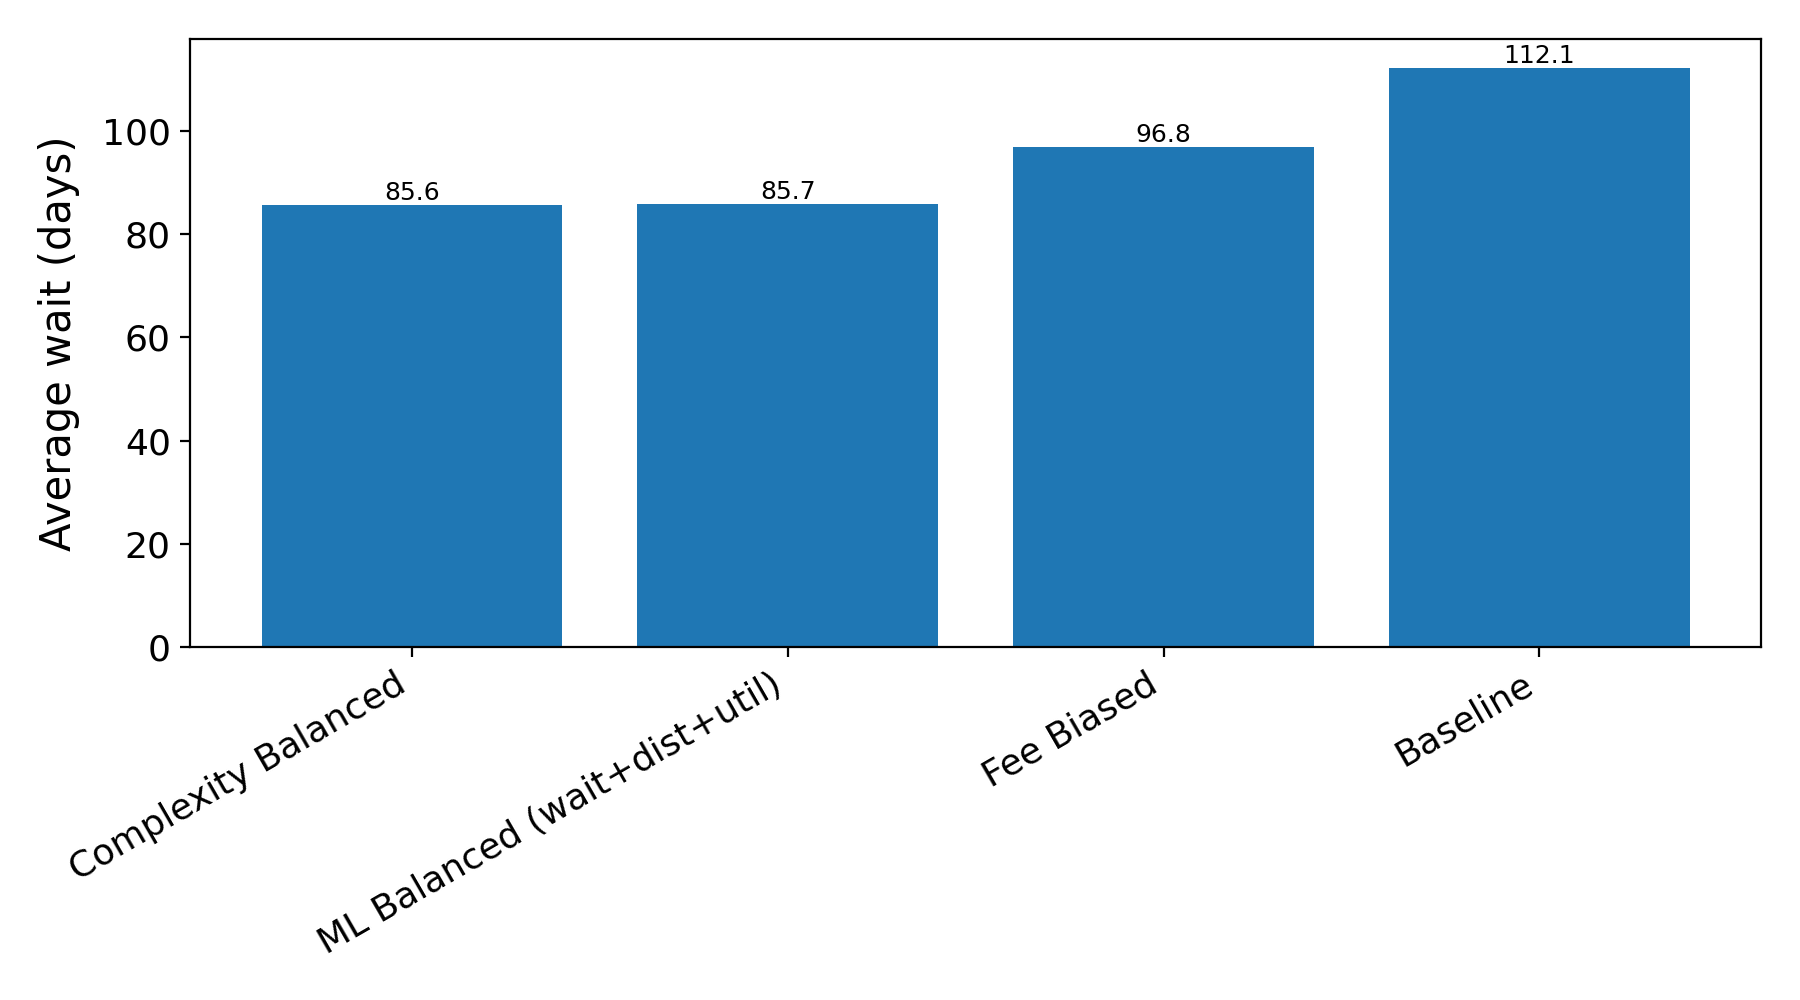
\includegraphics[width=0.87\linewidth]{fig/fig1_avg_wait_by_policy.png}
\caption{Average wait by policy.}
\label{fig:avg-wait}
\end{figure}

\clearpage
\begin{figure}[htbp]
\centering
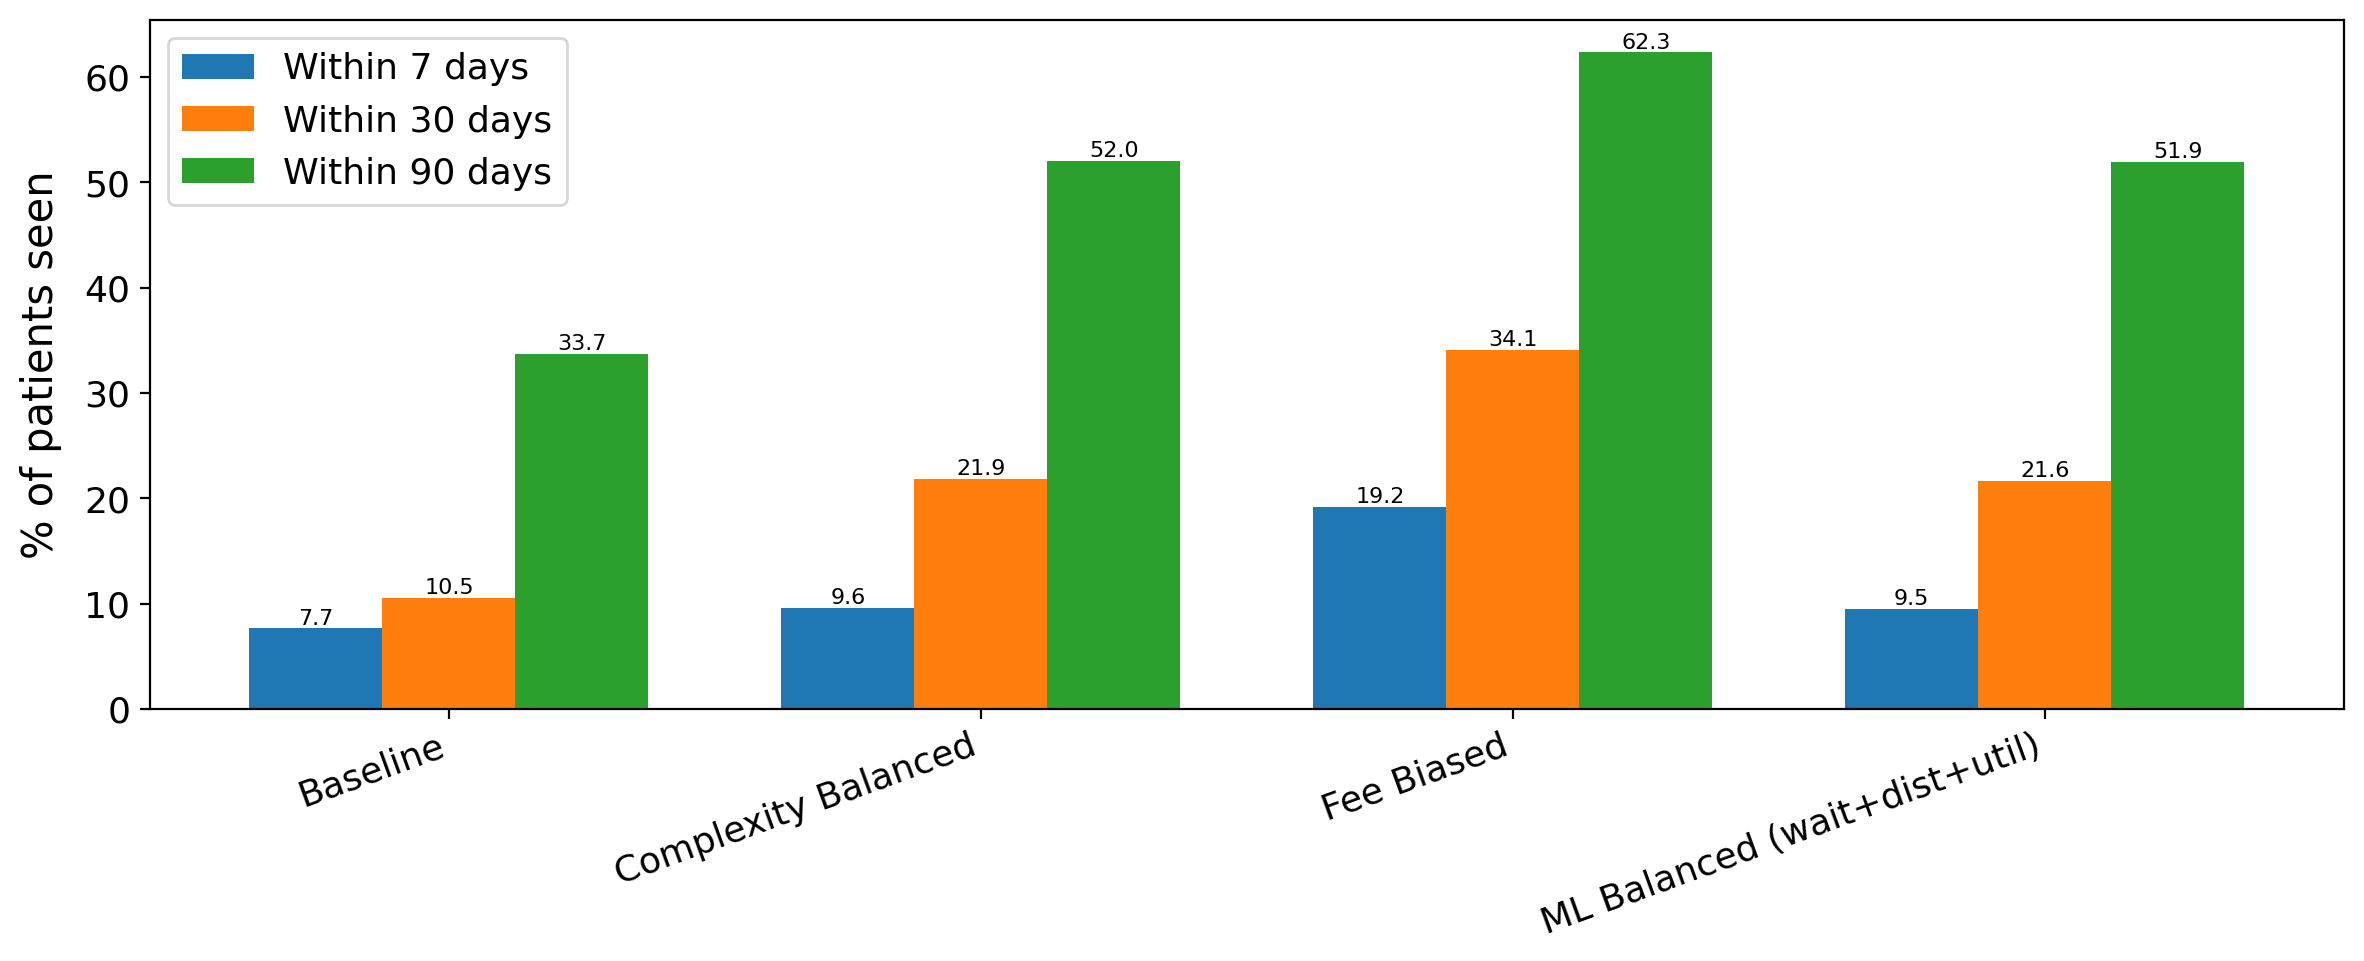
\includegraphics[width=0.85\linewidth]{fig/fig6a_seen_within.png}
\caption{\% patients seen within 7/30/90 days.}
\label{fig:pct-see}
\end{figure}

\paragraph{System efficiency vs NHS share (Figure~\ref{fig:wait-time-share}).}
Across policies, a higher NHS share is associated with longer waits (e.g., \textit{Baseline} $\approx$61\% NHS, $\sim$112 days; \textit{ML Balanced} $\approx$48\%, $\sim$86 days). To test for a single “sweet spot”, we swept the \emph{overall} NHS share from 30–90\% ($r=10$) under the same arrivals, capacity, and GA$\rightarrow$NHS rule. The waiting-time curve is flat across the mid-range (overlapping 95\% CIs), so no unique optimum emerges. This is consistent with two constraints: GA$\rightarrow$NHS sets a floor under NHS activity, and Independent capacity does not bind in this range. Adjusting the overall NHS share alone has limited impact. In practice, improvements only emerge when such adjustments are combined with complexity-aware allocation (see Appendix~\ref{fig:high-to-private-sensitivity} for the full sensitivity sweep).

\paragraph{Efficiency vs. patient burden (Figure~\ref{fig:tradeoff-wait}).} 
\textit{ML Balanced} and \textit{Complexity Balanced} achieve shortest wait while keeping travel distance comparable to other policies. \textit{Fee-biased} shows slightly shorter distance but longer wait than \textit{ML/Complexity}. \textit{Baseline} combines is both long wait without meaningful distance advantage. This indicates waiting-time reduction are achievable without a increasing travel-distance.

\begin{table}[htbp]
\centering
\footnotesize
\setlength{\tabcolsep}{4pt}
\begin{adjustbox}{width=\linewidth}
\begin{tabular}{lccccc}
\toprule
\textbf{Policy} & \textbf{Mean wait (d)} & \textbf{Seen$\le$7d (\%)} &
\textbf{Seen$\le$30d (\%)} & \textbf{Seen$\le$90d (\%)} & \textbf{Mean dist (km)} \\
\midrule
Baseline & 112.07 $\pm$ 0.16 & 7.73 $\pm$ 0.00 & 10.52 $\pm$ 0.01 & 33.71 $\pm$ 0.01 & 58.40 $\pm$ 0.02 \\
Complexity Balanced & 85.76 $\pm$ 0.08 & 9.59 $\pm$ 0.00 & 21.85 $\pm$ 0.01 & 52.05 $\pm$ 0.01 & 59.32 $\pm$ 0.03 \\
Fee Biased & 96.80 $\pm$ 0.09 & 19.20 $\pm$ 0.01 & 34.07 $\pm$ 0.01 & 62.34 $\pm$ 0.01 & 55.51 $\pm$ 0.03 \\
ML Balanced (wait+dist+util) & 85.71 $\pm$ 0.08 & 9.53 $\pm$ 0.01 & 21.64 $\pm$ 0.01 & 51.93 $\pm$ 0.01 & 57.61 $\pm$ 0.04 \\
\bottomrule
\end{tabular}
\end{adjustbox}
\caption{System-wide KPIs by policy (mean $\pm$ 95\% CI; $r=10$).}
\label{tab:sys-kpi-ci}
\end{table}

\begin{figure}[htbp]
\centering
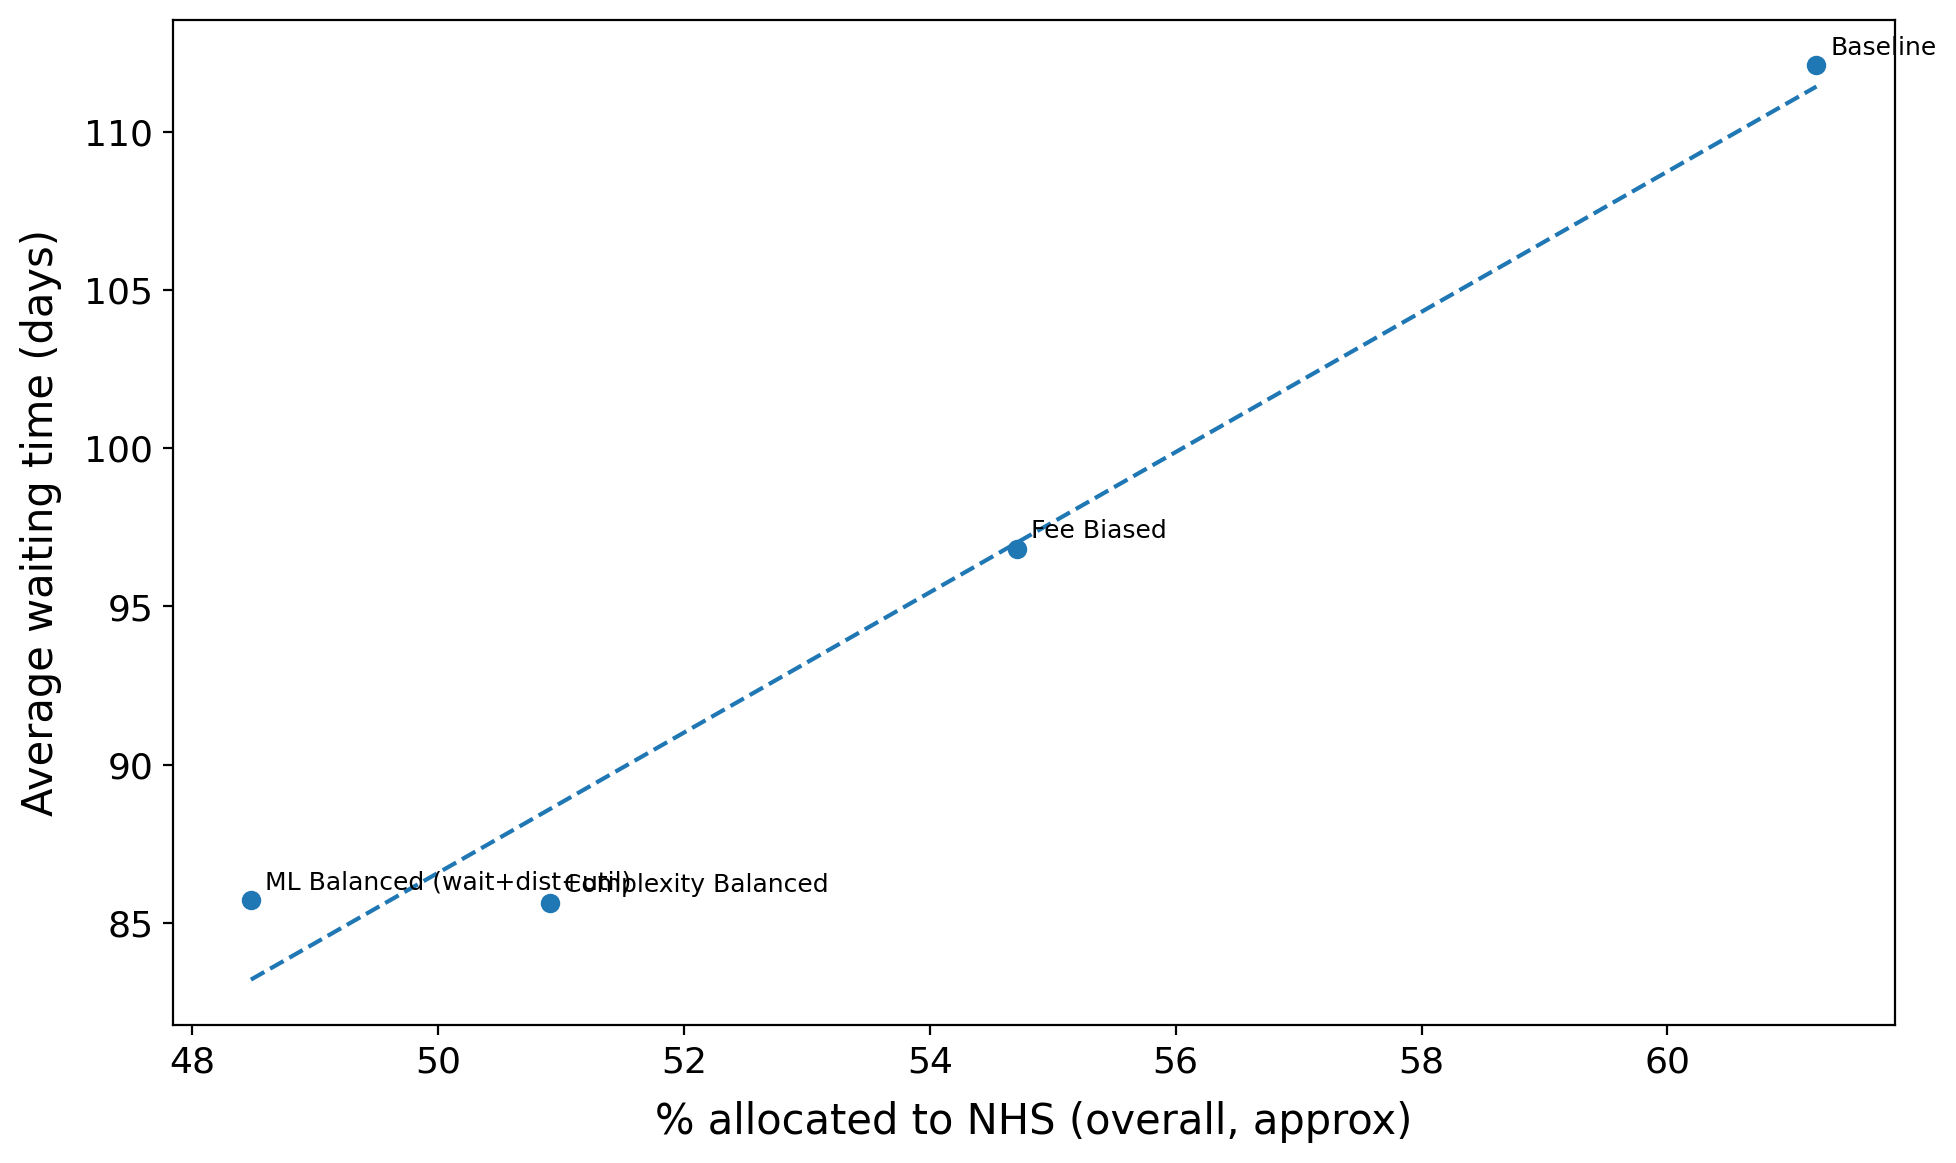
\includegraphics[width=0.7\linewidth]{fig/fig_wait_vs_nhs_share.png}
\caption{Waiting time vs NHS share.}
\label{fig:wait-time-share}
\end{figure}

\clearpage
\begin{figure}[htbp]
\centering
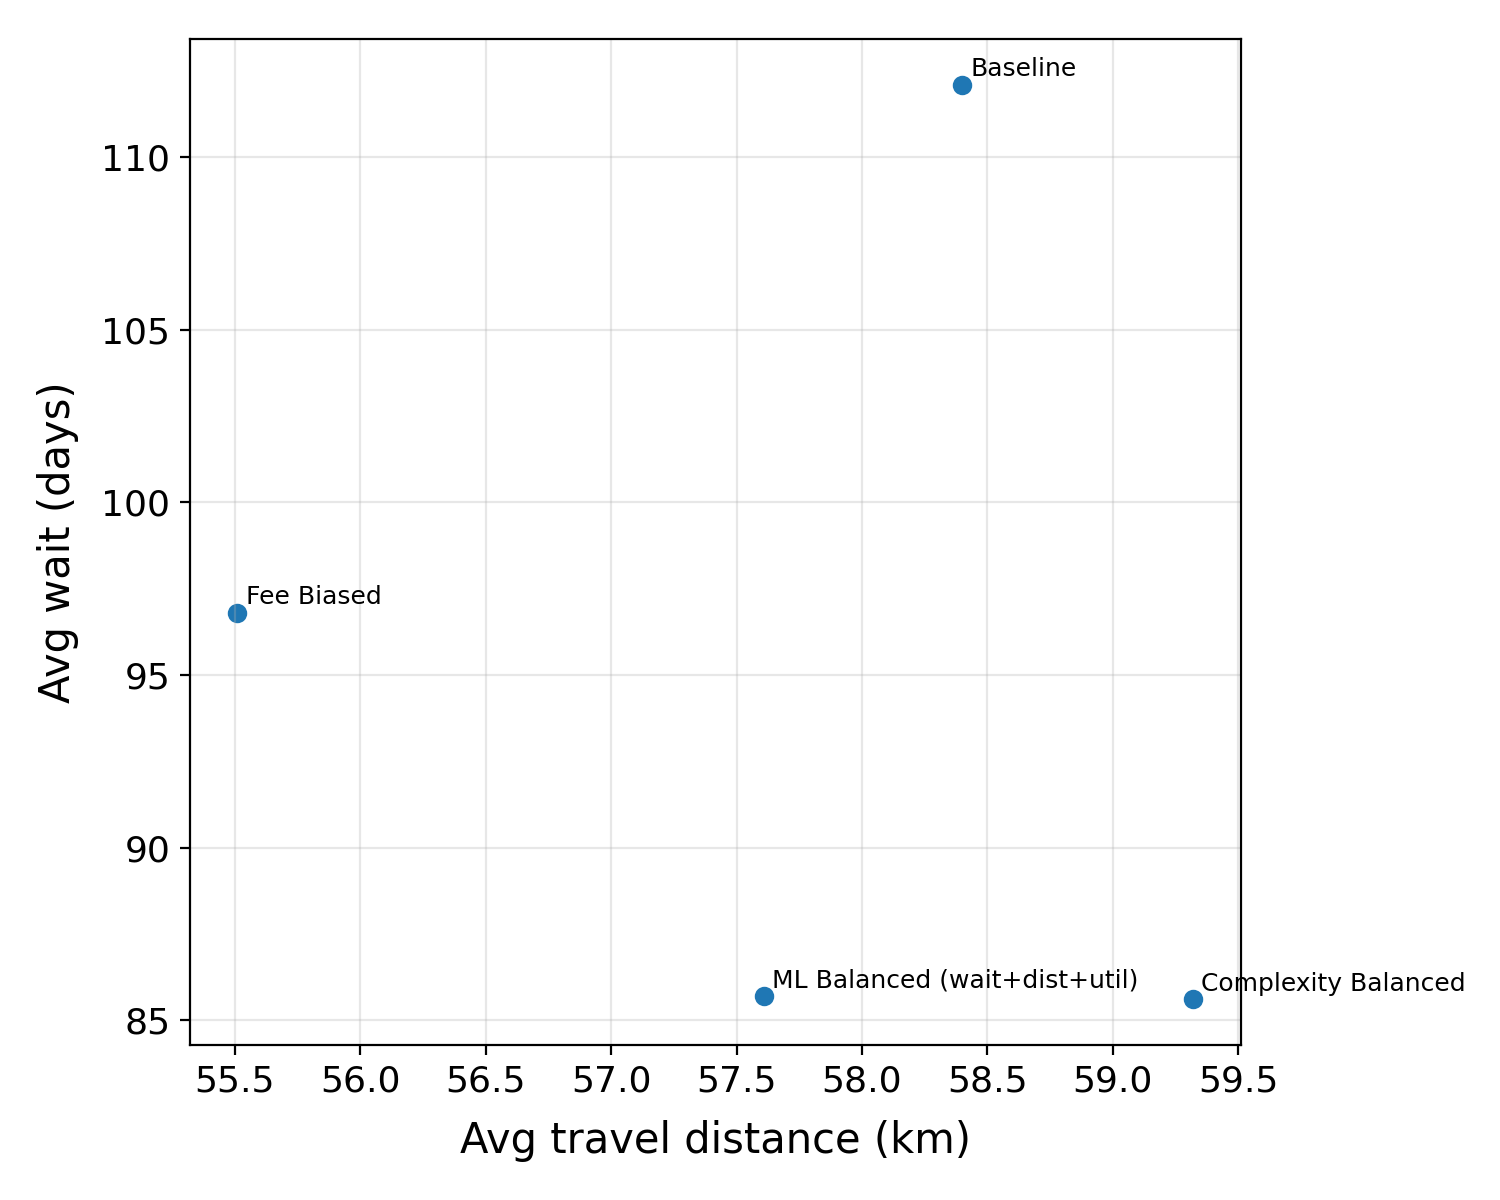
\includegraphics[width=0.77\linewidth]{fig/fig3_tradeoff_wait_vs_distance.png}
    \caption{Efficiency vs patient burden by policy.}
    \label{fig:tradeoff-wait}
\end{figure}

\paragraph{Summary}
Policies that rebalanced workload across sectors while respecting complexity, (\textit{ML Balanced} and \textit{Complexity Balanced}) reduce mean waits by $\sim$23-24\% compared with \textit{Baseline} (from $\sim$112 days to $\sim$85-86 days), without increasing travel burden (57.6-59.5 km vs 58.4 km) and also improves seen-within rates (Figure~\ref{fig:pct-see}). \textit{Fee-biased} improves some attainment metrics but raises incentive and case distribution. The NHS-share frontier (Figure~\ref{fig:wait-time-share}) clarifies that, under current capacity, pushing a higher NHS share tends to raise waits, while a more balanced split can help particularly when combined with complexity-aware allocation.


\section{Patient-level & Fairness}
\label{sec:patient-lev}
This section asks \emph{who gets what, when and where}, focus on differences between patient groups (Low/Medium/High complexity and GA/Non-GA status), as well as equity between NHS and Independent sector.

\paragraph{Case-mix and incentive (Table~\ref{tab:tariff-by-policy}, Figure~\ref{fig:comp-mix}--\ref{fig:avg-tariff-sector}).}
\textit{ML Balanced} and \textit{Complexity Balanced} reduce bottleneck by shifting some complex case to Independent, clearing the queue overall. In contrast, \textit{Fee-biased} shows stronger return-based selection and consistent with higher average tariff in the Independent sector ($\approx$£830 for Fee-biased) compared with Baseline ($\approx$£748) and ML/Complexity ($\approx$£797–£800). These values are computed from the HRG schedule in Table~\ref{tab:tariff} by weighting each HRG tariff with the observed case-mix assigned to the Independent sector. 

Figure~\ref{fig:comp-mix} shows how policies reallocates Low/Med/High cases between NHS and the Independent sector. Figure~\ref{fig:avg-tariff-sector} shows the average HRG-weighted tariff by sector. In our model, both sectors are using the same HRG tariff schedule (Table~\ref{tab:tariff}). So the average \pounds \hspace{0.1cm} per case mainly reflect case-mix, not price differences. Under Fee-biased, more higher-tariff HRGs move to the Independent sector, which raises \textit{Avg $\pounds$ Ind.} (Table~\ref{tab:tariff-by-policy}), and at the same time GA cases and more complex work remain in NHS by rule (GA$\rightarrow$NHS), which can lift  \textit{Avg \pounds{} NHS}. This pattern raises two equity concern: 

\begin{enumerate}
    \item Selection of higher-return cases into the Independent sector.
    \item A heavier case-mix (and potential budget/queue pressure) left with the NHS.
\end{enumerate}

\begin{table}[htbp]
\centering
\small
\setlength{\tabcolsep}{5pt}
\renewcommand{\arraystretch}{1.10}
\begin{adjustbox}{width=\linewidth}
\begin{tabular}{lrrrrrrr}
\toprule
\textbf{Policy} & \textbf{Unassigned} & \textbf{Total £ (all)} &
\textbf{Total £ NHS} & \textbf{Total £ Ind.} & \textbf{Avg £/case} &
\textbf{Avg £ NHS} & \textbf{Avg £ Ind.} \\
\midrule
Baseline & 707 & 27{,}350{,}040 & 15{,}244{,}895 & 12{,}105{,}145 & 801.21 & 848.68 & 748.48 \\
Complexity Balanced & 0 & 27{,}919{,}230 & 14{,}219{,}052 & 13{,}700{,}178 & 801.29 & 802.75 & 799.78 \\
Fee Biased & 2{,}219 & 27{,}417{,}550 & 12{,}117{,}302 & 15{,}300{,}248 & 840.41 & 854.29 & 829.73 \\
ML Balanced (wait+dist+util) & 0 & 27{,}919{,}230 & 13{,}590{,}487 & 14{,}328{,}743 & 801.29 & 805.60 & 797.24 \\
\bottomrule
\end{tabular}
\end{adjustbox}
\caption{HRG-weighted spend and average tariff per treated case by sector.}
\label{tab:tariff-by-policy}
\end{table}

\begin{figure}[htbp]
\centering
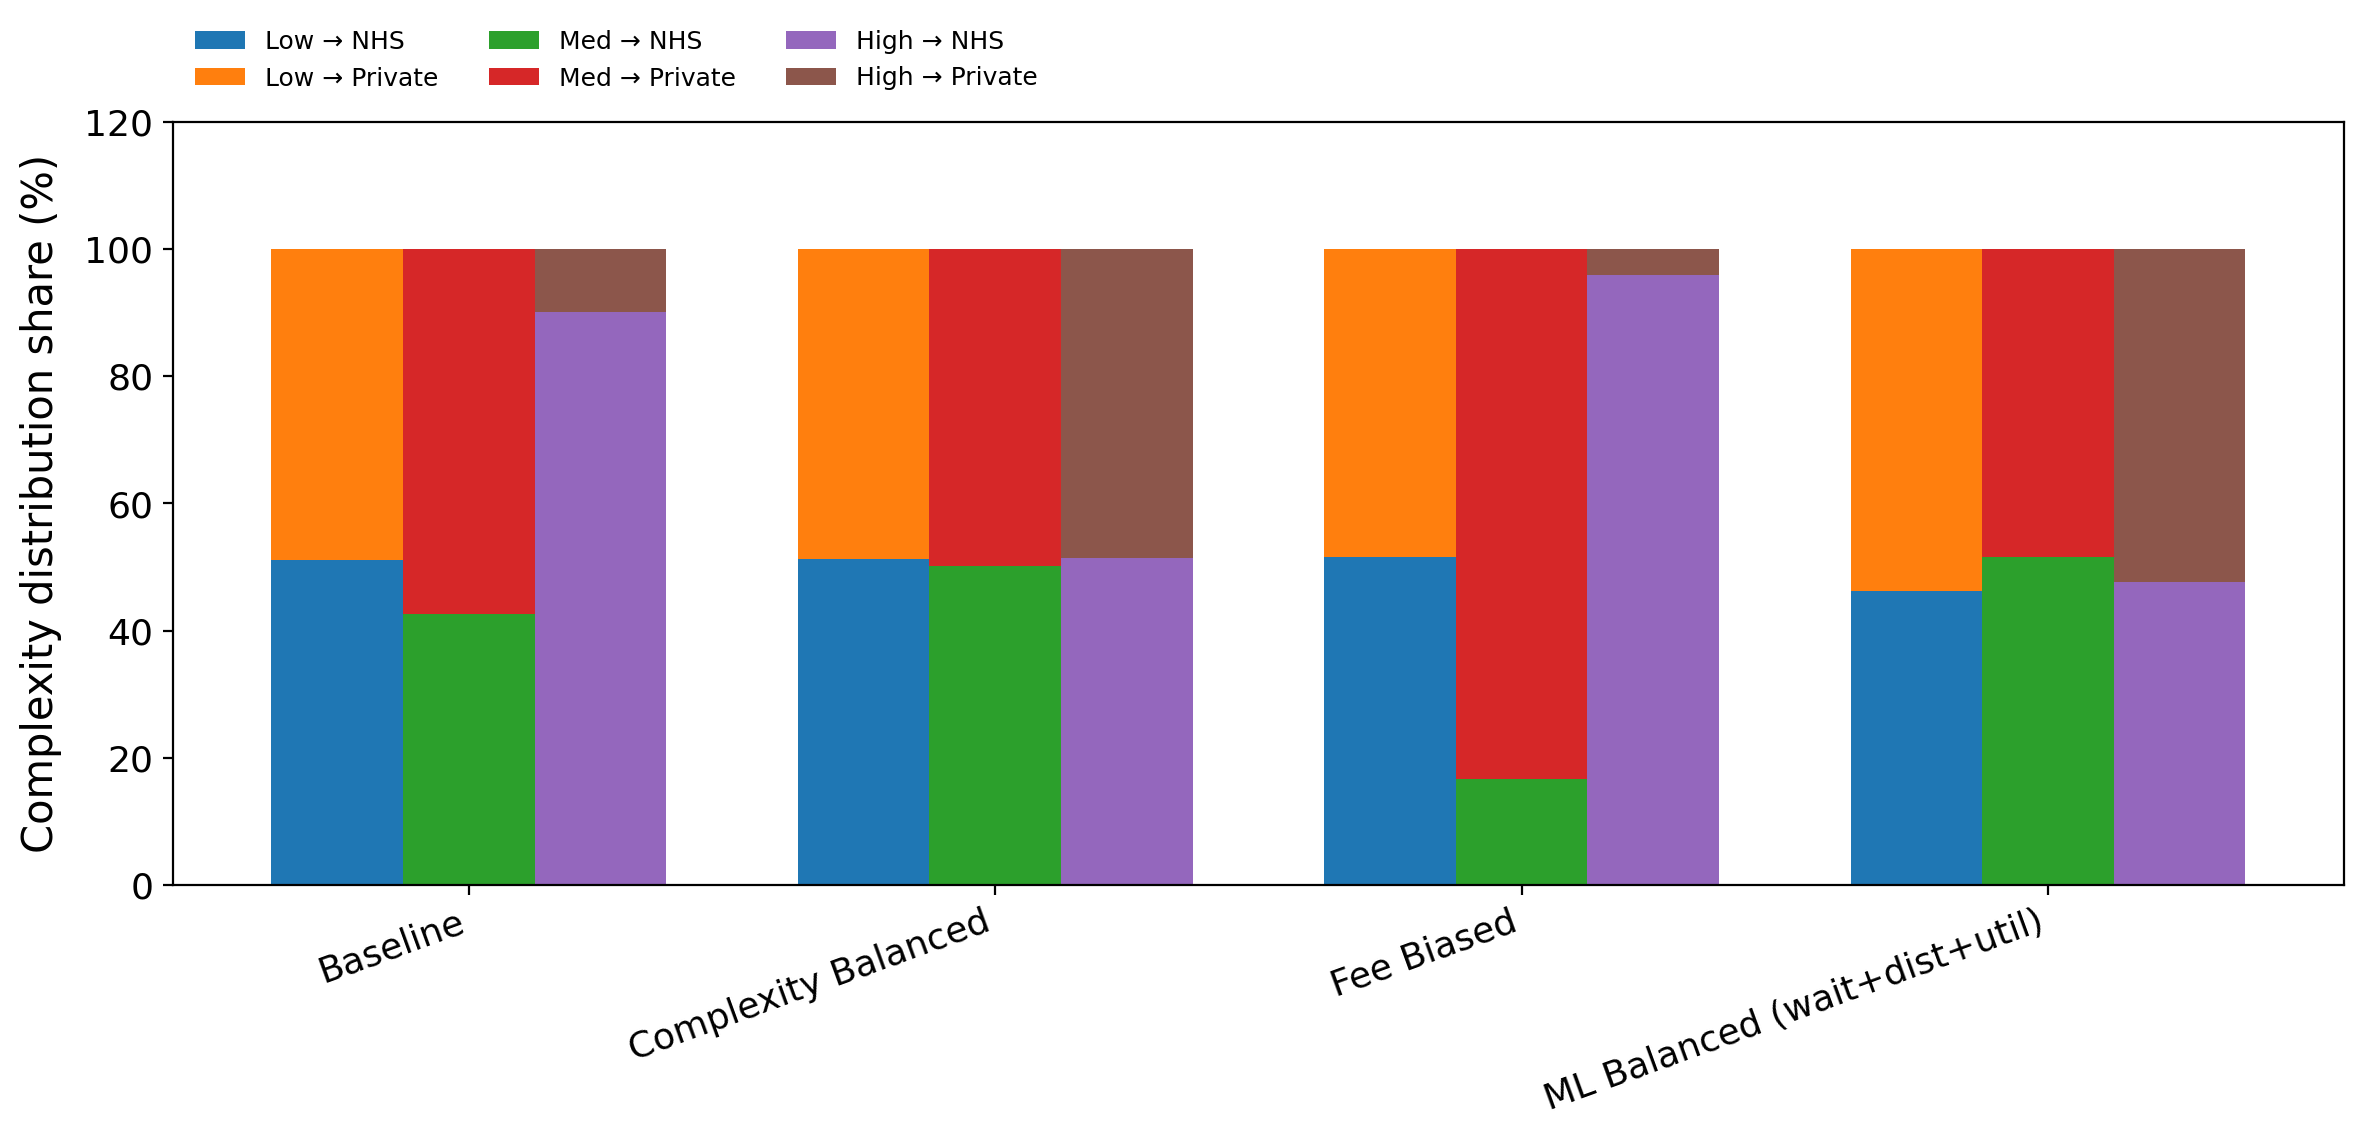
\includegraphics[width=0.92\linewidth]{fig/fig5a_complexity_mix_by_group.png}
\caption{Complexity mix by sector (NHS vs Independent).}
\label{fig:comp-mix}
\end{figure}

\begin{figure}[htbp]
\centering
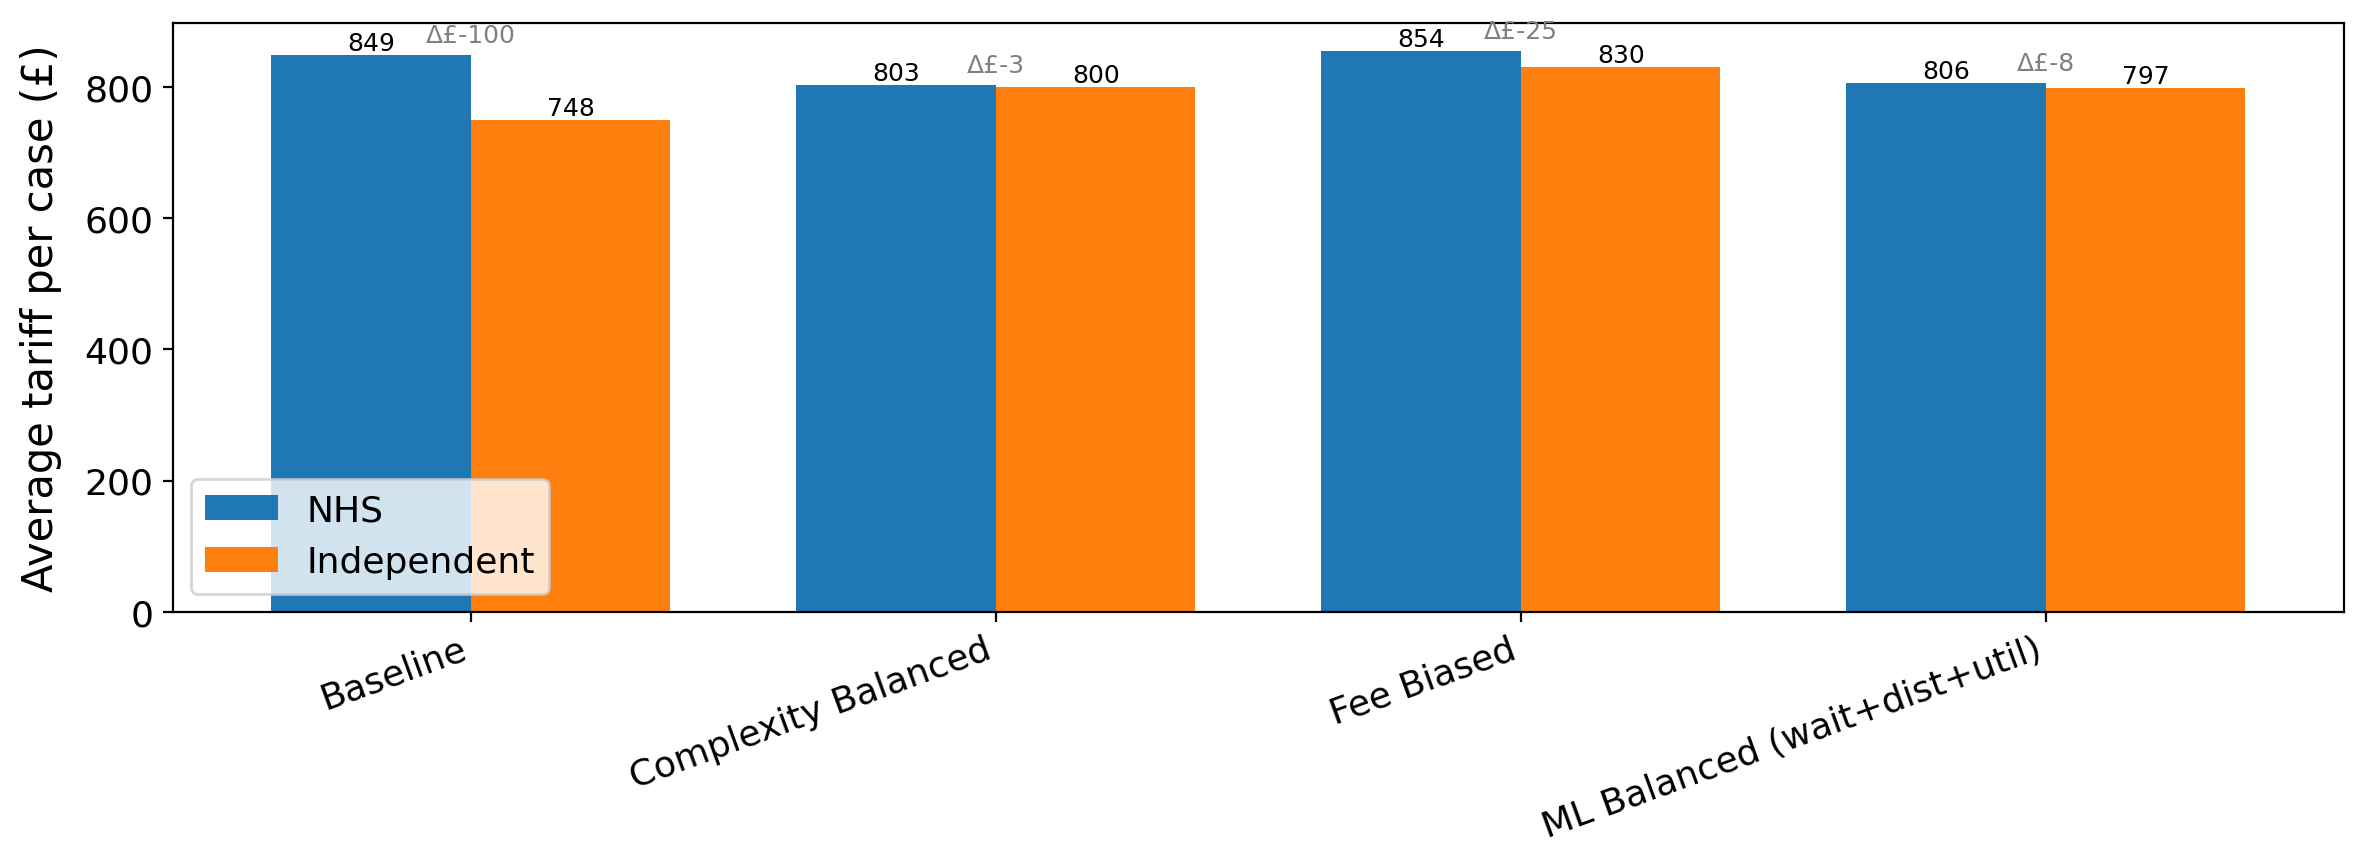
\includegraphics[width=0.92\linewidth]{fig/fig5b_avg_tariff_by_sector.png}
\caption{Average HRG-weighted tariff per treated case by sector (NHS vs Independent).}
\label{fig:avg-tariff-sector}
\end{figure}

\paragraph{Complexity differences (Figure~\ref{fig:avg-wait-by-comp}).} \textit{ML Balanced} and \textit{Complexity Balanced} compress a gap across complexity level (Low/Med/High at $\sim$84-88 days). In contrast, \textit{Fee-biased} creates clear inequality (Low $\sim$167 days; Medium 40; High $\sim$16 days), consistent with tariff-driven selection: high-return cases are pulled quickly to Independent while other group wait longer in NHS.

\begin{figure}[htbp]
\centering
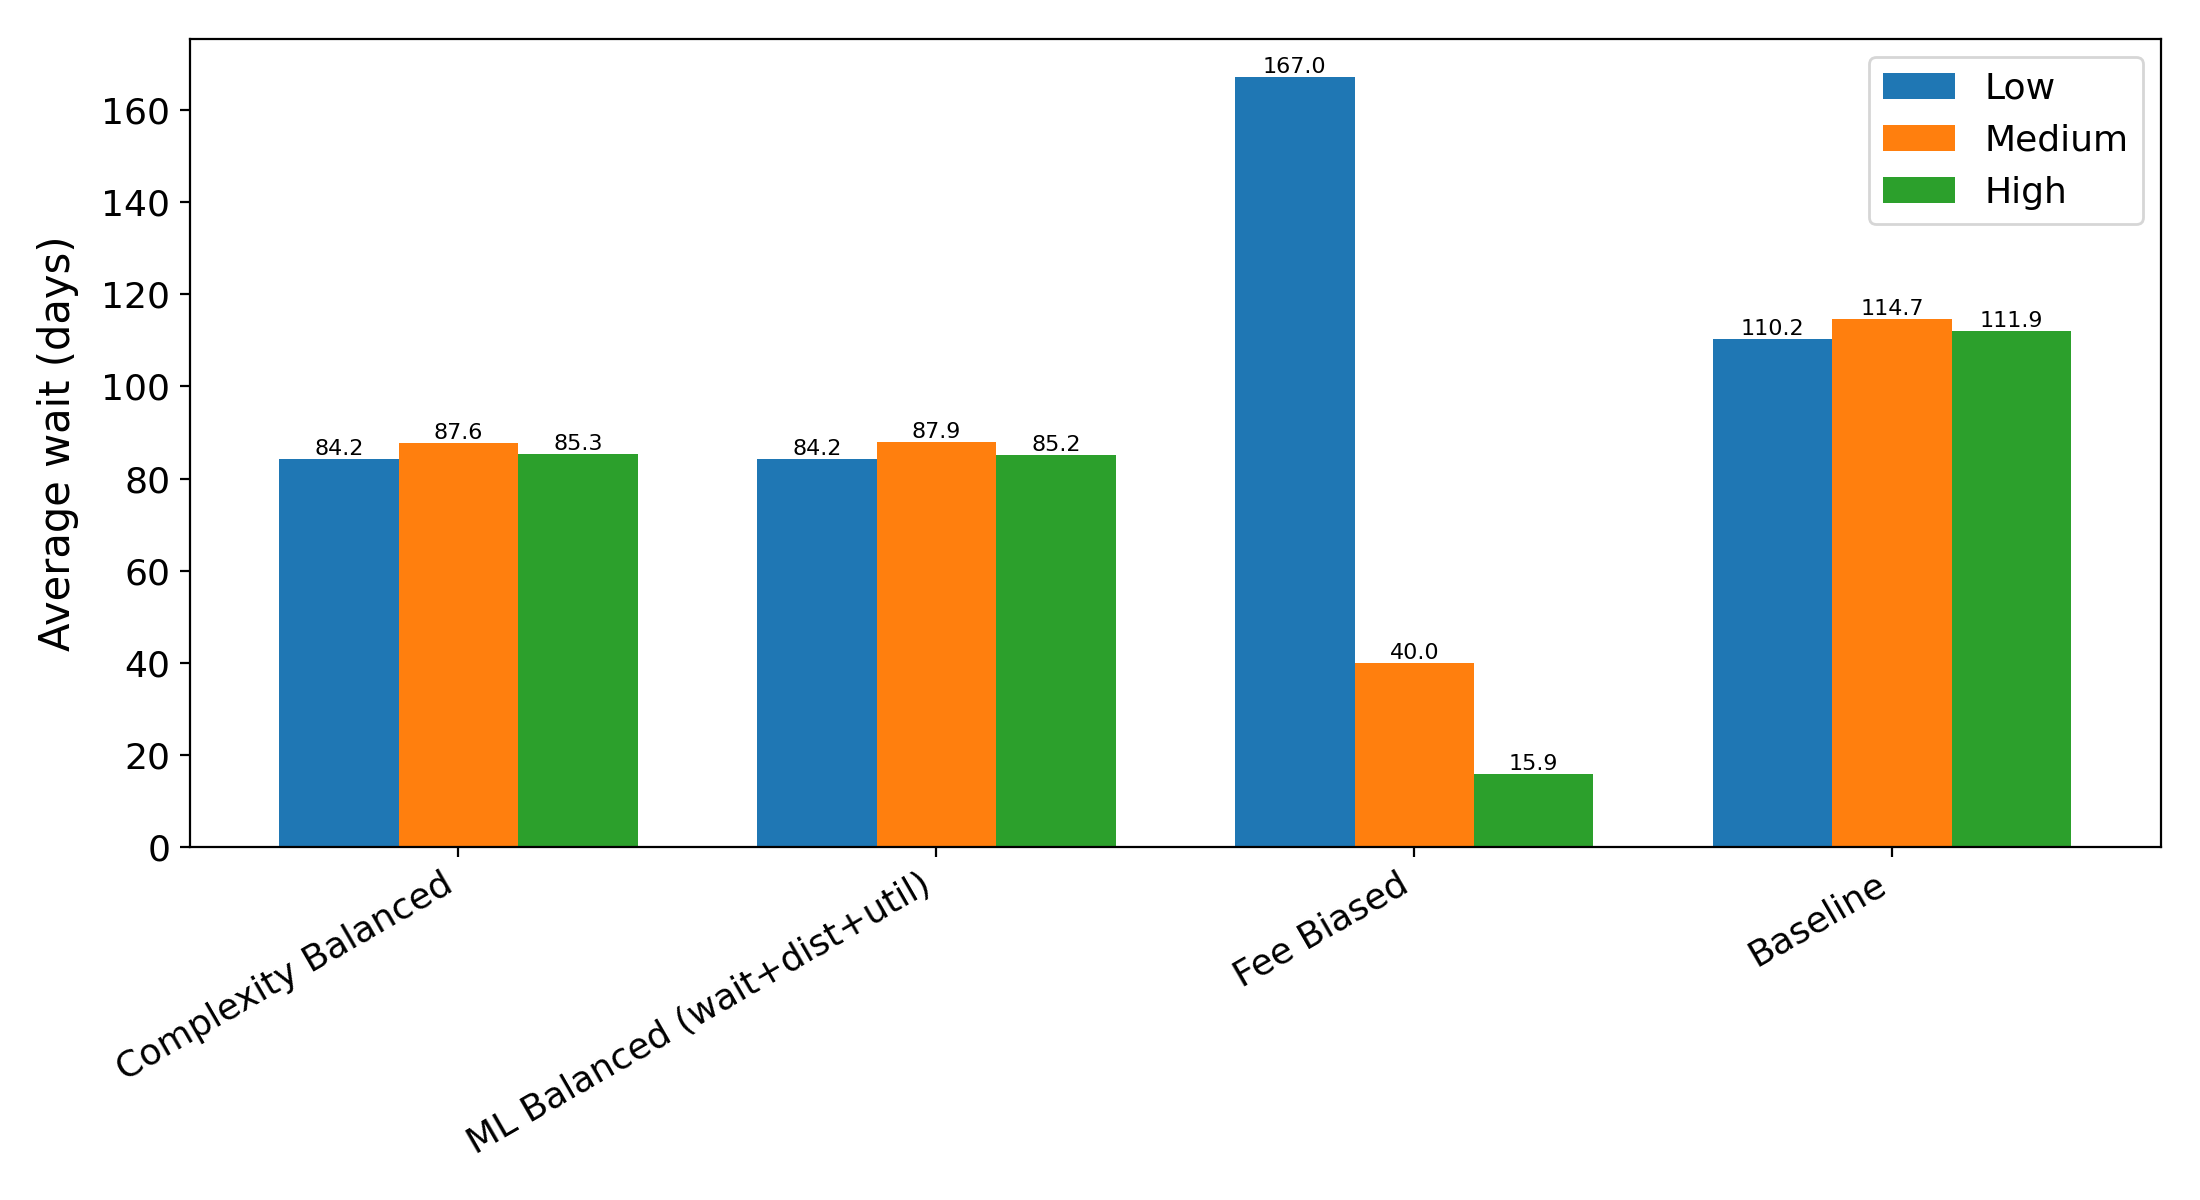
\includegraphics[width=0.92\linewidth]{fig/fig4_wait_by_complexity.png}
\caption{Average wait by complexity and policy.}
\label{fig:avg-wait-by-comp}
\end{figure}

\begin{figure}[htbp]
\centering
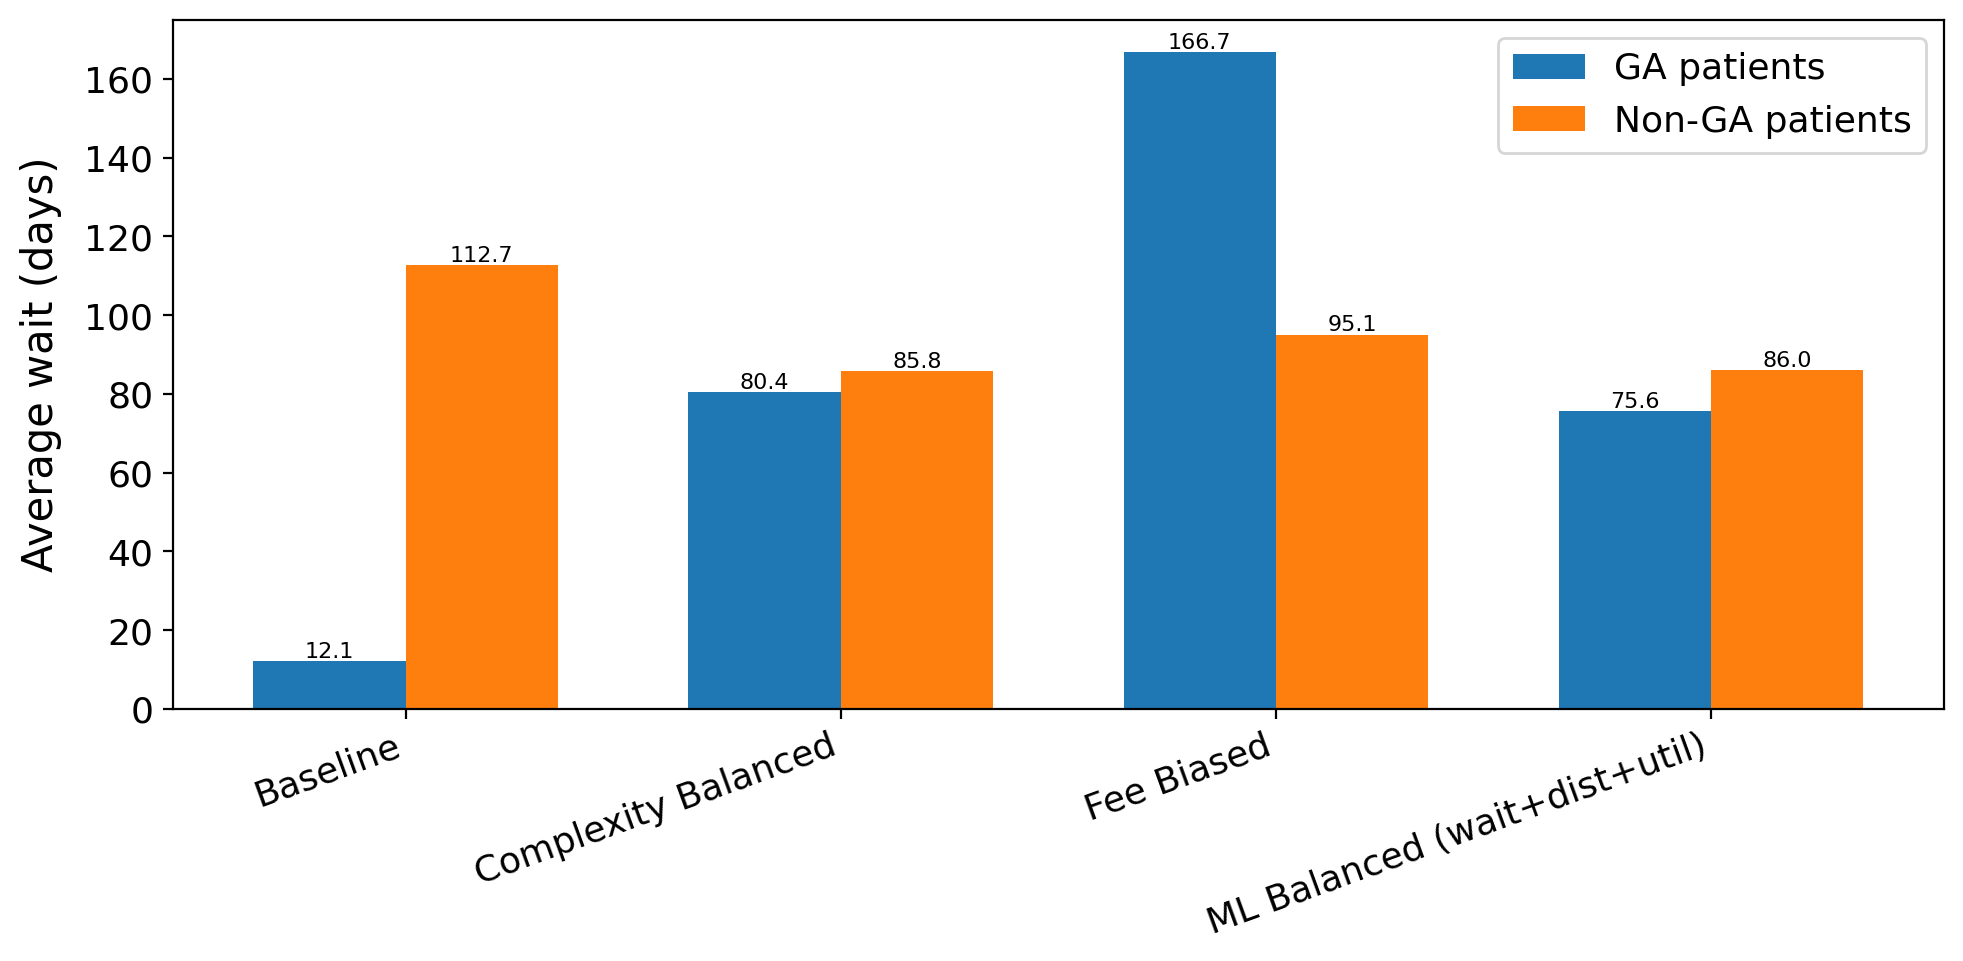
\includegraphics[width=0.92\linewidth]{fig/fig6b_wait_ga_vs_non_ga.png}
\caption{Average wait: GA vs Non-GA by policy.}
\label{fig:ga-non-ga}
\end{figure}

\paragraph{Summary}
At the patient level, \textit{ML Balanced} and \textit{Complexity Balanced} narrow inequities across complexity and GA status (Figure~\ref{fig:ga-non-ga}) while keeping travel comparable to \textit{Baseline}. \textit{Fee-biased} improves some attainment metrics but introduces inequities between group gaps and raises average private tariff (Figures~\ref{fig:comp-mix}–\ref{fig:avg-tariff-sector}). On our data, the Independent average is \emph{not} uniformly higher: it rises mainly under \textit{Fee-biased} because the case-mix shifts toward higher-tariff HRGs (e.g. BZ30A/BZ34A in Table~\ref{tab:tariff}). Under \textit{ML Balanced} and \textit{Complexity Balanced}, the Independent average stay closer to the system average because case-mix is more even across sectors. If equity and shorter queues are the objectives, \textit{ML/Complexity} dominate, while \textit{Fee-biased} is better used as an incentive stress test. These patterns are consistent with the system-wide results: allowing Independent capacity to absorb bottlenecks reduces waits across complexity (Figure~\ref{fig:avg-wait}) while keeping NHS/Independent shares balanced (Figure~\ref{fig:comp-mix}).


\subsection{Evaluation of ML models for provider ranking}
We evaluate the ranking model against an oracle that knows the truly fastest provider per case. This section has two parts: (a) a micro-level \emph{offline} test of the model's ability to rank providers, and (b) a full \emph{online} simulation where the model is embedded in the allocation policy.

\emph{(a) Offline micro-evaluation.} 
Here we test whether the model can place the oracle provider near the top of ranking list. Hit@$k$ measures how often the oracle provider appears within the model's top $k$ choices, and MRR@$k$ captures the average position (higher=better). Results show Hit@1 $=0.275$, Hit@3 $=0.525$, and MRR@3 $=0.457$, meaning the oracle tends to sit around rank 2-3 rather than rank 1. If we simply pick the top-1 prediction and fall back within the top-3 with limited lookahead, the average predicted wait is 10.22 days. For comparison, an oracle that always picks the fastest available option achieves 6.90 days, so the performance gap is about 3.3 days.

\emph{(b) Online policy in the loop.}
The offline test ignores system-wide effects such as daily capacity, backlog, and clinical constraints. To address this, we embed the model inside the \texttt{ml\_balanced\_policy} and simulate over a full year. Under these dynamics (365 days of arrivals, GA$\rightarrow$NHS rule, sectoral service times, etc.), the policy achieves an overall mean wait of 85.71 days (Table~\ref{tab:sys-kpi-ci}). This is better than the baseline but still above the oracle lower bound.

\paragraph{Why ML is still below the oracle.} 
Three main factors explain the gap:
\begin{enumerate}
    \item \textbf{Ranking quality:} Hit/MRR results show the model often places the oracle provider at rank 2-3, so "pick top-1" miss the fastest choice.
    \item \textbf{Search/availability limit:} A small \texttt{top\_k} and short \texttt{lookahead\_days}, plus duplicate booking make the predicted-fast slot can be unavailable on the decision day. 
    \item \textbf{Multi-objective scoring:} The policy balances predicted wait against travel distance and utilization $(\lambda_d,\lambda_u)$, and service time depends on complexity$\times$sector. As a result, the "expected fastest" option is not always chosen in practice under real bottlenecks.
\end{enumerate}

\paragraph{Summary}
The offline evaluation shows the ML model typically ranks the true best provider around 2-3 rather than 1 (Hit@1 $=0.275$, Hit@3 $=0.525$, and MRR@3 $=0.457$). This produces an average predicted wait of 10.22 days, about 3.3 days above the oracle. Once embedded in policy and simulated with system dynamics, the model achieves a mean wait of 85.71 days. Further improvements will require raising Hit@1, incorporating availability-aware features to reduce booking collisions, and tuning $(\lambda_d,\lambda_u,\texttt{top\_k},\texttt{lookahead\_days})$ to balance to balance deeper search with runtime.

\begin{table}[htbp]
\centering
\small
\begin{tabular}{l c l}
\toprule
\textbf{Metric} & \textbf{Value} & \textbf{Interpretation} \\
\midrule
Hit@1 & 0.275 & Proportion of cases that the model places oracle at first \\
Hit@3 & 0.525 & Proportion of case that the model places oracle at 1–3 \\
MRR@3 & 0.457 & Average rank of oracle around 2–3 \\
\midrule
Best possible avg wait (oracle) & 6.90 days & Choose the fastest service provider based on past performance. \\
ML Top-3 + fallback avg & 10.22 days & Select rank 1; If it doesn't work, try it inside. Top-3 and lookahead \\
$\Delta$ wait (ML - Best) & 3.32 day & ML performance gap with ideal lower bound \\
\bottomrule
\end{tabular}
\caption{The quality of ML model ranking and its impact on average waiting time}
\label{tab:ml-metrics}
\end{table}

\paragraph{Evaluation caveat.}
The results in this chapter rely on specific modeling assumptions and scope (e.g., daily capacity, GA$\rightarrow$NHS clinical rule, and service time approximated by complexity$\times$sector averages). These results should be read alongside the detailed discussion of limitations and policy implications in Chapter~\ref{chap:conclusion}, Section~\ref{sec:limits-imp}.


% -----------------------------------------------------------------------------

\chapter{Conclusion}
\label{chap:conclusion}

This chapter summarizes the main contribution, evaluates progress against the initial objective, revisits the research question, and identify the limitation, implication, and future work. Unless noted otherwise, summaries refer to the 365-day experiments with fixed \emph{arrival} and \emph{capacity} streams and the policy settings defined in Chapter~\ref{chap:execution}.

\section{Contributions and Achievements}
This project delivers:
\begin{enumerate}
    \item Single patient waiting-list simulation architecture at the \emph{patient} and \emph{provider} levels with clinical constrain (e.g. GA$\rightarrow$NHS).
    \item A comparison of allocation policies (Baseline, Complexity/ML Balanced, Fee-biased, etc.) under the same condition.
    \item Evaluation of system effectiveness and fairness, including an assessment of the ranking quality of the ML model used for provider selection. 
\end{enumerate}

\begin{table}[htbp]
\centering
\small
\renewcommand{\arraystretch}{1.15}
\begin{tabularx}{\linewidth}{@{} p{3.8cm} X p{3.2cm} @{}}
\toprule
\textbf{Objective} & \textbf{Evidence \& Reference} & \textbf{Status} \\
\midrule
Develop tool to simulate clinical constraints (GA$\rightarrow$NHS) and daily capacity
& Chapter~\ref{chap:execution}; Algorithm~\ref{alg:runner}; Tables~\ref{tab:log-patient}, \ref{tab:log-provider-day}
& Completed \\
Define/test multiple allocation policies under identical streams
& Chapter~\ref{chap:evaluation}, Section~\ref{sec:sys-wide}; Figures~\ref{fig:avg-wait}--\ref{fig:pct-see}; Table~\ref{tab:sys-kpi-ci}
& Completed \\
Evaluate equity by complexity group and GA/Non-GA
& Section~\ref{sec:patient-lev}; Figures~\ref{fig:avg-wait-by-comp}, \ref{fig:ga-non-ga}
& Completed \\
Create/test ML model for provider ranking
& Chapter~\ref{chap:evaluation} (ML evaluation); Table~\ref{tab:ml-metrics}
& Completed (quality below ideal) \\
Synthesize policy implications from simulation results
& Chapter~\ref{chap:conclusion}, Section~\ref{sec:limits-imp}
& Completed \\
\bottomrule
\end{tabularx}
\caption{Initial objectives, evidence, and completion status.}
\label{tab:aims-status}
\end{table}

\section{Synthesis of Findings}
System-wide, rebalancing workload across sectors with complexity awareness reduces mean waits and raises seen-within rates without a distance penalty (Figures~\ref{fig:avg-wait}, \ref{fig:tradeoff-wait}; Table~\ref{tab:sys-kpi-ci}). The NHS-share frontier indicates that, under current capacity, pushing a higher NHS share increases waits (Figure~\ref{fig:wait-time-share}). At the patient level, \textit{ML/Complexity} compress gaps across complexity and GA status (Figures~\ref{fig:avg-wait-by-comp}, \ref{fig:ga-non-ga}); \textit{Fee-biased} boosts some KPIs but aligns with higher average private tariff (Figure~\ref{fig:avg-tariff-sector}) and wider between group gap. The ML ranking model improves system outcomes when embedded in policy (85.71 days on average). However, it remains below an oracle's lower bound due to ranking error and limited feature availability (Table~\ref{tab:ml-metrics}). 

\paragraph{On the NHS-Independent balance}
Across a sweep of 30-90\% NHS share, the waiting-time curve is broadly flat in the mid-range and no unique optimum emerges . This reflects two constrains: the GA$\rightarrow$NHS rule sets a floor under NHS activity, and Independent capacity is not fully saturated. Under current conditions, therefore, simply shifting the NHS/Independent split does not provide a clear threshold or reversal. However, in alternative scenarios. For example if NHS capacity were expanded, or if Independent capacity were restricted we could expect the balance point to shift, and a genuine optimum might emerge. This suggests that capacity configuration, not share alone, determines whether a turning point exists (see Appendix~\ref{fig:high-to-private-sensitivity} for the full sensitivity sweep).

These finding highlight that observed trends are dependent on specific modeling assumptions (capacity, case-mix, clinical rules) and should be interpreted with caution. This issues are developed further in the following section on limitations and policy implications.

\section{Limitations of Results and Policy Implications}
\label{sec:limits-imp}
\paragraph{Limitation.} 
The observed flatness of the NHS/Independent frontier and related finding are contingent on specific modeling choices. Finding are specific to the cataract pathway and should not be generalized directly to other clinical specialties (e.g., oncology, orthopedics). This tool targets strategic planning, not real-time operations. Micro-events (day-specific cancellations), team logistics, and case-level service-time are simplified: \texttt{get\_service\_time()} uses complexity$\times$sector averages; some GA flags are imputed to preserve proportions. Patient selection behavior and fine-grained theatre logistics are not explicitly modeled.

\paragraph{Implications.}
These implication follow directly from the finding that rebalancing by complexity rather than altering the overall NHS/Independent split is the true lever for reducing waits. Using Independent capacity with clinical constrains (e.g., GA$\rightarrow$NHS; caps on High$\rightarrow$ Independent; utilization triggers) and complexity-aware balancing can reduce mean waits by $\sim$23\%, without increasing travel burden and with fewer unassigned cases. If \textit{Fee-biased} is considered operationally, fairness safeguards are needed (monthly case-mix monitoring, caps on average private tariff). For ML policies, further gains depend on better ranking (raise Hit@1), increasing availability features, and tuning $(\lambda_d,\lambda_u,\texttt{top\_k},\texttt{lookahead\_days})$ while keeping runtime tractable.

\section{Future Work}
The limitations above suggest several directions for extension.
\textbf{Improving the ML ranking and search logic.} Augment features with day-ahead availability signals (capacity shocks, booking collision risk), explore learning-to-rank objectives that support optimize wait, distance, and utilization, and adapt \texttt{top\_k}/\texttt{lookahead\_days} to context (e.g., deeper search only when predicted congestion is high).

\textbf{Operational realism.} Extend the model with cancellation/overrun processes, model theater team composition (anaesthesia, equipment/lens constraints), and allow shift rules across sites to capture realistic bottlenecks and backfill.

\textbf{Fairness and incentive.} Add fairness indicators (e.g., disparate impact by complexity/GA and geography), run sensitivity to the High$\rightarrow$Independent cap and tariff schedules, and quantify the budgetary impact of alternative incentive designs that preserve equity.

\section{Summary}

In short, the results answer the research questions directly. For the primary question—what a central allocation should look like. The evidence points to a cross-sector, complexity-aware allocator with clear clinical constraints (GA$\rightarrow$NHS and a cap on High$\rightarrow$Independent). Under like-for-like arrivals and capacity, this design consistently shortens waits (to $\sim$85–86 days from $\sim$112) without adding travel burden, and improves attainment within 7/30/90 days (see Chapter~\ref{chap:evaluation}). For the secondary questions, the NHS-share frontier and tariff patterns explain today’s imbalance: tight NHS capacity and incentive signals leave Independent capacity under-used, leading to longer waits. \textit{Complexity Balanced} and \textit{ML Balanced} policies rebalance by complexity and cut waits by $\sim$23–24\% with no distance penalty, while narrowing inequities across GA/non-GA and Low/Med/High groups and keeping complex work within NHS for training. ML helps when embedded in policy, but ranking quality and limited lookahead still leave a gap to the oracle; raising Hit@1 and improving availability awareness are the next levers.

These conclusions rely on comparisons designed to isolate policy logic from noise: all policies run on the same arrival and capacity streams, are repeated across seeds with 95\% CIs, and follow the same clinical rules. This design allow us to observe differences between the allocation policy. The findings do not rely on a single run or a favourable case-mix, but on consistent effects across settings.

Overall, this work delivers a policy simulation platform that makes trade-offs between waiting time, travel burden, fairness, and incentives transparent under real clinical constraints. Cross-sector, complexity-aware policies reduce queues without increasing travel. While \textit{ML Balanced} outperforms Baseline at the system level, ranking quality and limited lookahead leave room for improvement. Future work should deepen availability-aware ML and operational realism to support evidence-based decision-making with greater confidence.

% =============================================================================

% Finally, after the main matter, the back matter is specified.  This is
% typically populated with just the bibliography.  LaTeX deals with these
% in one of two ways, namely
%
% - inline, which roughly means the author specifies entries using the 
%   \bibitem macro and typesets them manually, or
% - using BiBTeX, which means entries are contained in a separate file
%   (which is essentially a database) then imported; this is the 
%   approach used below, with the databased being dissertation.bib.
%
% Either way, the each entry has a key (or identifier) which can be used
% in the main matter to cite it, e.g., \cite{X}, \cite[Chapter 2}{Y}.

\backmatter

\bibliographystyle{plain}
\bibliography{references}

% -----------------------------------------------------------------------------

\appendix
\chapter{Appendix}
\label{appx:example}

\section{Github Repository}
Github Repo: \href{http://www.github.com/nattanan267/dsp-257997}{Link} 

\section{Policy Supplement}
\label{app:policy-supplement}


\begin{figure}[htbp]
  \centering
  \begin{subfigure}{0.43\linewidth}
    \centering
    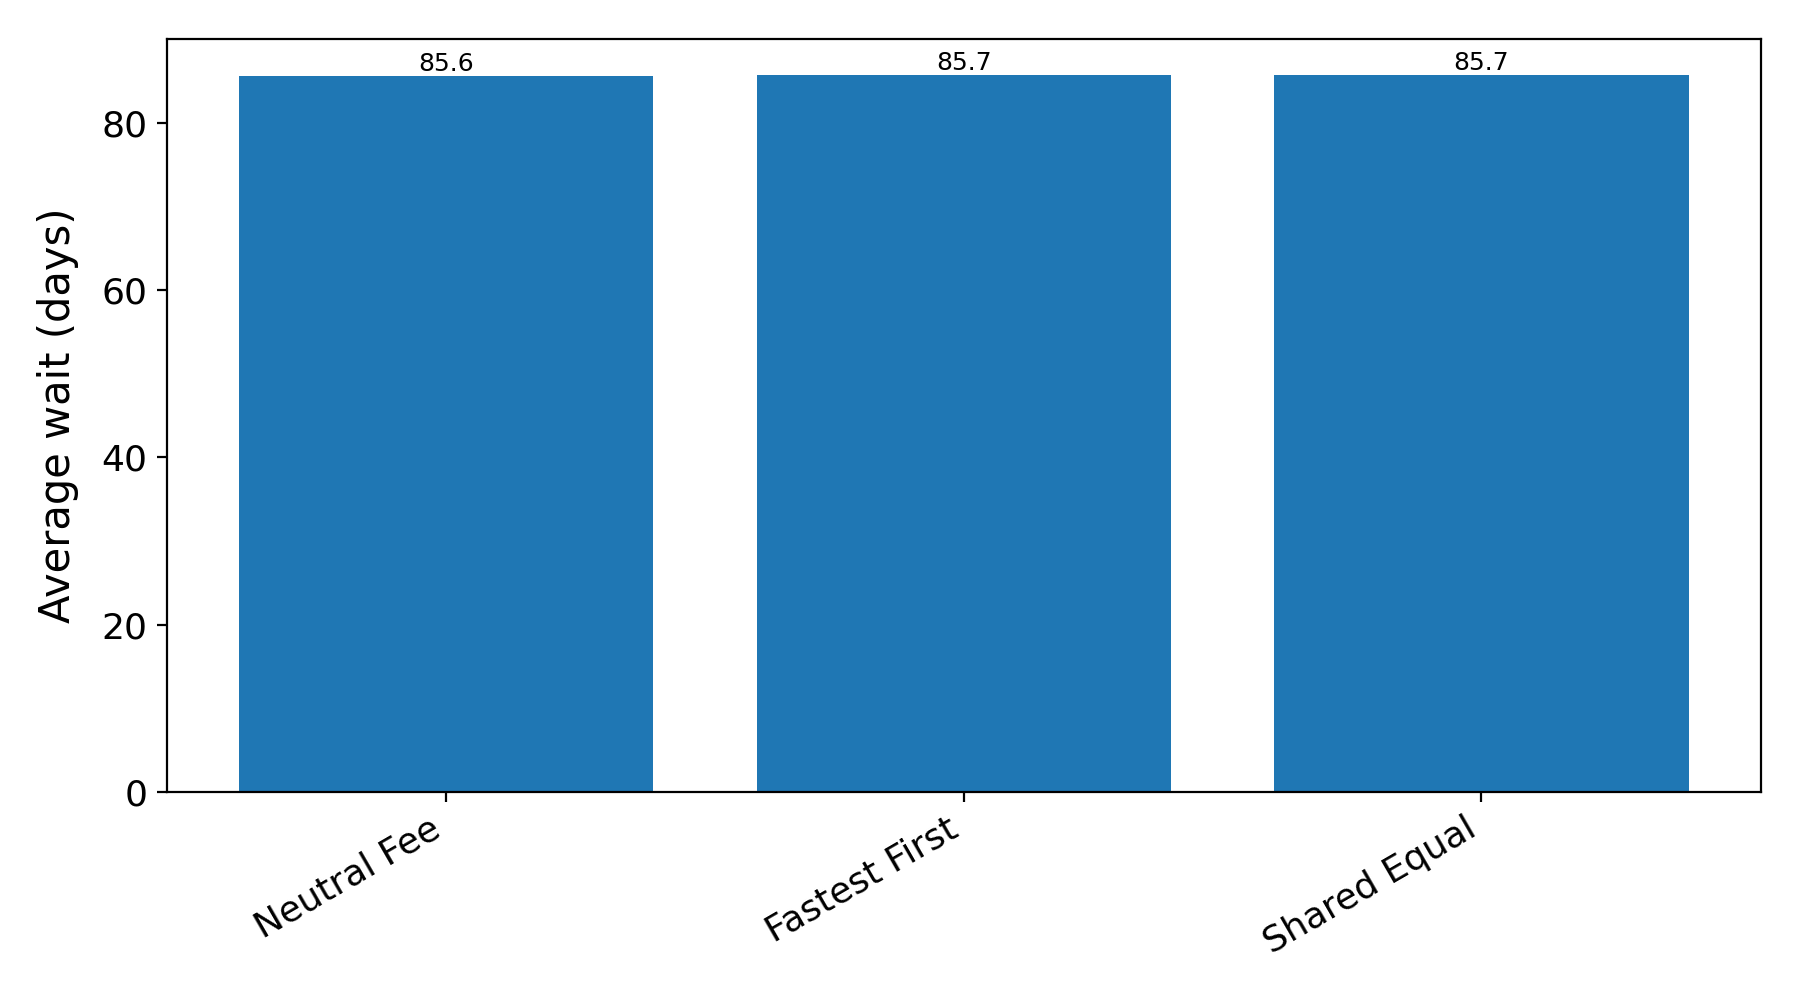
\includegraphics[width=\linewidth]{fig-excluded/fig1_avg_wait_by_policy_nappear.png}
    \caption{Average wait by policy.}
    \label{fig:app-avg-wait}
  \end{subfigure}
  \hfill
  \begin{subfigure}{0.55\linewidth}
    \centering
    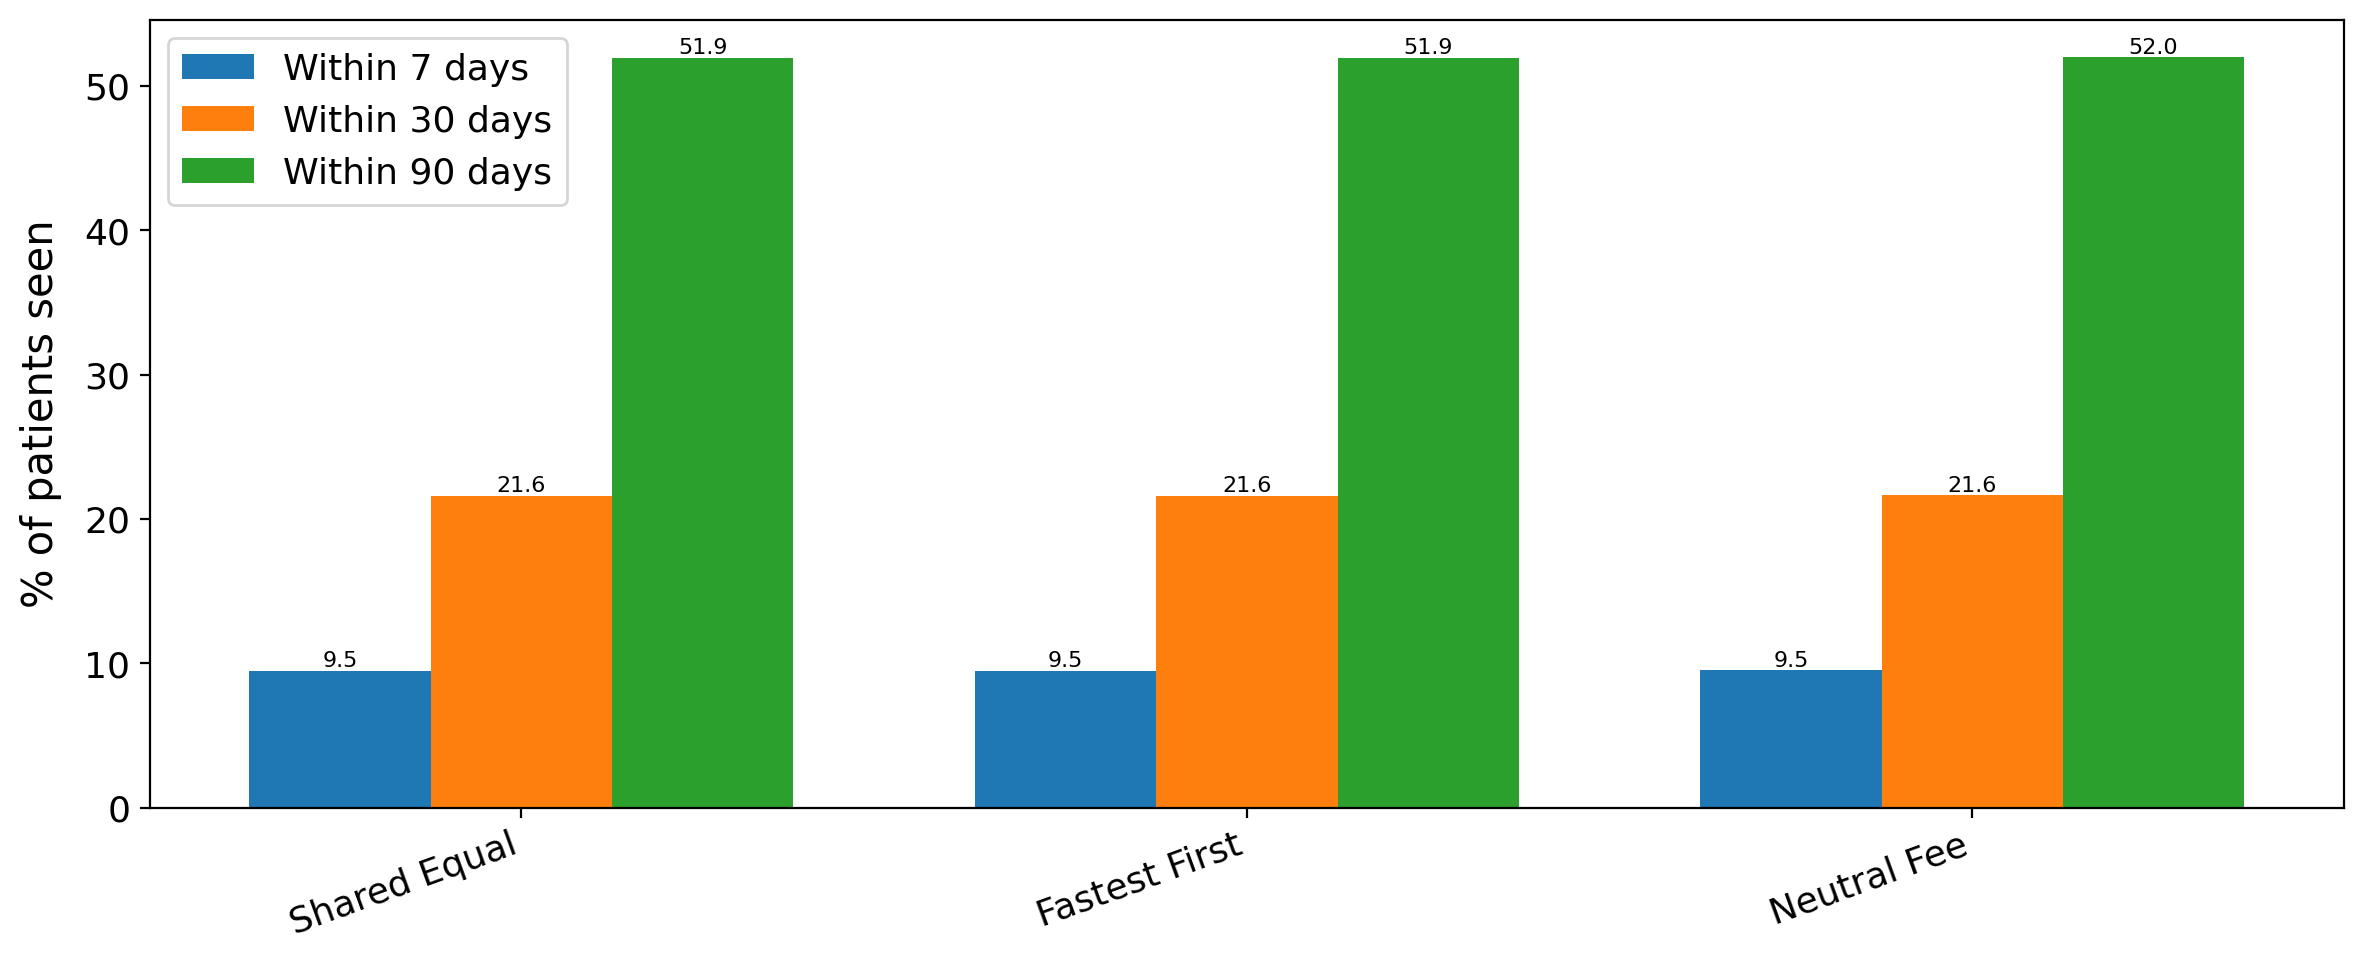
\includegraphics[width=\linewidth]{fig-excluded/fig6a_seen_within_nappear.png}
    \caption{\% seen within 7/30/90 days.}
    \label{fig:app-pct-see}
  \end{subfigure}
  \caption{System KPIs for policies shown only in the appendix.}
  \label{fig:app-sys-kpi-panels}
\end{figure}

\begin{figure}[htbp]
  \centering
  \begin{subfigure}{0.49\linewidth}
    \centering
    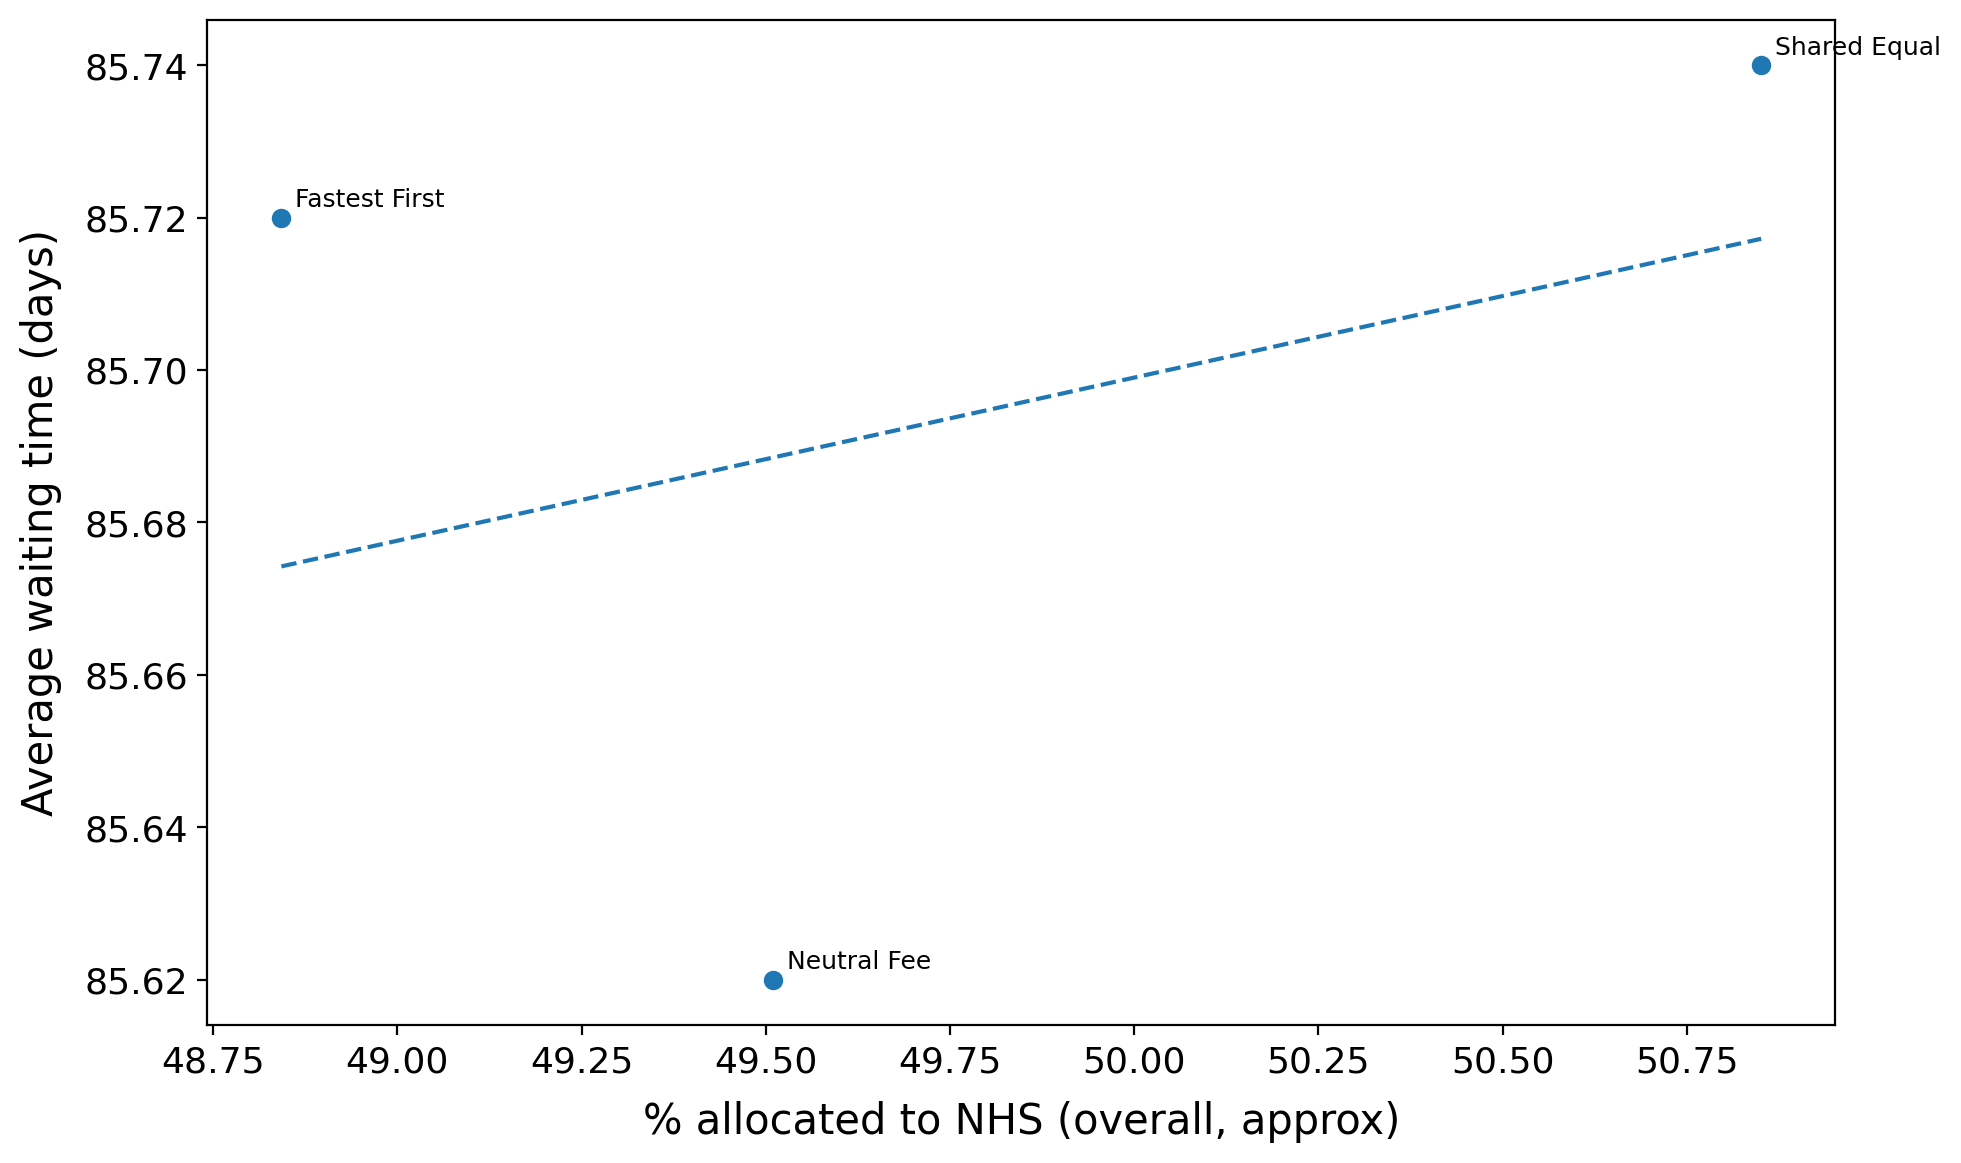
\includegraphics[width=\linewidth]{fig-excluded/fig_wait_vs_nhs_share_nappear.png}
    \caption{Waiting time vs NHS share.}
    \label{fig:app-wait-time-share}
  \end{subfigure}
  \hfill
  \begin{subfigure}{0.49\linewidth}
    \centering
    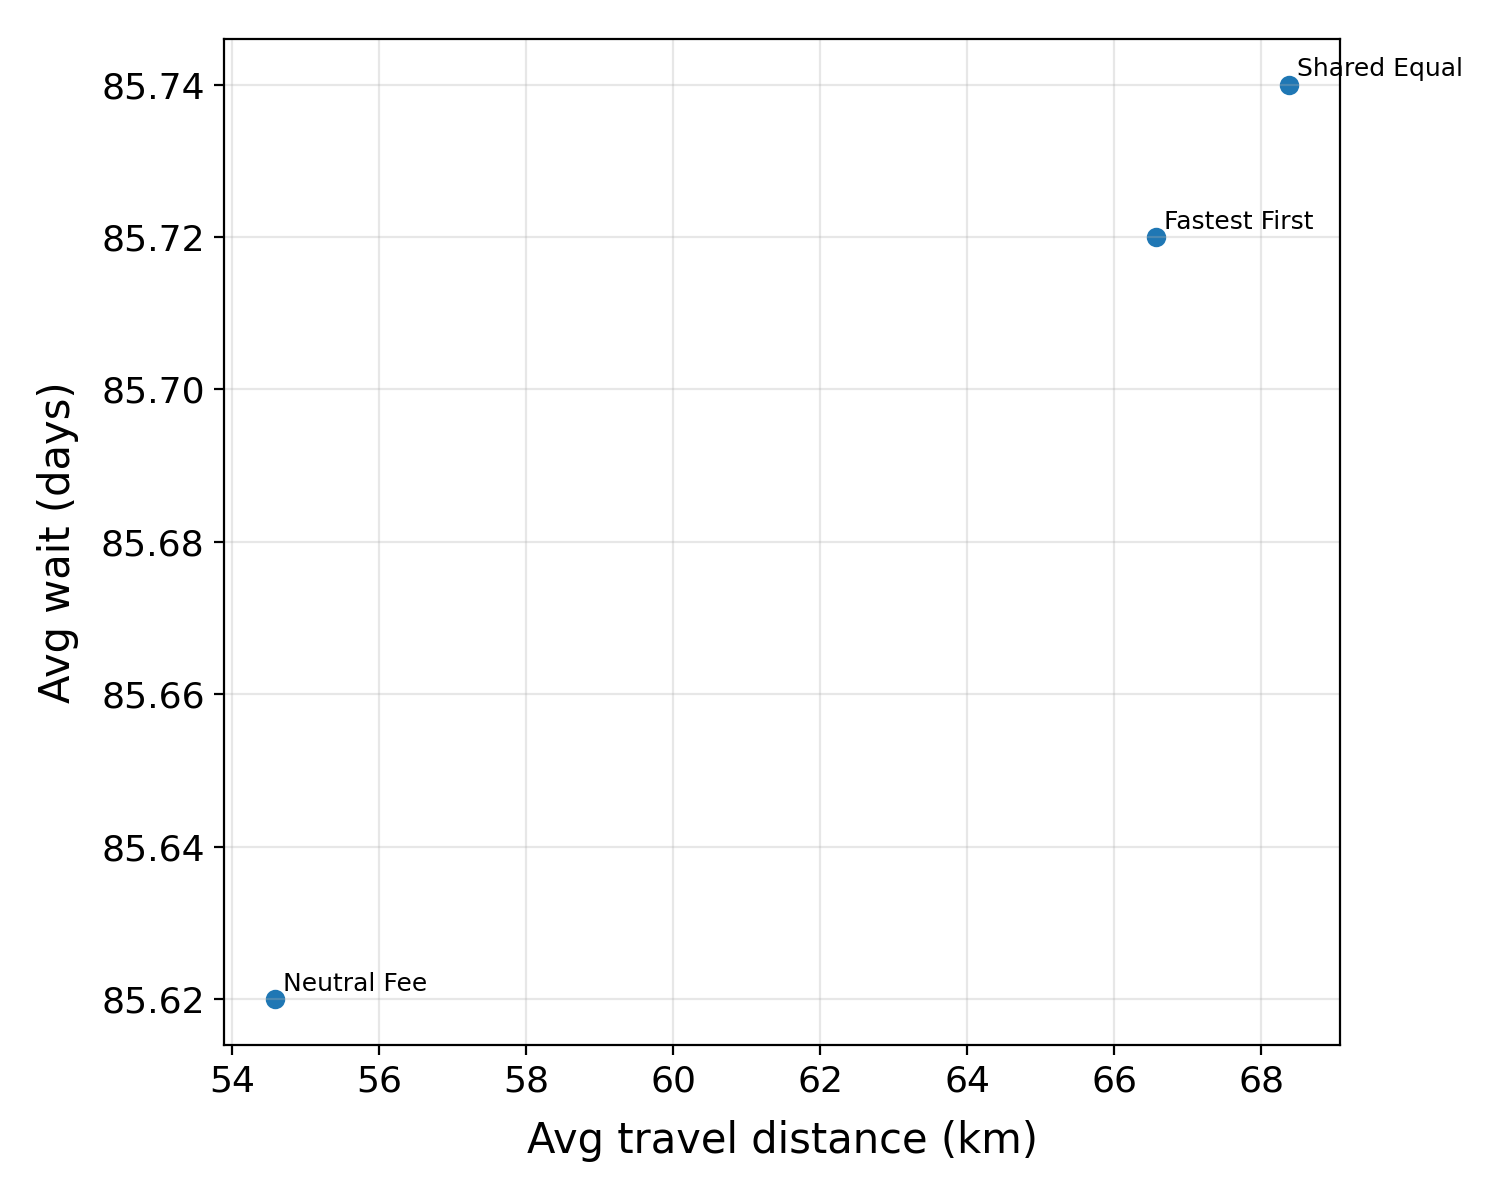
\includegraphics[width=\linewidth]{fig-excluded/fig3_tradeoff_wait_vs_distance_nappear.png}
    \caption{Wait vs travel distance.}
    \label{fig:app-tradeoff-wait}
  \end{subfigure}
  \caption{Trade-offs (appendix set).}
  \label{fig:app-tradeoff-panels}
\end{figure}

\FloatBarrier

\begin{figure}[htbp]
  \centering
  \begin{subfigure}{0.46\linewidth}
    \centering
    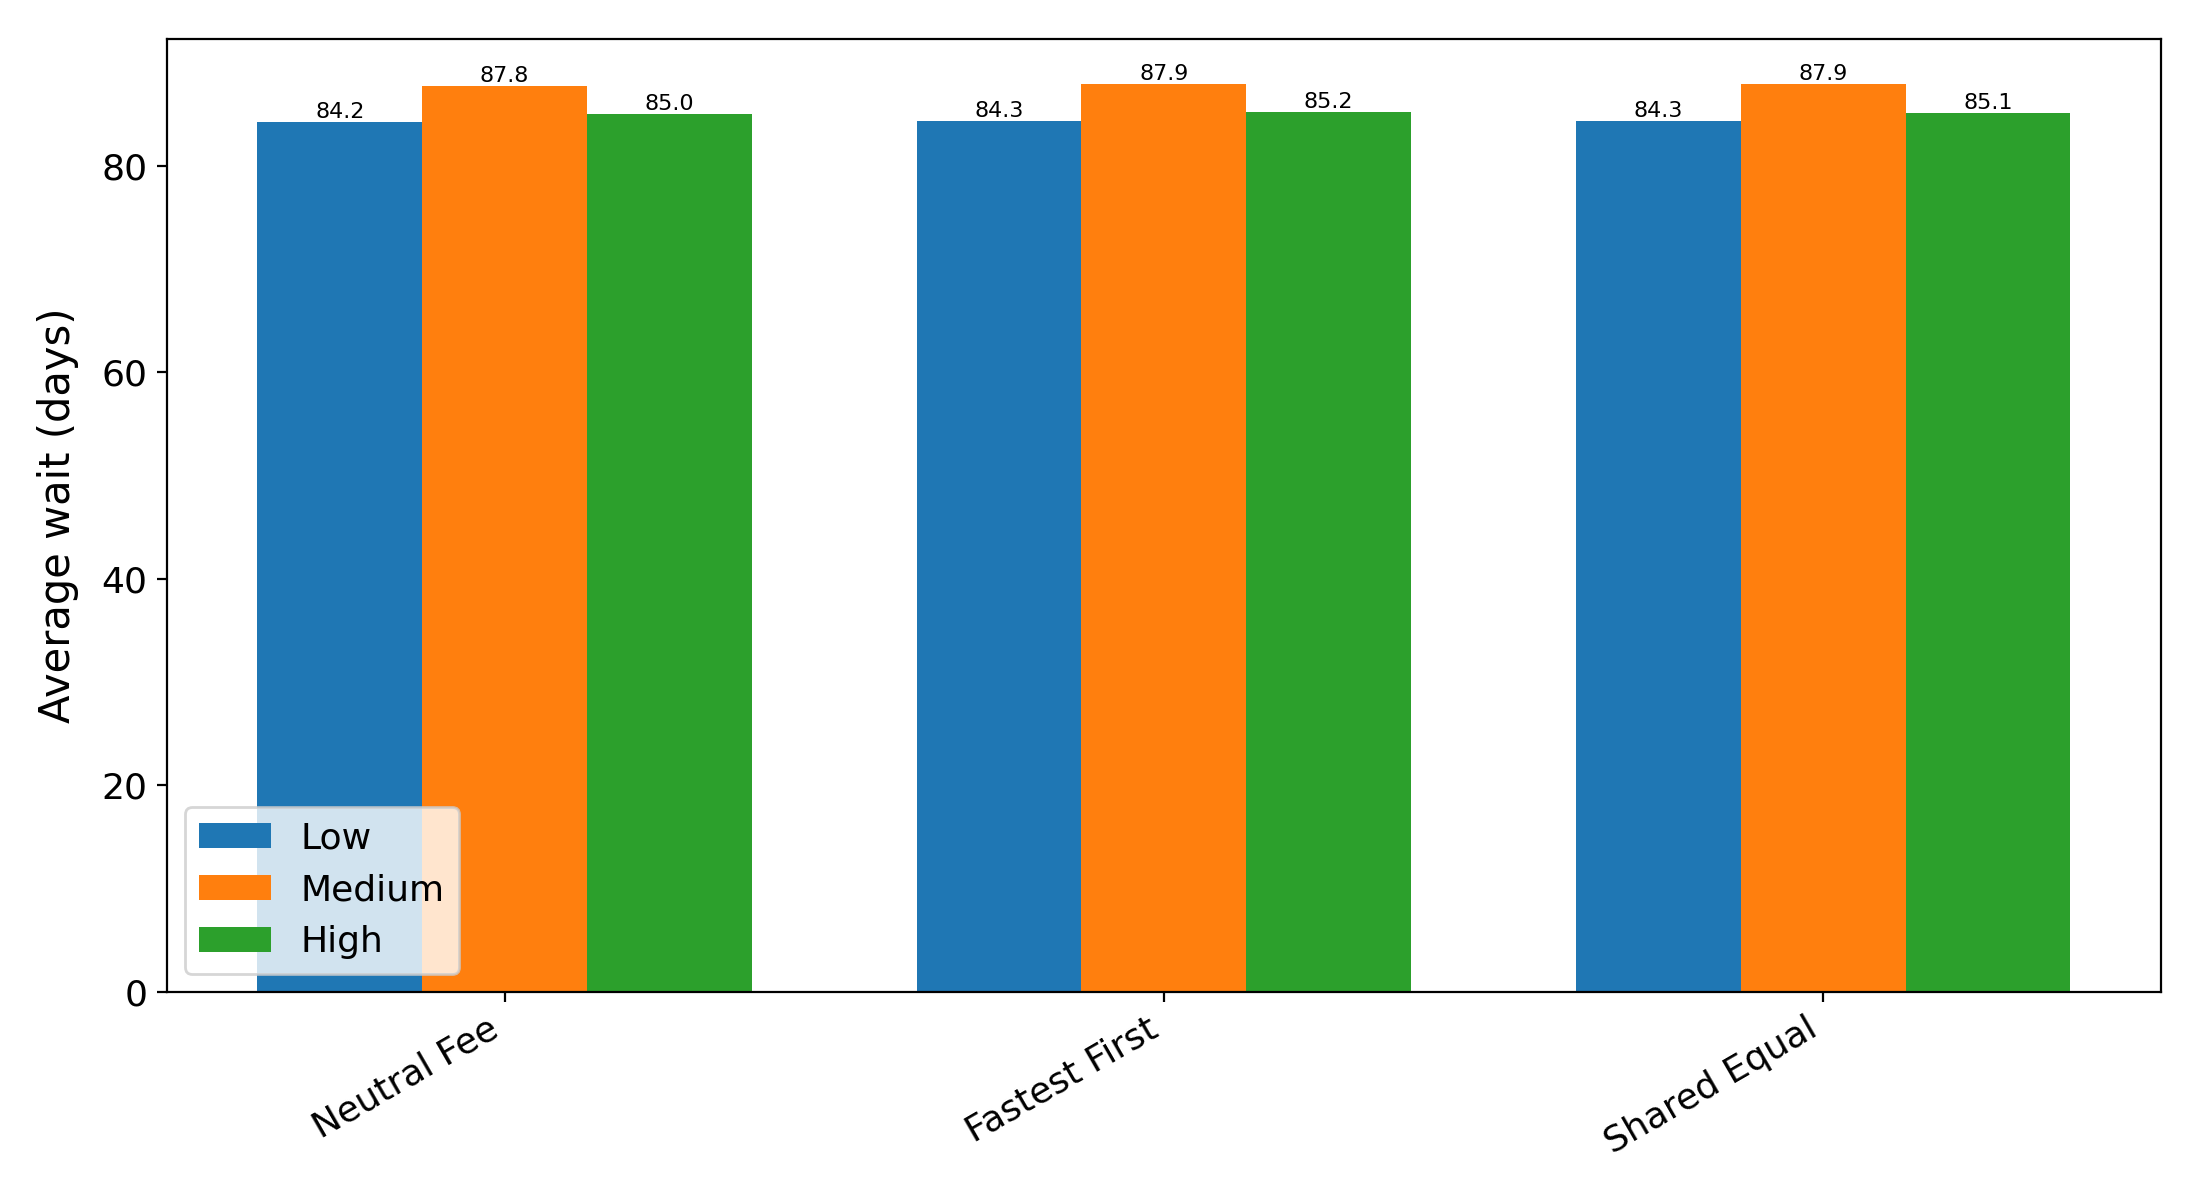
\includegraphics[width=\linewidth]{fig-excluded/fig4_wait_by_complexity_nappear.png}
    \caption{Average wait by complexity and policy.}
    \label{fig:app-avg-wait-by-comp}
  \end{subfigure}
  \hfill
  \begin{subfigure}{0.52\linewidth}
    \centering
    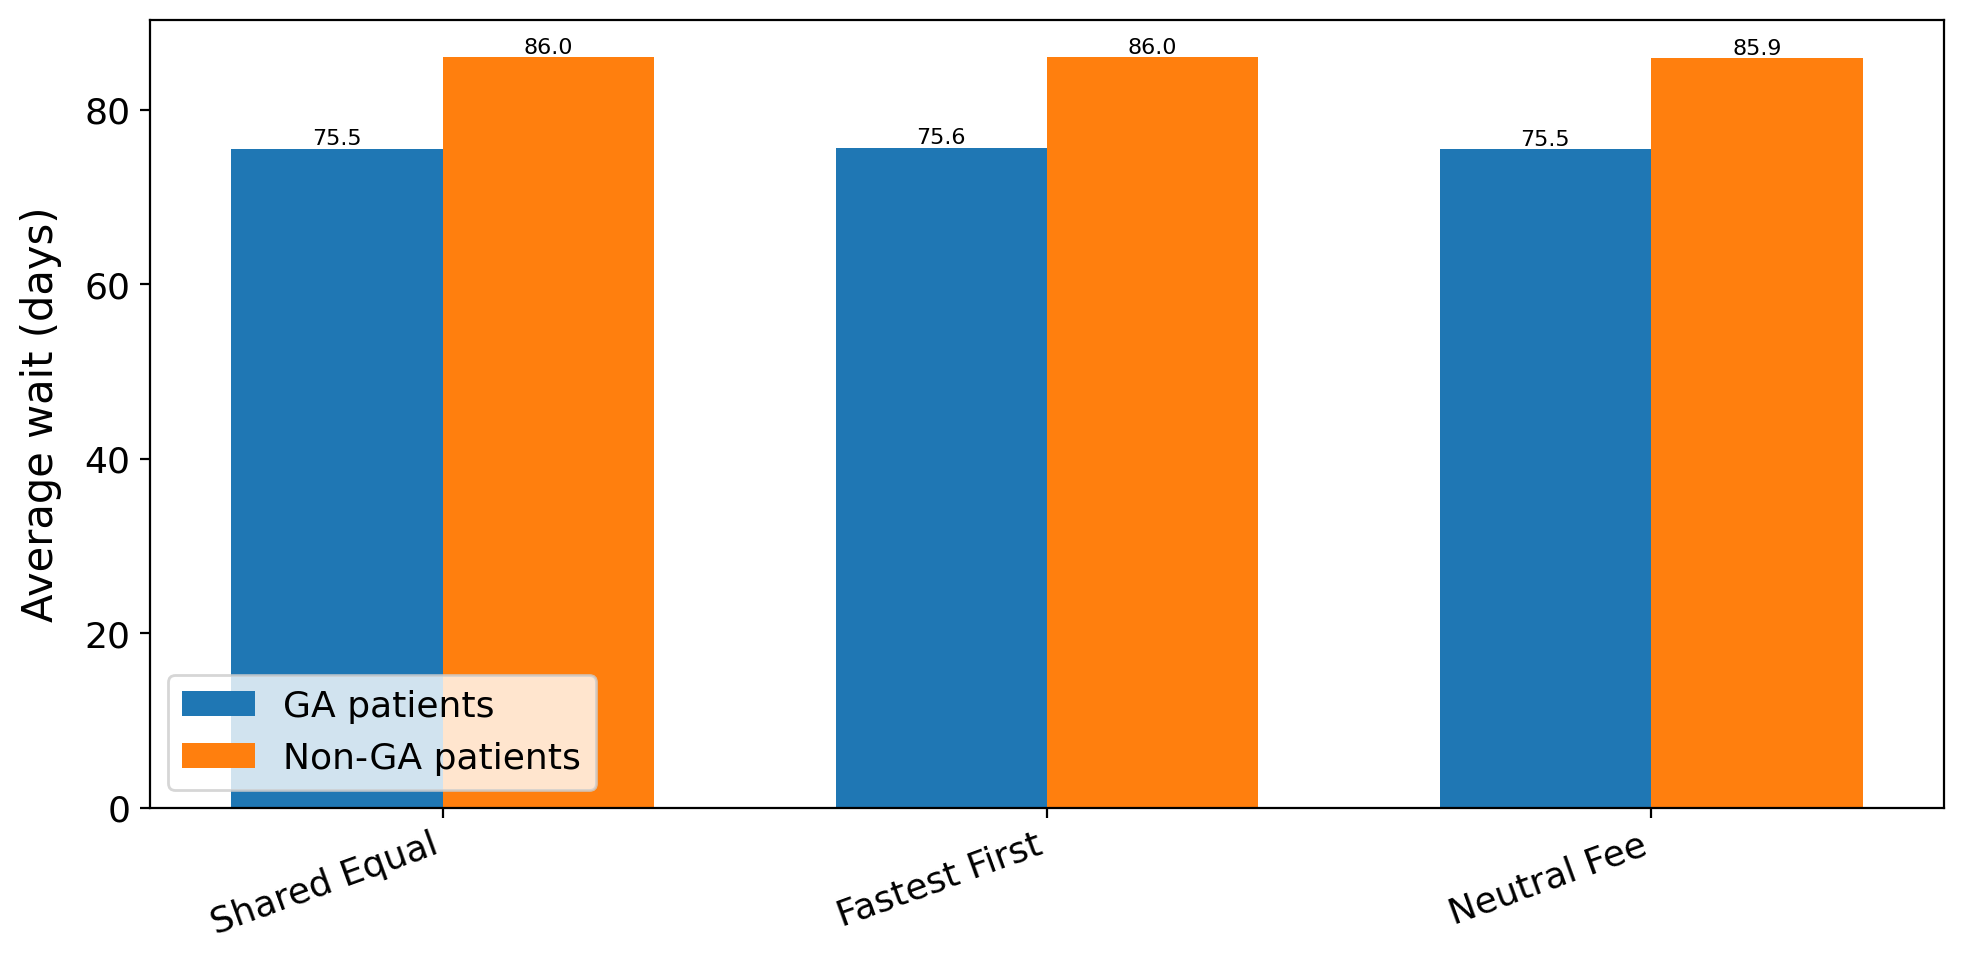
\includegraphics[width=\linewidth]{fig-excluded/fig6b_wait_ga_vs_non_ga_nappear.png}
    \caption{Average wait: GA vs non-GA by policy.}
    \label{fig:app-ga-non-ga}
  \end{subfigure}
  \caption{Patient-level waits.}
  \label{fig:app-patient-waits-panels}
\end{figure}

\begin{figure}[htbp]
  \centering
  \begin{subfigure}{0.49\linewidth}
    \centering
    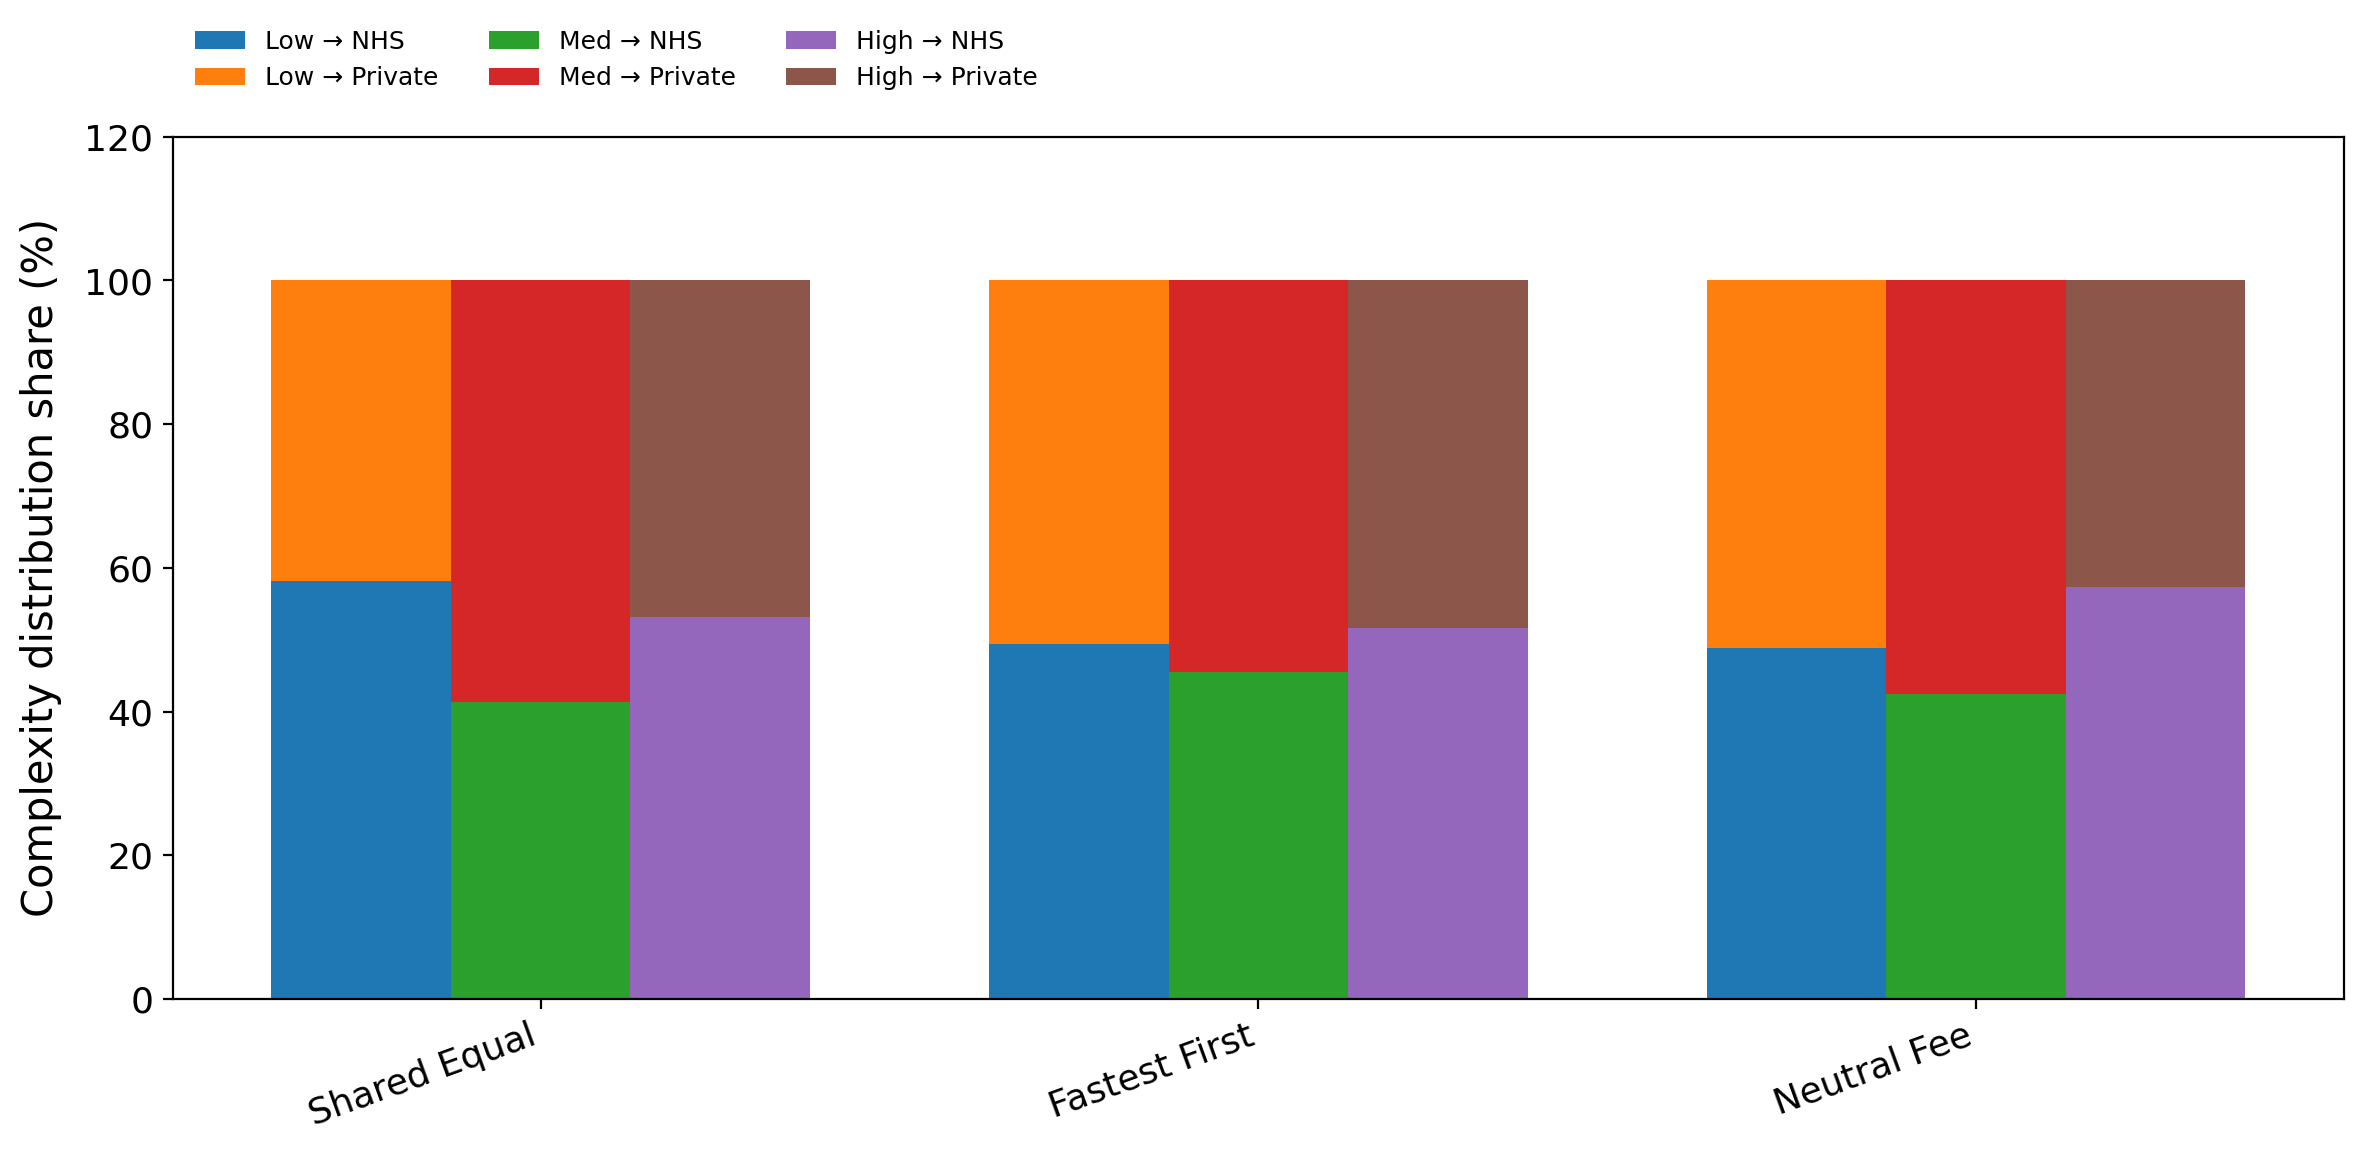
\includegraphics[width=\linewidth]{fig-excluded/fig5a_complexity_mix_by_group_nappear.png}
    \caption{Complexity mix by policy (NHS vs Independent).}
    \label{fig:app-comp-mix}
  \end{subfigure}
  \hfill
  \begin{subfigure}{0.49\linewidth}
    \centering
    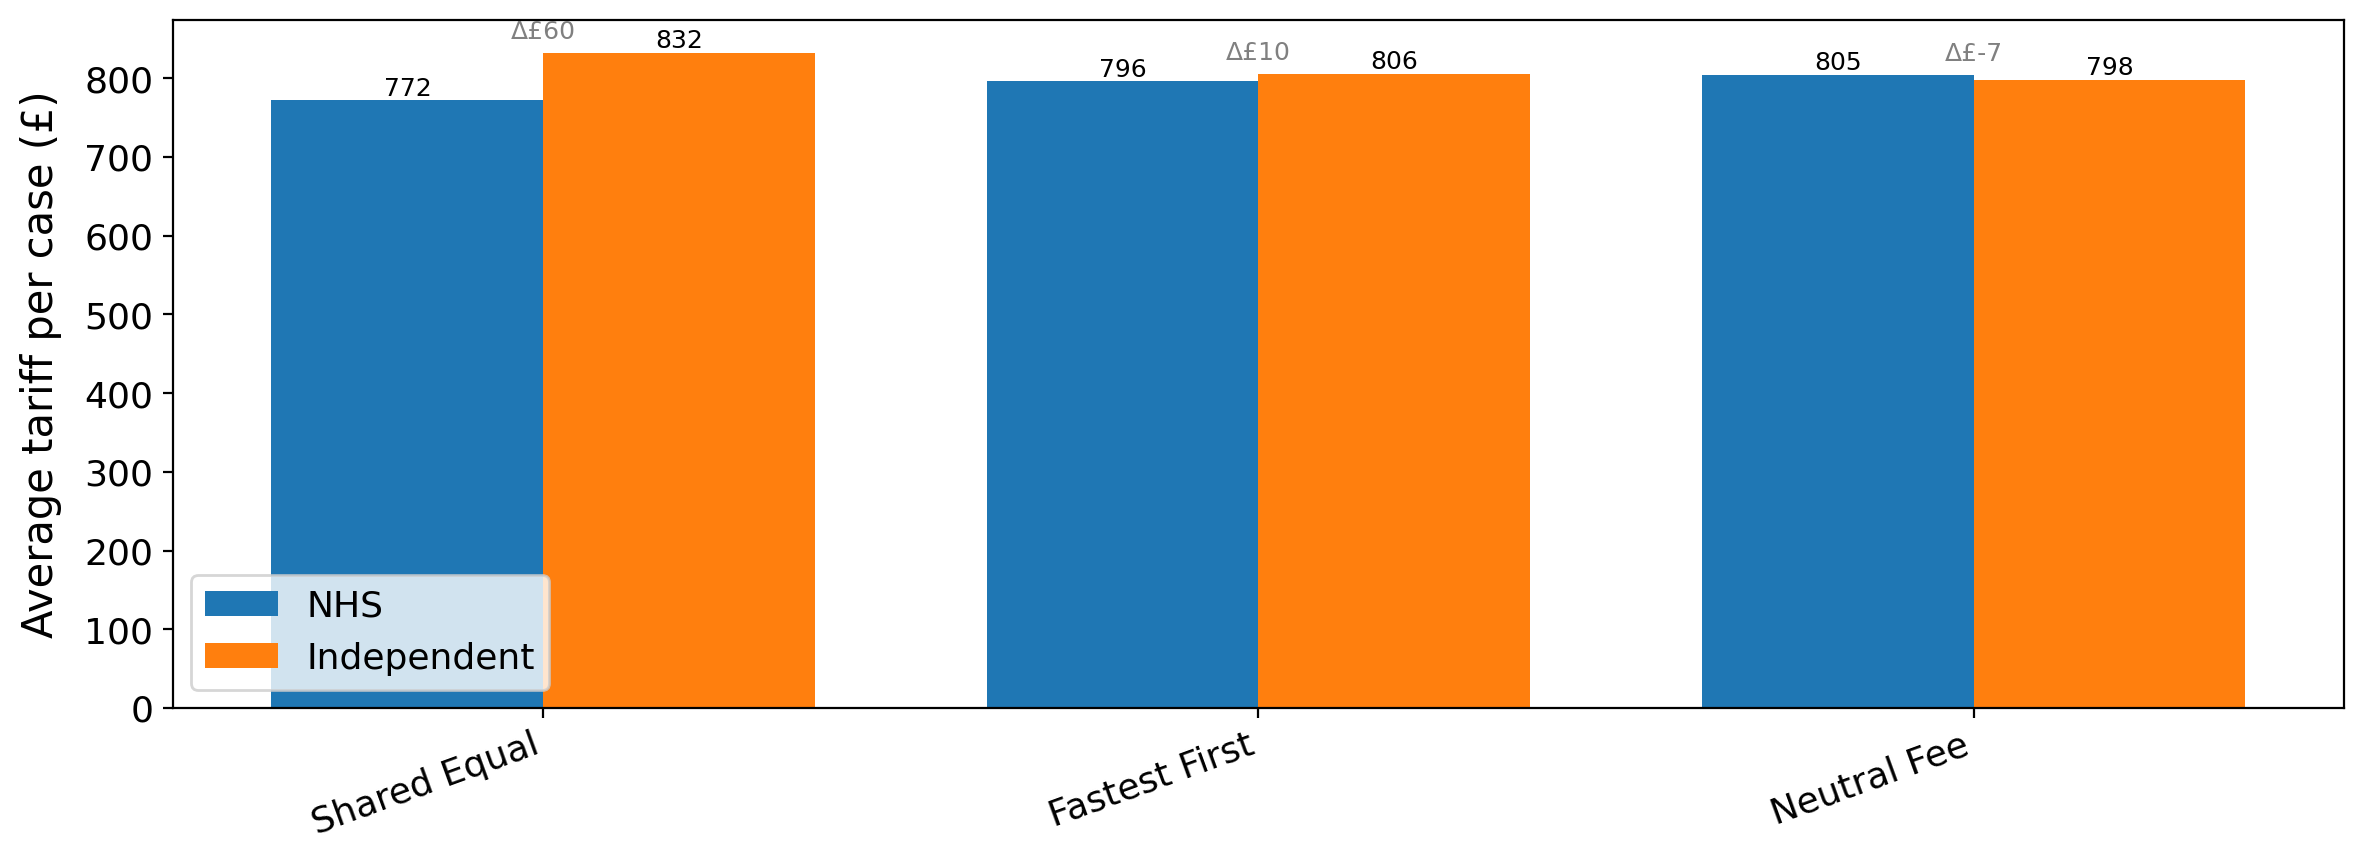
\includegraphics[width=\linewidth]{fig-excluded/fig5b_avg_tariff_by_sector_nappear.png}
    \caption{Average Independent tariff by policy.}
    \label{fig:app-avg-tariff}
  \end{subfigure}
  \caption{Case-mix and incentives (appendix set).}
  \label{fig:app-mix-tariff-panels}
\end{figure}

\FloatBarrier

\begin{table}[htbp]
\centering
\small
\setlength{\tabcolsep}{4pt}
\begin{adjustbox}{width=\linewidth}
\begin{tabular}{lcccccccc}
\toprule
\textbf{Policy} &
\textbf{Mean wait (d)} &
\textbf{Seen$\le$7d (\%)} &
\textbf{Seen$\le$30d (\%)} &
\textbf{Seen$\le$90d (\%)} &
\textbf{Mean dist.\ (km)} &
\textbf{Avg util.\ (\%)} &
\textbf{Unassigned (n)} &
\textbf{Avg tariff (\pounds)} \\
\midrule
Shared Equal   & 85.74 & 9.50 & 21.61 & 51.92 & 68.38 & 59.99 & 0 & 801.29 \\
Neutral Fee    & 85.62 & 9.53 & 21.65 & 51.98 & 54.58 & 60.52 & 0 & 801.29 \\
Fastest First  & 85.72 & 9.50 & 21.61 & 51.92 & 66.57 & 61.98 & 0 & 801.29 \\
\bottomrule
\end{tabular}
\end{adjustbox}
\caption{KPI summaries for policies reported only in the appendix (single-run means).}
\label{tab:app-kpi-single}
\end{table}

\begin{table}[้้h!]
\centering
\small
\setlength{\tabcolsep}{4pt}
\begin{adjustbox}{width=\linewidth}
\begin{tabular}{lccccc}
\toprule
\textbf{Policy} & \textbf{Mean wait (d)} & \textbf{Seen$\le$7d (\%)} &
\textbf{Seen$\le$30d (\%)} & \textbf{Seen$\le$90d (\%)} & \textbf{Mean dist.\ (km)} \\
\midrule
Shared Equal  & 85.75 $\pm$ 0.02 & 9.49 $\pm$ 0.01 & 21.60 $\pm$ 0.01 & 51.91 $\pm$ 0.01 & 68.27 $\pm$ 0.10 \\
Neutral Fee   & 85.75 $\pm$ 0.03 & 9.49 $\pm$ 0.01 & 21.60 $\pm$ 0.01 & 51.91 $\pm$ 0.02 & 54.56 $\pm$ 0.08 \\
Fastest First & 85.71 $\pm$ 0.03 & 9.50 $\pm$ 0.01 & 21.62 $\pm$ 0.01 & 51.92 $\pm$ 0.02 & 66.64 $\pm$ 0.05 \\
\bottomrule
\end{tabular}
\end{adjustbox}
\caption{KPI summaries for policies reported only in the appendix (mean $\pm$ 95\% CI; $r=10$).}
\label{tab:app-kpi-ci}
\end{table}

\section{System-wide KPIs by policy (single-run means)}
\begin{table}[h!]
\centering
\footnotesize
\setlength{\tabcolsep}{4pt}
\begin{adjustbox}{width=\linewidth}
\begin{tabular}{lccccc}
\toprule
\textbf{Policy} & \textbf{Mean wait (d)} & \textbf{Seen$\le$7d (\%)} &
\textbf{Seen$\le$30d (\%)} & \textbf{Seen$\le$90d (\%)} & \textbf{Mean dist.\ (km)} \\
\midrule
Baseline & 112.10 & 7.65 & 10.54 & 33.71 & 58.40 \\
Complexity Balanced & 85.62 & 9.59 & 21.85 & 52.05 & 59.32 \\
Fee Biased & 96.81 & 19.20 & 34.07 & 62.34 & 55.51 \\
ML Balanced (wait+dist+util) & 85.71 & 9.53 & 21.63 & 51.93 & 57.61 \\
\bottomrule
\end{tabular}
\end{adjustbox}
\caption{System-wide KPIs by main policies (single-run means; shown here for cross-reference).}
\label{tab:app-sys-kpi-main}
\end{table}

\clearpage
\section{Additional Sensitivity Analyses}
\begin{figure}[htbp]
    \centering
    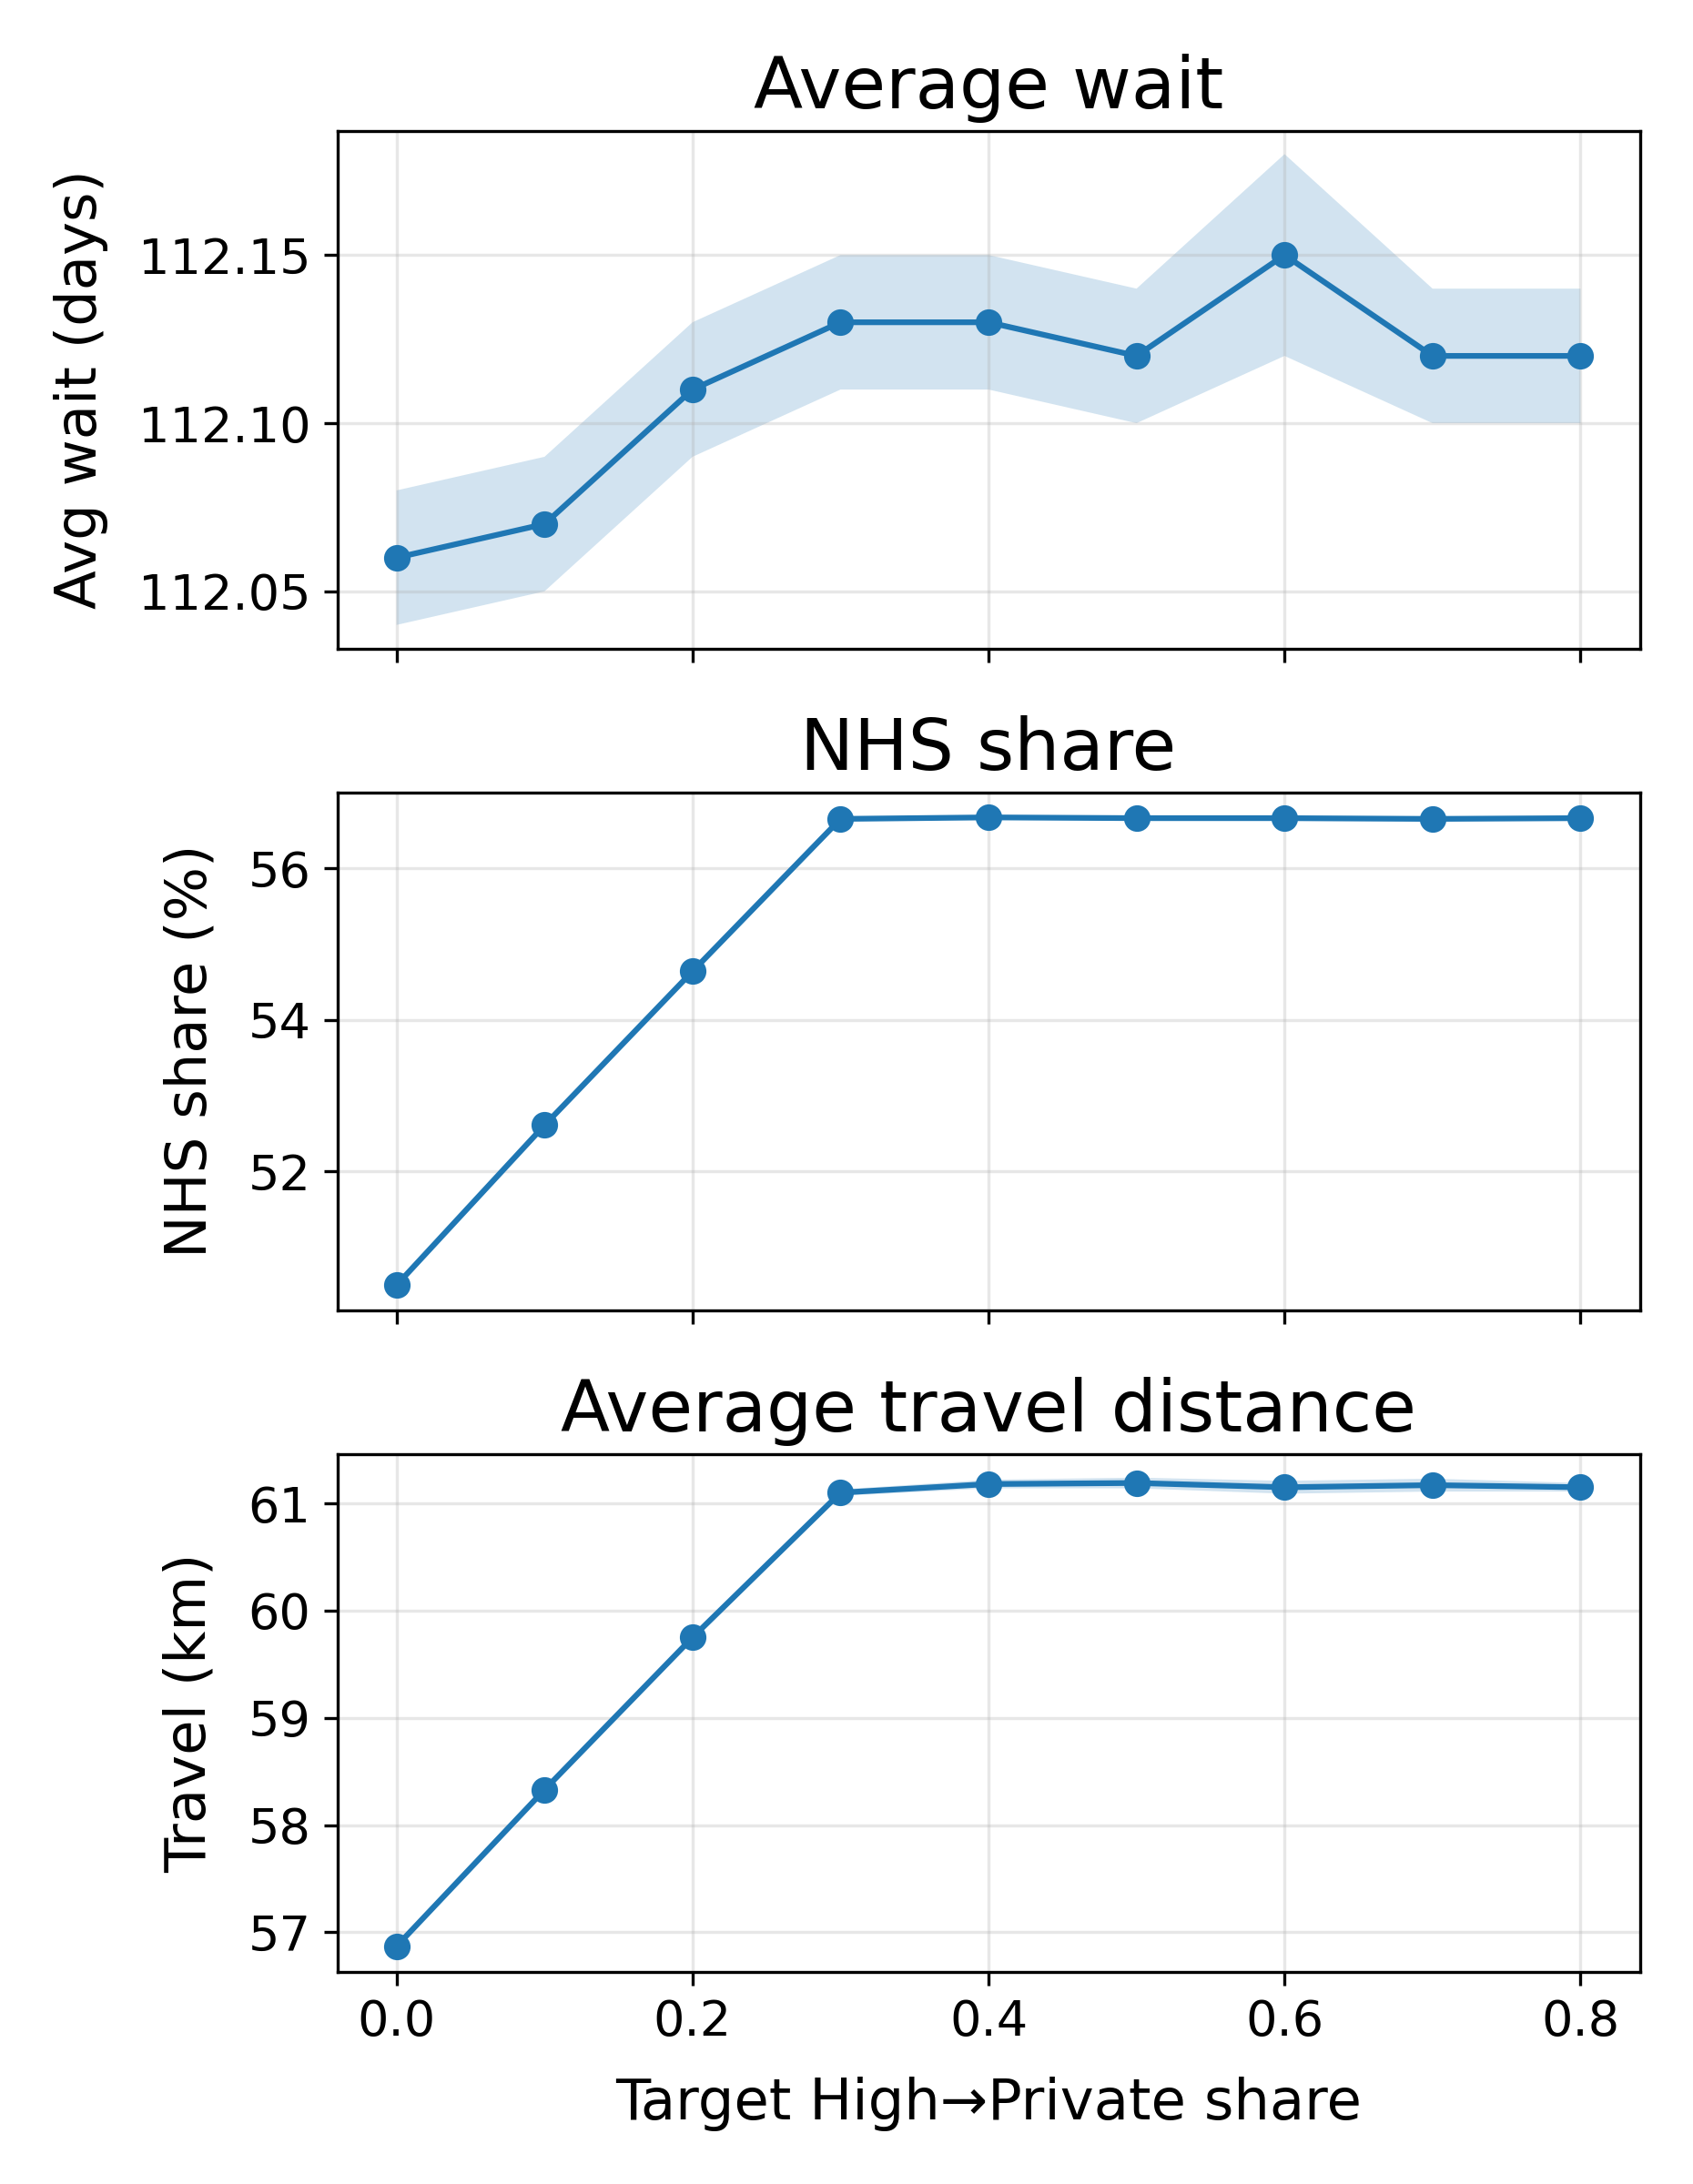
\includegraphics[width=0.7\textwidth]{fig/frontier_combined.png}
    \caption{Sensitivity analysis of targeting a larger share of High-complexity cases to Independent providers (0–80\%). 
    Average waiting time remains flat at $\sim$112 days, NHS share stabilises around 56–57\%, and travel distance rises modestly. 
    These results confirm that under current capacity and GA$\rightarrow$NHS rules, redistributing High cases alone does not materially change system-level outcomes.}
    \label{fig:high-to-private-sensitivity}
\end{figure}
% =============================================================================

\end{document}
